\documentclass[draft=false
              ,paper=a4
              ,twoside=false
              ,fontsize=11pt
              ,headsepline
              ,BCOR10mm
              ,DIV11
              ]{scrbook}
\usepackage[ngerman,english]{babel}
%% see http://www.tex.ac.uk/cgi-bin/texfaq2html?label=uselmfonts
\usepackage[T1]{fontenc}
\usepackage[utf8]{inputenc}
%\usepackage[latin1]{inputenc}
\usepackage{libertine}
\usepackage{pifont}
\usepackage{microtype}
\usepackage{textcomp}
\usepackage[german,refpage]{nomencl}
\usepackage{setspace}
\usepackage{makeidx}
\usepackage{listings}
\usepackage{natbib}
\usepackage[ngerman,colorlinks=true]{hyperref}
\usepackage{soul}
\usepackage{hawstyle}
\usepackage{lipsum} %% for sample text
% Better table
\usepackage{tabularx}

% Better itemize
\usepackage{enumitem}

% For minipages with figures %%
\usepackage{caption}          %
\usepackage{subcaption}       %
%%%%%%%%%%%%%%%%%%%%%%%%%%%%%%%

% Show subsubsection in TOC %
%\setcounter{tocdepth}{3}    %
%\setcounter{secnumdepth}{3} %
%%%%%%%%%%%%%%%%%%%%%%%%%%%%%

%% define some colors
\colorlet{BackgroundColor}{gray!20}
\colorlet{KeywordColor}{blue}
\colorlet{CommentColor}{black!60}
%% for tables
\colorlet{HeadColor}{gray!60}
\colorlet{Color1}{blue!10}
\colorlet{Color2}{white}

%% configure colors
\HAWifprinter{
  \colorlet{BackgroundColor}{gray!20}
  \colorlet{KeywordColor}{black}
  \colorlet{CommentColor}{gray}
  % for tables
  \colorlet{HeadColor}{gray!60}
  \colorlet{Color1}{gray!40}
  \colorlet{Color2}{white}
}{}
\lstset{%
  numbers=left,
  numberstyle=\tiny,
  stepnumber=1,
  numbersep=5pt,
  basicstyle=\ttfamily\small,
  keywordstyle=\color{KeywordColor}\bfseries,
  identifierstyle=\color{black},
  commentstyle=\color{CommentColor},
  backgroundcolor=\color{BackgroundColor},
  captionpos=b,
  fontadjust=true
}
\lstset{escapeinside={(*@}{@*)}, % used to enter latex code inside listings
        morekeywords={uint32_t, int32_t}
}
\ifpdfoutput{
  \hypersetup{bookmarksopen=false,bookmarksnumbered,linktocpage}
}{}

%% more fancy C++
\DeclareRobustCommand{\cxx}{C\raisebox{0.25ex}{{\scriptsize +\kern-0.25ex +}}}

%% TODOS markieren
\newcommand{\TODO}[1]{\colorbox{yellow}{\textcolor{red}{[TODO: #1]}}}

\clubpenalty=10000
\widowpenalty=10000
\displaywidowpenalty=10000

% unknown hyphenations
\hyphenation{
}

%% recalculate text area
\typearea[current]{last}

\makeindex
\makenomenclature

\begin{document}
\selectlanguage{ngerman}

%%%%%
%% customize (see readme.pdf for supported values)
\HAWThesisProperties{Author={Benjamin Burchard}
                    ,Title={Evaluation und Analyse von Visualisierungstechniken für Kommunikationsdaten im Fahrzeug}
                    ,EnglishTitle={Evaluation and analysis of visualisation techniques for communicationdata in a vehicle}
                    ,ThesisType={Master Arbeit}
                    ,ExaminationType={Master Ausarbeitung}
                    ,DegreeProgramme={Master of Science Informatik}
                    ,ThesisExperts={Prof. Dr. Franz Korf \and Prof. Dr. Philipp Jenke}
                    ,ReleaseDate={19. September 2017}
                  }

%% title
\frontmatter

%% output title page
\maketitle

\onehalfspacing

%% add abstract pages
%% note: this is one command on multiple lines
\HAWAbstractPage
%% German abstract
{Schlüsselwort 1, Schlüsselwort 2}%
{Dieses Dokument \ldots}
%% English abstract
{keyword 1, keyword 2}%
{This document \ldots}

\newpage
\singlespacing

\tableofcontents
\newpage
%% enable if these lists should be shown on their own page
%%\listoftables
\listoffigures
%\lstlistoflistings

%% main
\mainmatter
\onehalfspacing

\chapter{Einleitung} % (fold)
\label{cha:einleitung}
% Abschnitt Ethernet Fahrzeugnetz
In zukünftigen automobilen Netzwerken wird vermehrt Ethernet zum Einsatz kommen. Nicht nur die zunehmende Bandbreitenanforderung, durch mehr bandbreitenintensive Geräte im Fahrzeug (Kameras, Laserscanner etc.), verlangt nach einem neuen Übertragungsmedium. Auch die bestehende Diversität der verbauten Bustechnologien und die damit einhergehende Vielschichtigkeit des Fahrzeugnetzes, spricht für eine einheitliche und weniger komplexe Lösung wie sie mit Echtzeit Ethernet gegeben wäre. Diese Umstrukturierung bringt neue Metriken für die Daten des Fahrzeugnetzes mit sich. Um diese für das automobile Echtzeit-Ethernet zu analysieren, benötigt man eine hinreichende visuelle Aufbereitung dieser Kommunikationsdaten und deren Eigenschaften, wie Jitter oder Latenz. Kommunikationsdaten sind im Grunde alle Daten welche über das Netzwerk transportiert, also kommuniziert werden. Um Kommunikationsdaten, sowie die Eigenschaften dieser, zu visualisieren gibt es viele verschiedene Möglichkeiten und Techniken. Informationsvisualisierung versucht mit Hilfe von geeigneten grafischen Repräsentationen Nutzerinformationen zu optimieren. Diese bildlichen Darstellungsformen sollen bei der Interpretation und Auswertung von großen Datenmengen helfen. In vorhandenen Automobilen Ethernet Fahrzeugnetzen entstehen bis zu 3 Gigabyte Daten pro Stunde \cite{core_2017}. Viele moderne Fahrzeuge kommunizieren bereits mit mehr als 100 ECUs (Electronic Control Units) innerhalb ihrer Netze \cite{broy_cross-layer_2011}. Anhand dieser Zahlen lässt sich sagen, dass einen Bedarf sowie Nutzen für Visualisierungen und Werkzeuge besteht, welche die Daten abstrahieren und dem Nutzer verständlich machen.

% Abschnitt visualisierung
Die Visualisierung von Daten zielt darauf ab, Daten durch eine grafische Interpretation verwertbar zu machen. Durch die Aufbereitung von Daten entsteht ein Mehrwert für den Nutzer, im Falle dieser Arbeit für den Anwender der Visualisierung oder des Werkzeugs zur Darstellung von Netzwerkkommunikationsdaten im internen Fahrzeugnetzwerk. Visualisierungen ermöglichen es, auf mehr als nur einem Weg, rohen Daten einen Sinn zu verleihen. Das Abbilden der Datenattribute auf visuelle Eigenschaften wie Position, Form, Farbe und Größe wird eingesetzt um Nutzern die Wahrnehmung und Interpretation von Mustern innerhalb der Daten zu erleichtern \cite{shneiderman_designing_2005}. Damit visuelle Analyse Tools effektiv genutzt werden können, müssen diese eine fließende und flexible Nutzung von Visualisierungen ermöglichen. 
\iffalse %%%%%%%%%%%%%%%%%%%%%%%%%%%%%%%%%%%%%%%%%%%%%%%%%%%%%%%%%%%%%%%%%%%%%%%%%%%%%%%%%%%%%%%%%%%%%%%%%%%%%%%%%%%%%%%%%%%%%%%%%%%%%%%%%%%%%%%%%%%%%%%%%%%%%%%%%%%%%%%%%%%%%%%%
%\TODO{Was machen wir mit Daten? Vielleicht aus der Simulation?}
\fi      %%%%%%%%%%%%%%%%%%%%%%%%%%%%%%%%%%%%%%%%%%%%%%%%%%%%%%%%%%%%%%%%%%%%%%%%%%%%%%%%%%%%%%%%%%%%%%%%%%%%%%%%%%%%%%%%%%%%%%%%%%%%%%%%%%%%%%%%%%%%%%%%%%%%%%%%%%%%%%%%%%%%%%%%
% Abschnitt Evaluationen brauchen wir weil
Um geeignete Visualisierungen und Werkzeuge für das Themenfeld der Netzwerkkommunikation im Fahrzeugethernet zusammenzutragen, müssen vorhandene Visualisierungen hinsichtlich ihrer Verwendbarkeit im genannten Themenfeld eingeschätzt werden. Dieser Teil der Arbeit soll mit Hilfe einer Evaluation verwirklicht werden. Es gibt eine breite Auswahl an Evaluationstechniken, welche alle zum Ziel haben eine Software oder ein Softwareprodukt auf verschiedenste Eignungen hin zu untersuchen. Hier muss eine differenzierte Auswahl erfolgen welche Technik oder Techniken für diesen Themenkomplex, aber für den spezifischen Fall der Evaluation in einer Masterarbeit geeignet sind. Der grobe Aufbau und Fluss dieser Arbeit wird in Abbildung \ref{fig:aufbaugrob} dargestellt. 

\begin{figure}[htbp]
  \centering
  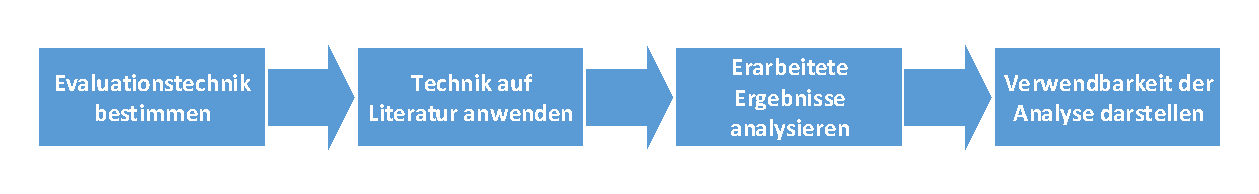
\includegraphics[width=\textwidth]{img/Aufbau_grob.pdf}
  \caption{Grober Aufbau der Arbeit}
  \label{fig:aufbaugrob}
\end{figure}


% Kommentar Korf:
% Aus diesem Bild geht hervor, dass Sie Daten evaluieren, ziehen daraus Schlüsse / leiten Anforderungen ab. Und dann ist Schluss. 
% Das bedeutet auch, dass Sie bei der Evaluation eine signifikante Tiefe erreichen müssen. Das beutet eine detaillierte Literaturarbeit, die sich nicht nur auf die Kommunikation 
% im Auto bezieht. Weiterhin müssen Sie die spezifischen Aspekte der Kommunikation im Auto deutlich herausarbeiten. Sie müssen daraus Schlüsse ziehen und diese untermauern.
% Wollen Sie auf realen Daten evaluieren. Dann sorgen Sie jetzt dafür, dass Sie genug Daten haben. Oftmals muss man subjektive Analysen mit konkreten Daten untermauern.

% META ANALYSE? (oder) DATEN AUS SIMULATION?


% Zielsetzung
Das Ziel dieser Arbeit besteht darin, eine für die Herausforderungen der Analyse eines modernen Fahrzeugnetzwerk geeignete Visualisierungstechnik zu finden. Zum Erreichen dieses Ziels werden Grundlagen der Bereiche Evaluation und Visualisierung erarbeitet. Dies geschieht in Kapitel \ref{cha:einfuhrung_in_das_umfeld}. Die Grundlagen sollen als Einstiegspunkt in die Arbeit fungieren. Es werden Grundlagen aus diesen beiden Themenkomplexen vorgestellt, da beide zum Verständnis der weiteren Kapitel beitragen. Evaluationen für die spätere Wahl einer geeigneten Evaluationstechnik und Visualisierungen für die schlussendliche Bewertung ausgewählter Visualisierungstechniken. Anschließend werden in Kapitel \ref{cha:anforderungsanalyse}, zunächst allgemeine Anforderungen an Visualisierungen und Visualisierungswerkzeuge erarbeitet. Darauf aufbauend werden als Abschluss des Kapitels Automotive spezifische Anforderungen erarbeitet. Diese Anforderungen sind nötig, damit im der späteren Evaluation der Visualisierungstechniken die Anforderungen zur Bewertung angeführt werden können.
In Kapitel \ref{cha:evaluationsbasis} werden Evaluationstechniken in Hinblick auf deren Einsatzfähigkeit im Feld der Visualisierung von Fahrzeugkommunikationsdaten und deren Werkzeuge untersucht. Es gibt eine Vielzahl an Evaluationsmethoden und die richtige Technik zu wählen ist für aussagekräftige Evaluationsergebnisse entscheidend. Die Erarbeitung der einer geeigneten Evaluationstechnik erfolgt durch die Auswertung drei ausgewählter Metaanalysen, welche sich hauptsächlich mit Evaluationsmöglichkeiten im Visualisierungsbereich beschäftigen. Unter Zuhilfenahme der erarbeiteten Evaluationstechniken wird dann im Folgekapitel \ref{cha:evaluation} spezifische Literatur ausgewertet. Damit ist gemeint das hier Literatur speziell aus dem Bereich der Netzwerkvisualisierung ausgewertet wird, mit Hauptaugenmerk auf die Darstellung von Kommunikationsdaten im Fahrzeug. Aus der Analyse der Literatur ergeben sich die Anwendbarkeit der Visualisierungstechniken für den Automotive Bereich. Diese erarbeiteten Techniken können somit eine Grundlage für die Entwicklung neuer Visualisierungssystemen und Werkzeuge bilden. Kapitel \ref{cha:fazit_und_ausblick} enthält die Schlussbetrachtung der Arbeit und gibt einen Ausblick auf mögliche weiterführende Konzepte und Einsatzmöglichkeiten der Ergebnisse der Arbeit gegeben. 
Zusammenfassend ergeben sich mehrere konkrete Teilziele dieser Arbeit. Es werden konkrete Anforderungen für zukünftige und aktuelle Darstellungsformen und die zugehörige Software zusammengestellt. Geeignete Evaluationsmethoden für die Analyse von Visualisierungstechniken im Bereich der Visualisierung von Fahrzeugkommunikation werden erarbeitet. Unter Zuhilfenahme der Evaluatinsmethoden werden potentiell Verwendbare, für den Fahrzeugbereich neue, Visualisierungstechniken zusammengetragen und auf ihre Einsatzmöglichkeiten in der Analyse von Kommunikationsdaten im Fahrzeug hin überprüft.
% chapter einleitung (end)

%%%%%%%%%%%%%%%%%%%%%%%%%%%%%%%%%%%%%%%%%%%%%%%%%%%%%%%%%%%%%%%%%
%%%                         CHAPTER 2                         %%%
%%%%%%%%%%%%%%%%%%%%%%%%%%%%%%%%%%%%%%%%%%%%%%%%%%%%%%%%%%%%%%%%%
\chapter{Einführung in das Umfeld} % (fold)
\label{cha:einfuhrung_in_das_umfeld}
In der \nameref{cha:einleitung} wurde erläutert warum Visualisierungen für die Darstellung der Netzwerkkommunikationsdaten im Fahrzeug wichtig sind. Dieses Kapitel skizziert die Position dieser Arbeit im Bezug auf das wissenschaftliche Umfeld. Der Kernbereich beschäftigt sich mit Visualisierungen aus dem Automotive Bereich. Im speziellen mit Darstellungen für die Kommunikationsdaten und deren Metriken im modernen Automotive Realtime Ethernet. Neben diesem Hauptbereich gibt es mehrere weitere angrenzende Themen, die für die Arbeit von Bedeutung sind. In der folgenden Übersicht \ref{fig:theme_overview} sind diese Bereiche dargestellt. Das Umfeld ist im Wesentlichen in drei Teile gegliedert, Evaluation, Werkzeuge und Visualisierungen sowie Anforderungen und die Analyse dieser. 

\begin{figure}[htbp]
  \centering
  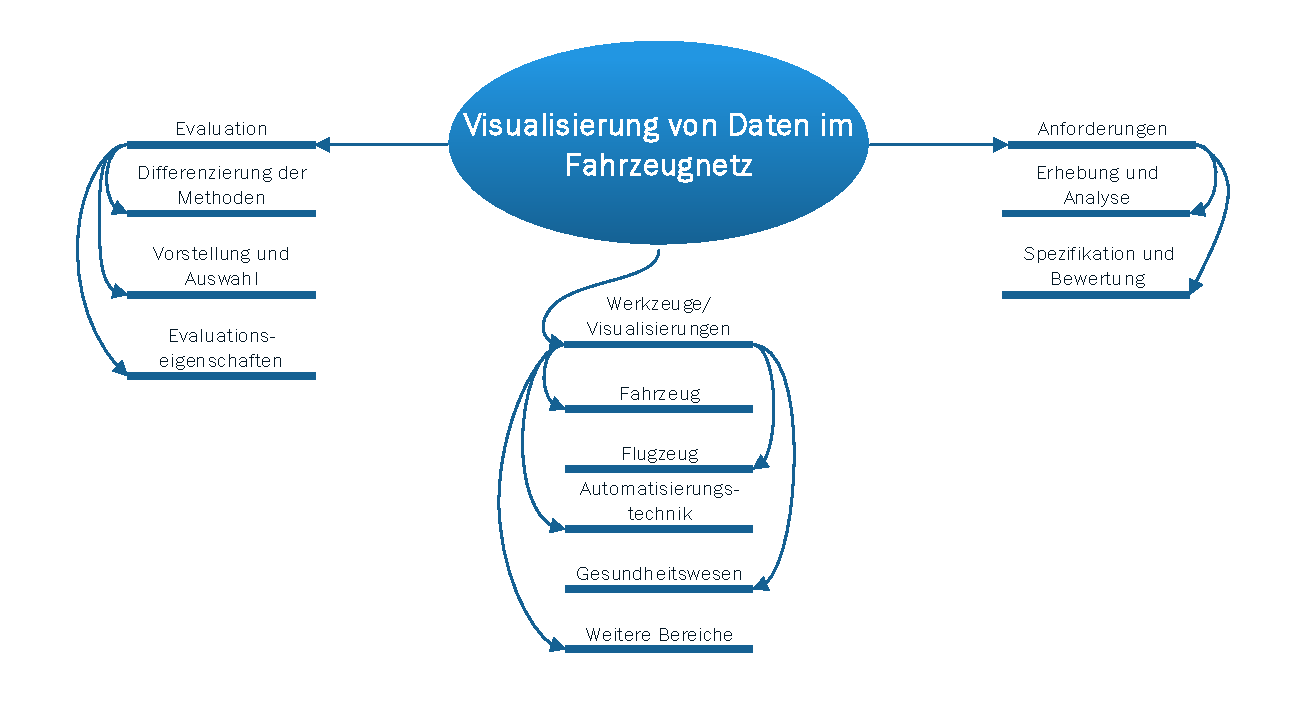
\includegraphics[width=\textwidth]{img/theme_overview.pdf}
  \caption{An diese Arbeit angrenzende wissenschaftliche und wirtschaftliche Bereiche}
  \label{fig:theme_overview}
\end{figure}

Im Abschnitt \ref{sec:grundlagen_der_evaluation} werden die Grundlegenden Evaluationsmethoden vorgestellt. Es wird die Vorarbeit für das Kapitel \nameref{cha:evaluationsbasis} geleistet, welches die geeignetste Technik für die Visualisierung von Netzwerkdaten im Fahrzeugnetz herausarbeitet. Abschnitt \ref{sec:einfuhrung_in_grundlegende_visualisierungen} widmet sich der Betrachtung von Visualisierungen und Werkzeugen, nicht nur aus dem Automotive Bereich, sondern auch aus angrenzenden Bereichen. Der Abschnitt befasst sich weiterhin damit welches diese Bereiche sind und warum diese in Frage kommen. 
% Soll das raus? Es steht aber mit in der Darstellung oben... Vielleicht verweis auf nächstes Kapitel, was ja Anforderungen ist
\iffalse %%%%%%%%%%%%%%%%%%%%%%%%%%%%%%%%%%%%%%%%%%%%%%%%%%%%%%%%%%%%%%%%%%%%%%%%%%%%%%%%%%%%%%%%%%%%%%%%%%%%%%%%%%%%%%%%%%%%%%%%%%%%%%%%%%%%%%%%%%%%%%%%%%%%%%%%%%%%%%%%%%%%%%%%
Der abschließende Teil dieses Kapitels, \nameref{sec:anforderungen_und_analyse}, geht auf die Anforderungen an Visualisierungen ein. Es wird \dots 
\fi      %%%%%%%%%%%%%%%%%%%%%%%%%%%%%%%%%%%%%%%%%%%%%%%%%%%%%%%%%%%%%%%%%%%%%%%%%%%%%%%%%%%%%%%%%%%%%%%%%%%%%%%%%%%%%%%%%%%%%%%%%%%%%%%%%%%%%%%%%%%%%%%%%%%%%%%%%%%%%%%%%%%%%%%%

\section{Grundlagen der Evaluation} % (fold)
\label{sec:grundlagen_der_evaluation}
Im Bereich der Evaluation beschäftigt sich die Arbeit mit der Frage welche Techniken zur Evaluation von Visualisierungen und Interfaces sinnvoll in diesem Themenkomplex einsetzbar sind. Es wird herausgearbeitet welche Evaluationsmöglichkeiten es gibt und welche, aufgrund Ihrer Ergebnisse und Anwendungsgebiete, am geeignetsten erscheinen. Dieser Abschnitt zeigt grundlegende Evaluationsmethoden und deren Anforderungen sowie nutzen. In Kapitel \ref{cha:evaluationsbasis} wird dann eine der vorgestellten Methoden ausgewählt und als Grundlage für die Literaturanalyse verwendet. Die Evaluationstechnik wird zum einen nach ihrer Eignung zur Evaluation von Visualisierungen gewählt und zum anderen nach der Ausführbarkeit im Rahmen einer Masterarbeit.
Bevor die Techniken zur Evaluation vorgestellt werden, folgt zunächst ein Einblick wie zwischen Evaluationen differenziert wird, weshalb Evaluation verwendet wird und was damit erreicht werden soll.

In der Literatur wird auf verschiedenste Art und Weise zwischen Evaluationen unterschieden. Im folgenden betrachten wir drei verschiedene Klassifikationsarten sowie deren Merkmale, Vorteile und mögliche Nachteile.  
Kitchenham \cite{kitchenham_evaluating_1996-1} hat Mitte der neunziger Jahre bei Evaluierungsmethoden zwischen zwei Messmethodiken differenziert. Zum einen Quantitative Methoden und zum anderen Qualitative Methoden. Eine dritte Variante vereinigt beide Messmethoden, diese werden als Hybride Methoden beschrieben. Die folgende Auflistung beschreibt die genannten Methoden kurz.
\begin{itemize}
  \item Quantitative Methoden, diese beschreiben Vorgehensweisen um empirische Daten numerisch auszudrücken. Daten welche numerisch festgehalten werden, können mit statistischen Methoden Aufbereitet werden und so können objektive Aussagen über die Daten getroffen werden. 
  \item Qualitative Methoden, hierbei werden die Daten nicht numerisch festgehalten, sondern Aussagen oder Verhalten von Evaluationsteilnehmern analysiert. Diese Methoden basieren im Gegensatz zu quantitativen Methoden auf subjektiven Daten.
  \item Hybride Methoden, sind beispielsweise \textit{Qualitative Effect Analysis} oder \textit{Benchmarking}. Die erstgenannte nutzt Quantitative Methoden sowie ein oder mehrere Expertenmeinungen, welches qualitative Methoden sind. Beim Benchmarking werden ein oder mehrere Tools einer Reihe von Standardtests unterzogen um die Performance dieser Tools vergleichbar zu machen, dabei sind die Ergebnisse der Tests quantitativ, die Wahl der geeigneten Methode jedoch subjektiv und somit eine qualitative Methode.
\end{itemize}
Die Unterscheidung zwischen quantitativen und qualitativen Methoden, ist eine Unterscheidung zwischen der Beschaffenheit der finalen Daten. Bei quantitativen Methoden handelt es sich um empirische gewonnene und numerisch aufbereitete Daten, bei qualitativen Methoden sind es subjektive Daten, welche bereits eine Bedeutung haben. Das sind in der Regel Texte, Bilder oder auch Filme. Diese Ansätze werden also hauptsächlich nach der Art der Mess- und Auswertungsmethode unterschieden. 
% das habe ich glaube ich rausgenommen weil das eher eine begründung ist für kapitel 4 evaluationswahl/basis
\iffalse %%%%%%%%%%%%%%%%%%%%%%%%%%%%%%%%%%%%%%%%%%%%%%%%%%%%%%%%%%%%%%%%%%%%%%%%%%%%%%%%%%%%%%%%%%%%%%%%%%%%%%%%%%%%%%%%%%%%%%%%%%%%%%%%%%%%%%%%%%%%%%%%%%%%%%%%%%%%%%%%%%%%%%%%
Der Vorteil in dieser Unterscheidungsart liegt darin, dass bereits zuvor Identifiziert werden kann ob messbare Effekte bei der Evaluation entstehen oder es sich um eine Eignungsanalyse von Methoden oder Werkzeugen zur Bestimmung der Nutzbarkeit handelt. Dabei können jedoch wichtige Aspekte außer Acht gelassen werden, wie zum Beispiel der nötige Zeitaufwand oder zu welchem Zeitpunkt der Entwicklung eines Programms oder eines Designs die Evaluation am sinnvollsten eingesetzt werden kann. 
\fi      %%%%%%%%%%%%%%%%%%%%%%%%%%%%%%%%%%%%%%%%%%%%%%%%%%%%%%%%%%%%%%%%%%%%%%%%%%%%%%%%%%%%%%%%%%%%%%%%%%%%%%%%%%%%%%%%%%%%%%%%%%%%%%%%%%%%%%%%%%%%%%%%%%%%%%%%%%%%%%%%%%%%%%%%

Eine weitere grundlegende Art der Unterscheidung zwischen Evaluationsmethoden ist die zwischen formativer und summativer Evaluation. Ursprünglich kommt die Unterscheidung aus der Psychologie, es gibt für diese Möglichkeit zur Differenzierung jedoch auch Beispiele aus der Informationsvisualisierung \cite{andrews_evaluating_2006}. In der folgenden Auflistung werden die beiden Ansätze kurz erläutert.
\begin{itemize}
  \item Formative Evaluation, die formative Evaluation wir meist begleitend zur Implementierung oder zum Projekt durchgeführt. Dabei wird das Design oder die Visualisierung in Intervallen untersucht und Zwischenergebnisse festgehalten. So können laufende Prozesse angepasst werden und wiederum erneut evaluiert werden.
  \item Summative Evaluation, als summative Evaluation wird eine das Resultat analysierende Evaluation bezeichnet. Daraus folgt, diese Evaluationen werden nach Abschluss eines Projektes durchgeführt. So ist es möglich das Projekt, Design oder ähnliches zusammenfassend zu bewerten.
\end{itemize}
Die grundlegende Unterscheidung zwischen diesen Methoden liegt also darin ob diese während oder nach einem Projekt zum Einsatz kommen.  Da in dieser Arbeit bestehende Visualisierungen auf ihre Eignung für den Einsatz in einer möglichen Automotive Ethernet Netzwerkvisualisierung hin Evaluiert werden, fallen formative Methoden bereit von vornherein aus. Summative Methoden hingegen können zum Einsatz kommen und können aus dem quantitativen oder qualitativen Bereich stammen sowie aus dem im folgenden Absatz beschriebenen Evaluationen durch Expertenanalyse oder Nutzermitwirkung. Es steht also fest das eine summative Methode verwendet werden muss.

Die letzte Differenzierung die hier betrachtet werden soll, unterscheidet grundsätzlich zwischen zwei Herangehensweisen für Evaluationen. Zum Einen aus der Sicht des Experten  ohne Einwirkung von Nutzern, dies sind sogenannte Prüfmethoden. Zum anderen aus Sicht des Nutzers, namentlich Testmethoden, in welchen repräsentative Endnutzer ein oder mehrere Interfaces nutzen.
\begin{itemize}
  \item Evaluation durch Expertenanalyse, dies basiert auf anerkannten Expertenmeinungen mit Hilfe welcher das Design bewertet wird und die Auswirkungen auf Nutzer analysiert werden. 
  \item Evaluation durch Nutzermitwirkung, lässt den Endanwender das System auf verschiedene Art und Weisen testen. Die Usability steht im Vordergrund. Dabei werden Beobachtungen und Messungen aufgezeichnet.
\end{itemize}
Ersteres eignet sich insbesondere zur Bewertung von Design, Darstellung und Prototypen, letzteres benötigt normalerweise einen funktionierenden Prototypen oder eine bereits bestehende Implementierung. Dies ist eine sehr grobe Unterscheidung und es kann dabei zu Überschneidungen kommen. Beispielsweise können Nutzer bereits im frühen Entwicklungsprozess mit eingebunden werden oder Experten basierende Analysen werden an bestehenden Implementierungen durchgeführt um günstig und vor allem schnellere Usability Bewertungen vornehmen zu können. Der grobe Unterscheidungsgrad dieser Aufteilung eignet sich gut um ein weites Spektrum an Evaluationen zu betrachten. Bevor die wesentlichen, in diese Aufteilung passenden, Evaluationen vorgestellt werden, werden zunächst noch die allgemeinen Ziele von Evaluationen betrachtet.
% Diese Ausarbeitung nähert sich einer Evaluation aus der Sicht der Usability.

\subsection{Evaluationsziele} % (fold)
\label{sub:evaluationsziele}

% subsection evaluationsziele (end)
Für Evaluationen im Bereich der Human Computer Interaction, also Informationssystemen, Interfaces oder auch Visualisierungen können, laut Dix \cite{alan_dix_human-computer_2004}, drei Hauptziele genannt werden. Zu nächst den Umfang und die Erreichbarkeit der Funktionalitäten des Systems zu bewerten, die Bewertung der Benutzererlebnisses und spezifische Probleme des Systems oder Teilen eines Systems, wie einer Visualisierung, zu identifizieren. Die Funktionalität ist wichtig, weil sie den Erwartungen und den Anforderungen des Nutzers entsprechen muss und ihn bei seiner beabsichtigten Aufgabe zu unterstützen. Anders ausgedrückt, sollte das Design den Benutzer dazu bemächtigen seine Aufgabe leichter zu erledigen. Das bedeutet nicht nur, dass die passende Funktionalität vom System her oder Ausdruckskraft von Darstellungen her gegeben ist, sondern auch das diese leicht erreichbar sind. Dies ist gemeint, im Sinne von Aktionen die ein Nutzer ausführen muss um die gewünschte Aufgabe erledigen zu können oder Visuellen Eindrücken die der Nutzer verarbeiten muss.
Zusätzlich zur Analyse der Funktionalität gibt es die Analyse der  Nutzererfahrung bei der Interaktion mit dem System. Das beinhaltet Aspekte wie die Zufriedenheit des Nutzers mit dem System, wie einfach es zu erlernen ist oder eben die Usability. Weiterführende Punkte können auch den Spaßfaktor und emotionale Reaktionen umfassen, speziell bei Systemen welche zur Unterhaltung oder Entspannung gedacht sind. 
Das dritte Ziel von Evaluationen, ist Probleme mit dem Design zu identifizieren. Das können Ausprägungen sein wie, unvorhergesehenes Verhalten von bestimmten Funktionen des Designs oder Funktionen welche den Nutzer verwirren. Die beiden erstgenannten Ziele, Funktionalität und Usability des Designs, haben natürlich Einfluss auf dieses Ziel. Trotzdem ist dies ein eigenständiges Ziel, da es sich spezifisch auf die Identifikation von Fehlerquellen und Konflikten bezieht, welche dann korrigiert werden können.

\subsection{Evaluationstechniken basierend auf Expertenanalyse} % (fold)
\label{sub:evaluationstechniken_basierend_auf_expertenanalyse}

Idealerweise beginn die Evaluation bei Software, Design oder Projekten bereits bevor jegliche Implementation stattfindet, also in der Design- und Entwicklungsphase. Wenn bereits das Design selbst evaluiert wird, können schwerwiegende und möglicherweise kostenintensive Fehler vermeidet werden. Denn so kann das Design noch angepasst werden bevor zu viele Ressourcen auf die Entwicklung des Designs verwendet werden.  Typischerweise sind Designfehler umso teurer je später im Entwicklungsprozesses sie entdeckt werden und damit die Wahrscheinlichkeit geringer das diese korrigiert werden können. Allerdings sind regelmäßige Usertests während der Entwicklungsphase teuer und es kann sich als schwierig erweisen eine akkurate Bewertung der Interaktionserfahrung der User über ein nicht vollständiges System zu bekommen. Auch aus deshalb wurden einige Methoden entwickelt um Systeme von Experten evaluieren zu lassen. Diese wiederum können nicht nur verwendet werden um während der Entwicklung bewertend einzugreifen, sondern auch nach der Veröffentlichung um eine Qualitäts- oder Eignungsbewertung vorzunehmen. Im Grunde können diese Methoden zu jedem möglichem Zeitpunkt im Entwicklungsprozess eingesetzt werden, von der Spezifikation des Designs über Prototypen sowie eben auch vollständigen Implementationen, was sie zu einem sehr flexiblem Ansatz zur Evaluation macht. Der Aspekt das  vollwertige Implementationen untersucht werden können, ist besonders relevant für diese Arbeit. Es unterstützt den Ansatz der Arbeit bestehende Visualisierungen auf ihre Eignung zur Darstellung von Netzwerkkommunikationsdaten im Automotive Ethernet Netzwerk zu präsentieren. Die Möglichkeit der Evaluation während der Entwicklung hingegen nicht weiter betrachtet, da diese nicht relevant für die Evaluation von existierenden Visualisierungen ist. Expertenanalysen hängen davon ab, dass Designer, Analysten oder Domänenexperten, Design und Darstellungen betrachten und bewerten, an Hand von zuvor festgelegten Kriterien,  wie sich dieses auf den typischen User auswirkt. Die grundlegende Intension ist Teile der Software oder des Designs beziehungsweise der Visualisierungen zu identifizieren welche sich nicht an Kognitive Prinzipien halten oder bestätigte empirische Untersuchungen ignorieren. Was diese Methoden nicht betrachten ist die tatsächliche Nutzung des Systems, es kann nur analysiert werden ob Usability Standards eingehalten werden \cite{alan_dix_human-computer_2004}. 
Nachfolgend werden aus dem Bereich der Expertenanalyse vier häufig angewandte Evaluationsansätze vorgestellt: 

\begin{itemize}
  \item \nameref{ssub:heuristische_evaluation}
  \item \nameref{ssub:cognitive_walkthrough}
  \item \nameref{ssub:modellbasierte_evaluation}
  \item \nameref{ssub:verwendung_von_vorangegangenen_studien}
\end{itemize}

\subsubsection{Heuristische Evaluation} % (fold)
\label{ssub:heuristische_evaluation}
Vorgestellt wurde die heuristische Evaluation von Nielsen und Molich \cite{nielsen_heuristic_1990}. Es handelt sich dabei um eine Usability Untersuchung in welcher jedes Element eines User Interfaces auf bestimmte Usability-Prinzipien, bzw. Heuristiken, hin untersucht wird. In diesem Kontext versteht man unter einer Heuristik bestimmte Vorgaben an ein System oder eine Visualisierung, welche eingehalten werden sollen. Diese Prinzipien werden im Verlauf dieses Abschnitts noch näher betrachtet. Bevor diese Prinzipien entwickelt wurden, wurde die Heuristische Evaluation, im Allgemeinen, basierend auf Intuition und gesundem Menschenverstand aufgebaut. Da Heuristische Evaluation bereits auf Design Spezifikationen angewendet werden kann eignet es sich bereits zur Auswertung von frühen Designphasen. Allerdings kann diese Art der Evaluation auch auf Prototypen, Konzepte und bereits voll funktionsfähige Systeme angewendet werden. Daher ist Heuristische Evaluation ein flexibler und günstiger Ansatz. Aufgrund dieser Attribute wird es auch häufig als Discount Usability Methode bezeichnet \cite{kane_finding_2003}\cite{nielsen_usability_1994}.
Generell gibt es bei Heuristischer Evaluation die Vorgabe dass mehrere Auswerter ein System, unabhängig von einander, beurteilen und mögliche Usabilityprobleme aufzeigen. Es ist entscheidend das es mehrere Auswerter gibt und auch das diese unabhängig von einander dass System evaluieren. Nielsen fand in seiner Abhandlung heraus das drei bis fünf Auswerter ausreichend sind. Bei einer Anzahl von fünf Auswertern, werden im Schnitt 75\% aller Usabilityprobleme gefunden. Wohingegen einzelne Auswerter nur zwischen 20 und 51\% finden konnten, bei mehr als zehn Auswertern ist keine Steigerung der gefundenen Usabilityprobleme mehr zu erkennen.
Um die Auswerter bei der Evaluation zu unterstützen gibt es zehn vorgegebene Heuristiken \cite{nielsen_usability_1994}. Diese können, wenn nötig, um Domänenspezifische Heuristiken ergänzt werden. Für die Darstellung von Netzwerkdaten im Automotive Ethernet Bereich, wären beispielsweise \textit{Erkennbarkeit einschlägiger Metriken} eine mögliche Ergänzung. 
Jeder Auswerter bewertet das System und notiert jeden Verstoß gegen eine der vorgegebenen Heuristiken, welcher ein potentielles Usabilityproblem aufzeigt. Zu jedem Fund wird die schwere des Problems oder des Verstoßes festgehalten. Diese Einschätzung basiert auf vier Faktoren.

\begin{enumerate}
  \item Wie häufig tritt das Problem auf
  \item Wie einfach ist es für den User dieses zu überwinden
  \item Tritt es einmalig auf oder ist es reproduzierbar
  \item Als wie schwer wird das Problem wahrgenommen
\end{enumerate}

Diese werden auf einer Skala von 0 - 4 bewertet. 

\begin{itemize}
  \item[] 0 = Es ist kein Usabilityproblem
  \item[] 1 = Kosmetisches Problem, nicht zwingend zu bearbeiten
  \item[] 2 = kleines Usabilityproblem, niedrige Priorität
  \item[] 3 = großes Usabilityproblem, hohe Priorität
  \item[] 4 = kritisches Usabilityproblem, muss vor Veröffentlichung gelöst werden 
\end{itemize}

Die zehn oben angesprochenen Heuristiken sind:

\begin{enumerate}
  \item \textbf{Simple und natürliche Darstellung:} Dialoge oder Darstellungen sollten keine Informationen enthalten, welche irrelevant sind oder kaum verwendet werden. Jedes zusätzliche Informationselement in einem Dialog, konkurriert mit den relevanten Informationselementen und mindert deren relative Sichtbarkeit. Alle Informationen sollten in einer natürlichen und logischen Reihenfolge auftreten. Die Verbindung von Daten mit Grafik ist entscheidend für die Wahrnehmung der Daten.
  \item \textbf{Dem User verständliches Design:} Dialoge sollten klar, in Worten, Sätzen und Konzepten die dem User bekannt sind, ausgedrückt werden, jedoch nicht in eher systemnahen Ausdrücken. Dies gilt genauso für Visuell aufbereitete Daten, hier sollten ebenfalls leicht verständliche oder dem User bekannte Darstellungen verwendet werden.
  \item \textbf{Minimierung der Gedächtnisbelastung:} Der Nutzer sollte sich keine Informationen Dialogübergreifend merken müssen. Anleitungen zur Nutzung des Systems, sollten jederzeit sichtbar oder einfach aufrufbar gemacht werden, dort wo es angebracht ist.
  \item \textbf{Konsistenz:} Nutzer sollten sich nicht fragen müssen ob mit einem unterschiedlichen Ausdrücken, Situationen oder Aktionen das Gleiche gemeint ist. 
  \item \textbf{Feedback:} Das System sollte dem Nutzer zu jeder Zeit, ausreichend und innerhalb einer angemessenen Zeitspanne, Feedback geben um den Status des Programms einschätzen zu können. 
  \item \textbf{Klar markierte \textit{Ausgänge}:} Es kommt häufig vor das Nutzer Systemfunktionen ohne Intension auswählen. In diesen Situationen muss es ein klar markierter \textit{Ausgang}, um den unerwünschten Status verlassen zu können, vorhanden sein. 
  \item \textbf{Abkürzungen:} Diese stellen Beschleunigungen für den erfahrenen Benutzer dar. Beispielsweise können Tastenkombinationen für Aktionen bereitgestellt werden, welche den Arbeitsablauf beschleunigen.  Diese Funktionen für erfahrenere Nutzer, sollten nicht auf den ersten Blick sichtbar sein, um einen Anfänger nicht zu verwirren.
  \item \textbf{Gute Fehlermeldungen:} Fehlermeldungen sollten klar in Spreche ausgedrückt werden, nicht in Codes. Es soll das Problem präzise beschrieben werden und konstruktive, im besten Fall, dass Problem lösende, Informationen enthalten.
  \item \textbf{Fehler vermeiden:} Besser als gute Fehlermeldungen ist, wenn Fehler gar nicht erst auftreten. Ein durchdachtes Systemdesign kann eine Vielzahl an einfachen Fehlern abfangen.
  \item \textbf{Hilfe und Dokumentation:} Im Idealfall benötigt ein Benutzer keine Hilfestellung für die Nutzung eines Systems. Da das nicht auf jede Person und jedes System zutreffen kann sollte es eine Hilfefunktion sowie eine Dokumentation geben. Die dort enthaltenen Informationen sollten einfach erreichbar, leicht zu durchsuchen, mit der aktuellen Nutzertätigkeit verbunden, konkrete Schritte zur Lösung bereithalten und nicht zu Überladen, also kompakt, sein.
\end{enumerate}

Nach dem Abschluss der separaten Bewertung durch die Experten, werden alle erkannten Probleme gesammelt und die durchschnittliche Bewertung errechnet. Daraufhin wird festgelegt welches das wichtigste Problem ist und somit als erstes der Aufmerksamkeit im Sinne der Problemlösung bedarf.
Zusammenfassend beinhaltet die Heuristische Evaluation als eine kleine Gruppe von Auswertern welche das Interface, Design oder Darstellungen untersuchen und diese auf ihre Tauglichkeit mit Blick auf die Usabilityprinzipien (die Heuristiken) bewerten.
% subsubsection heuristische_evaluation (end)

\subsubsection{Cognitive Walkthrough} % (fold)
\label{ssub:cognitive_walkthrough}
Cognitive Walkthrough (CW) ist eine Methode, ursprünglich vorgestellt von Lewis et. al. \cite{lewis_testing_1990}, um systematisch Features eines Interfaces im theoretischem Kontext zu bewerten. Der Ursprung des Cognitive Walkthrough Ansatzes ist der Code Walkthrough, bekannt aus dem Software Engineering Bereich. In Walkthroughs werden detailliert Sequenzen von Aktionen betrachtet. Im Code Walkthrough ist eine Sequenz repräsentiert durch einen Teil des Programmcodes, durch welchen dann schrittweise iteriert wird. Dabei wird auf bestimmte Charakteristiken geachtet, wie beispielsweise Coding Style oder Code Conventions. Beim Cognitive Walkthrough ist die Aktionssequenz beschrieben als, die Schritte die ein Nutzer vollführen muss um im vorgegebenen Interface eine bestimmte Aufgabe zu erledigen. Die Rezensenten gehen dann die Aktionssequenz Schritt für Schritt durch und achten auf mögliche Usabilityprobleme. Hauptsächlich fokussiert sich die CW Methode darauf, festzustellen wie einfach ein System zu erlernen ist. Dabei liegt ein spezieller Fokus darauf wie leicht es ist, dass System explorativ zu erlernen. Diese Methode wird von der Mehrheit von Nutzern vorgezogen, es ist einfacher das System zu testen und dabei zu lernen, als zunächst eine Anleitung oder spezielles Training zu absolvieren \cite{franzke1994exploration}. Für jeden Schritt wird festgehalten warum dieser Schritt gut oder nicht gut für einen neuen Nutzer ist. Diese Rückmeldungen sind sogenannte \grqq success stories\grqq{} beziehungsweise \grqq failure stories\grqq. Um einen solchen Cognitive Walkthrough durchzuführen sind vier Anforderungen zu erfüllen.

\begin{enumerate}
  \item Eine Spezifikation oder einen Prototypen des Systems. Alle möglichen Angaben dazu sollten sehr detailliert sein. Details beim Wortlaut oder der Position eines Menüs oder Steuerelements können große Unterschiede machen. 
  \item Eine Beschreibung der Aufgabe die ein Nutzer in dem System ausführen soll. Diese Aufgabe sollte repräsentativ gewählt werden, also etwas das jeder Nutzer tun muss.
  \item Eine komplette Auflistung aller Aktionen die ausgeführt werden müssen um die Aufgabe im vorgegebenen System zu erfüllen.
  \item Eine Angabe über die Zielgruppe. Wer wird das System nutzen und wie viel Erfahrung und Vorwissen kann von diesen Nutzern erwartet werden. 
\end{enumerate}

Mit diesen Informationen kann der Experte, die in Punkt 3 beschriebene Aktionssequenz durchlaufen und Anhand dieser die Usability dieses Teils bewerten. Um zu eine Bewertung zu gelangen, werden vier Fragen für jede Aktion der Sequenz beantwortet.

\begin{enumerate}
  \item Stimmt der Effekt der Aktion mit den Zielen des Nutzers zum gegebenen Zeitpunkt überein? Jede Aktion eines Nutzers hat einen bestimmten Effekt innerhalb des Systems. Trägt dieser Effekt tatsächlich dazu bei das der Nutzer dem Ziel näher kommt? Beispielsweise wenn der Effekt der Aktion ist ein PDF einer Darstellung zu speichern, ist dass auch tatsächlich was der Nutzer in diesem Moment tun möchte?
  \item Ist es dem Nutzer möglich, zu sehen das die Aktion verfügbar ist? Können Nutzer den Button oder das Menüelement sehen welches die gewünschte Aktion ausführt? Diese Frage soll nicht beantworten ob der User erkennt das die Funktion diejenige ist die er benötigt, sondern ob diese Sichtbar ist zu dem Zeitpunkt wenn die Aktion ausgeführt werden soll. Menüelemente oder Buttons könnten sich zum Beispiel in Untermenüs befinden.
  \item Wenn der Nutzer die korrekte Aktion gefunden hat, wird er in der Lage sein zu erkennen das dies genau die Aktion ist die tatsächlich benötigt wird? Diese Frage schließt an die vorherige Frage an. Die Frage nach der Sichtbarkeit ist unabhängig davon ob der Nutzer auch erkennt das dies auch die Aktion ist die ausgeführt werden muss um die gewünschte Aufgabe zu erfüllen. Diese Frage zielt darauf ab ob die Bedeutung und Effekt der Funktion klar sind, nicht auf die Sichtbarkeit.
  \item Nachdem die Aktion ausgeführt wurde, wird dem Nutzer das gegebene Feedback verständlich sein? Wenn der Nutzer die korrekte Aktion ausgeführt hat, wird er auch darüber Informiert das dies die richtige Aktion war? Ist das Feedback ausreichend informativ? 
\end{enumerate}

Cognitive Walkthrough wurde auch an komplexe Interfaces angepasst, beispielsweise im Computer Aided Design (CAD) \cite{wharton_applying_1992} oder bei der Entwicklung von Medizinischen Geräten \cite{bliga_ard_enhanced_2013}. Die Methode wurde außerdem in der Evaluation von Betriebsabläufen eingesetzt \cite{novick_using_1999}.
% subsubsection cognitive_walkthrough (end)

\subsubsection{Modellbasierte Evaluation} % (fold)
\label{ssub:modellbasierte_evaluation}
Eine weitere Variante der Expertenanalyse ist die sogenannte Modellbasierte Evaluation \cite{kieras_human-computer_2003}. Dabei wird die Evaluation durchgeführt indem ein Modell genutzt wird welches darstellt, wie ein Mensch ein bestimmtes System nutzen würde. Aus diesem Modell werden Usabilitywerte prognostiziert, entweder mit Hilfe einer Simulation oder von Berechnungen. Diese Prognosen können empirische Messungen mit Hilfe von Nutzertests ersetzen oder unterstützen. Zusätzlich enthält das Modell selbst nützliche Informationen die Beziehung zwischen der Aufgabe des Nutzers und dem Design des Systems.
Dieser Ansatz basiert auf einer detaillierten Beschreibung des voraussichtlichen Designs und einer detaillierten Aufgabenanalyse. Es erklärt wie die Nutzer Aufgaben erfüllen, wenn sie mit dem voraussichtlichem Interface interagieren. Mit Hilfe von psychologischer Theorie und parametrisierten Daten werden Usability Metriken generiert. Wenn das Modell erstellt ist können die Usability-Vorraussagen schnell und einfach mit Berechnungen oder Simulationen gewonnen werden.
Es gibt drei vorherrschende Modellarten, GOMS (goals, operators, methodes and selection) Modelle, Task Network Modelle und Cognitive Architecture Modelle.

\begin{enumerate}
  \item Das GOMS Modell berechnet die Nutzerperformance für ein bestimmtes Interface im voraus. Über das Akronym lässt sich das Modell gut beschreiben. Der Nutzer kann bestimmte Ziele (\textbf{[G]oals}) mit dem System erreichen. Eingabeoperationen (\textbf{[O]perators}) sind die Hauptaktionen mit welchen mit dem System kommuniziert wird, gemeint sind hierbei Tastendrücke oder Mausklicks. Methoden (\textbf{[M]ethods}) sind Sequenzen von Eingabeoperationen welche, wenn sie ausgeführt werden, ein Ziel erreichen. Auswahlregeln (\textbf{[S]election rules}) beschreiben welche Methode in welcher Situation genutzt werden sollte um ein Ziel zu erreichen, falls mehr als eine Methode verfügbar ist.
  \item Bei Task Network Modellen wird die Performance eines Tasks mit Hilfe von Netzwerkprozessen modelliert. Jeder Prozess startet wenn seine Vorgägerprozesse beendet wurden und hat eine angenommene Verteilung von Durchlaufzeiten. Dabei müssen Tasks oder Prozesse nicht zwingend vom User ausgeführt werden sonder können auch vom System ausgelöst werden. Die Performancevoraussagen werden mit Hilfe einer Monte-Carlo Simulation der Modellaktivität getätigt. In dieser Simulation werden die Inputevents von Zufallsvariablen oder von Taskszenarios generiert. Eine Vielzahl statistischer Ergebnisse werden dabei produziert, beispielsweise die Ressourcennutzung und die Auslastung des Systems.
  \item Cognitive Architecture Modelle bestehen aus hypothetischen interagierenden Komponenten, dabei wird angenommen das diese sich im Menschen befinden. Diese Computersysteme simulieren einen Menschen welcher in einer Simulierten Umgebung, Input von dieser erhält und Output für diese generiert, worauf die Umgebung wieder reagiert. Die Tasks welche von dem Kognitiven Modell ausgeführt werden sollen, werden nach einer Taskanalyse in die Kognitive Komponente integriert. Da diese Systeme versuchen die physiologischen Funktionen des Menschen abzubilden sind diese komplex aufgebaut und werden eher in Grundlegenden Forschungsprojekten eingesetzt.
\end{enumerate}
% subsubsection modellbasierte_evaluation (end)

\subsubsection{Verwendung von vorangegangenen Studien} % (fold)
\label{ssub:verwendung_von_vorangegangenen_studien}
Im Bereich der Human-Computer Interaction\nomenclature[]{HCI}{Human Computer Interaction} und der Experimentellen Psychologie gibt es viele Ergebnisse aus Experimenten und empirische Beweise. Einige davon können spezifisch einer Domäne zugeordnet werden, andre haben einen etwas weiter gefassten Ansatz. Diese bereits gewonnenen Informationen gehen von der Usability von speziellen Menütypen, über die Erinnerung an spezifische Kommandonamen, bis hin zu der Wahl von Darstellungen und deren Farben.
Dieser Ansatz macht sich die bereits gewonnen Erkenntnisse zu nutze, indem vorherige Ergebnisse verwendet werden um die Wahl für ein bestimmtes Design oder eine Visualisierung zu stärken oder abzuschwächen. Es ist teurer Experimente zu wiederholen und die Rezension und Analyse bestehender Literatur kann dies obsolet machen. Es sollte dabei bedacht werden das experimentelle Ergebnisse möglicherweise nicht in beliebigen Kontext bestand haben. Ein Rezensent muss daher die Belege sorgfältig auswählen und dabei das experimentelle Design, die Population der Teilnehmer, die ausgeführten Analysen und gemachten Annahmen beachten \cite{alan_dix_human-computer_2004}. 
% subsubsection verwendung_von_vorangegangenen_studien (end)
% subsubsection evaluationstechniken_basierend_auf_expertenanalyse (end)

% check ob das überhaupt noch verwendet werden sollte, eigentlich passt das kapitel ja so ganz gut
\iffalse%%%%%%%%%%%%%%%%%%%%%%%%%%%%%%%%%%%%%%%%%%%%%%%%%%%%%%%%%%%%%%%%%%%%%%%%%%%%%%%%%%%%%%%%%%%%%%%%%%%%%%%%%%%%%%%%%%%%%%%%%%%%%%%%%%%
Neben der Unterteilung in diese drei Bereiche, gibt es eine weitere Dimension bei einer Evaluierung, die Art wie eine Evaluierung aufgebaut ist. Auch hier wird zwischen drei möglichen Typen unterschieden:

\begin{itemize}
  \item Formales Experiment, als formales Experiment bezeichnet man den Vorgang in dem von den Nutzern verlangt wird eine bestimmte Aufgabe, oder auch verschiedene, auszuführen unter Zuhilfenahme der zu untersuchenden Werkzeuge oder Methoden. 
  \item Fallstudie, hier wird jede Methode oder jedes Werkzeug in einem Projekt aus der Praxis getestet. Dabei werden die Standardentwicklungsprozeduren der evaluierenden Organisation verwendet.
  \item Umfrage, Nutzer welche zuvor bestimmte Methoden oder Werkzeuge verwendet haben werden nach Ihren Erfahrungen mit diesen befragt. Die Informationen der Benutzer können dann mit statistischen Techniken analysiert werden. 

  %\TODO{Add expert eval approaches from eval techniques in HCI Book, nochmal schauen in kitchenham wegen weiteren sachen}
\end{itemize}



Die genannten Bereiche können mit verschiedensten Typen der Evaluation kombiniert werden.

4. Qualitative screening: A feature-based evaluation done by a  single individual who not only determines the features to be assessed and their rating scale but also does the assessment. For  initial screening, the evalua- tions are usually based  on literature describing the soft- ware method/tools rather than actual use of the meth- ods/too KITCHENHAM1

\begin{itemize}
  \item scope of eval: prototype , e.g., to see if a visualization has achieved
its design goals, to see how a prototype compares with
the current state-of-the-art systems or techniques.
\end{itemize}
%\TODO{...}
%\TODO{Beispiele}
\fi %%%%%%%%%%%%%%%%%%%%%%%%%%%%%%%%%%%%%%%%%%%%%%%%%%%%%%%%%%%%%%%%%%%%%%%%%%%%%%%%%%%%%%%%%%%%%%%%%%%%%%%%%%%%%%%%%%%%%%%%%%%%%%%%%%%

\subsection{Evaluationstechniken mit Nutzerbeteiligung} % (fold)
\label{sub:evaluationstechniken_mit_nutzerbeteiligung}
Die im vorherigen Abschnitt beschriebenen Evaluationstechniken fokussieren sich auf die Ausführung durch den Designer oder Experten und nicht auf das Testen mit tatsächlichen Nutzern. Trotz aller Ausgereiftheit dieser Methoden, können diese nicht das tatsächliche Usability-Testen mit den Nutzern ersetzen. Dieser Abschnitt beleuchtet einige Ansätze die auf der Beteiligung von Nutzern aufbauen. Diese beinhalten empirische Methoden, auf Versuchen aufgebaute Methoden, beobachtende Methoden als auch Methoden mit Befragungstechniken. %\TODO{PHYSIOLOGICAL MONITORING INCLUDEN?}

Die Beteiligung von Nutzern an Evaluationen erfolgt zumeist in späteren Phasen von Projekten, dann wenn bereits funktionierende Prototypen zur Verfügung stehen. Der Status des Prototypen kann dabei variieren und von einer Simulation der Interaktionsmöglichkeiten des Systems ohne das die darunterliegende Funktionalität gegeben ist, über einen Prototypen mit Basisfunktionen, bis hin zu einem voll implementierten System reichen.
Im wesentlichen gibt es zwei verschiedene Arten wie Evaluationen mit Nutzern ausgeführt werden. Zum einen unter Laborbedingungen und zum anderen in der Arbeitsumgebung, sogenannte Feldstudien. Bei Laborstudien werden die Nutzer aus ihrem normalen Arbeitsumfeld genommen um an kontrollierten Test in spezialisierten Usability Laboren teilzunehmen. Ein Vorteil dabei ist, dass die Teilnehmen in einer Umgebung sind welche keine unnötigen Unterbrechungen, wie Emails, Kalenderbenachrichtigungen und ähnliches, herbeiführt. Der genannte Vorteil kann ebenso als Nachteil betrachtet werden, denn in unnatürlichen Situationen können ebenso unnatürliche Ergebnisse beobachtet werden, welche möglicherweise nie am Arbeitsplatz auftreten werden.
Der zweite Typ, die Feldstudien, nimmt den Auswerter der Studie mit in den gewohnten Arbeitsbereich der Teilnehmer. Die Beobachtung wird hier erschwert durch viele mögliche Unterbrechungen (Anrufe, Umgebungsgeräusche oder nicht partizipierende Mitarbeiter) der gestellten Aufgabe oder Beurteilung. Jedoch ist auch hier genau das ebenso ein Vorteil, in der Arbeitsumgebung können gerade durch diese Ablenkungen, Situationen identifiziert werden welche der Nutzer in einer Laborumgebung nicht erfahren würde. So können Interaktionen zwischen System und Nutzer ausgemacht werden welche ebenso im Alltag auftreten können. 
Im Allgemeinen lässt sich daraus schlussfolgern, dass Studien im Feld den Laborstudien vorgezogen werden sollten, da diese das System während der tatsächlichen Nutzung evaluieren. So können auch die angesprochenen Unterbrechungen von Vorteil sein, diese können beispielsweise unerwartetes Verhalten wie Speichern und Laden während einer Aufgabe aufdecken. 

In den anschließenden Abschnitten werden folgende Evaluationsbereiche mit häufig angewandten Techniken mit Nutzerbeteiligung betrachtet:

\begin{itemize}
  \item \nameref{ssub:techniken_auf_grundlage_von_beobachtungen}
  \item \nameref{ssub:empirische_techniken_auf_grundlage_von_experimenten}
  \item \nameref{ssub:befragungstechniken}
\end{itemize}

\subsubsection{Techniken aufgrundlage von Beobachtungen} % (fold)
\label{ssub:techniken_auf_grundlage_von_beobachtungen}
Eine weit verbreitete Methode um Informationen über die tatsächliche Benutzung eines Systems zu sammeln ist Nutzer bei der Bedienung des Systems zu beobachten. Dabei werden die Nutzer aufgefordert bestimmte Aufgaben mit dem Programm zu erledigen. Es ist jedoch auch möglich die Untersuchung am eigentlichen Arbeitsplatz durchzuführen, wobei die Nutzer ihren normalen Tätigkeiten nachgehen. Ein Auswerter beobachtet den User und zeichnet seine Aktionen auf. Zu Aufzeichnung stehen ihm verschiedenste Möglichkeiten zur Verfügung, welche in diesem Abschnitt näher beleuchtet werden. In den meisten Fällen ist einfaches Beobachten nicht genug um die Auswirkungen der Aktionen der User nachzuvollziehen, weshalb diese dazu angehalten werden während der Arbeit mit einem System laut auszusprechen welche Gedanken sie bei den Aktionen haben. Dies nennt man die Thinking Aloud-Methode. 

\paragraph{Thinking Aloud} % (fold)
\label{par:thinking_aloud}
Diese Methode ist eine psychologisches Experiment, durch welches die Benutzerfreundlichkeit eines Interfaces bestimmt werden kann. Grundsätzlich funktioniert Thinking Aloud so, dass ein Testsubjekt das System verwendet und dabei laut sagt was es denkt \cite{lewis_using_1982}. Durch den Ausdruck der Gedanken während der Betätigung des System wird klar wie die User das System verstehen und somit lassen sich leicht Missverständnisse aufdecken. Es wird sehr deutlich welche Teile des Systems oder der Darstellung nicht verstanden werden, denn durch die Thinking-Aloud Methode wird jedes Element des vorliegenden Interfaces vom User interpretiert.
Der Ursprung der Methode liegt bei psychologischen Studien \cite{ericsson_verbal_1980}, wird jedoch seit längerem und bis heute, in Praxis und Wissenschaft, für die Evaluation von Interfaces und Visualisierungen verwendet \cite{blascheck_triangulating_2016}\cite{denning_value_1990}. Thinking Aloud ist also eine weit verbreitete Methode im Bereich der Evaluation, nicht zuletzt aufgrund der einfachen Struktur und Durchführbarkeit. Es werden lediglich ein Tester sowie das zu testende System oder die Visualisierung benötigt, die ausgesprochenen können dann auf verschiedenste Art und Weise festgehalten werden. Die Nutzbarkeit von Thinking Aloud hängt wesentlich von der genutzten Technik zur Erfassung und nachfolgenden Analyse. Die anzufertigenden Aufzeichnungen der gesprochenen Gedanken der User werden in diesem Zusammenhang als Protokoll bezeichnet. In der folgenden Liste sind einige dieser Methoden beschrieben:

\begin{itemize}
  \item Stift und Papier ist die mit Sicherheit einfachste, aber auch günstigste, Methode. Entweder wird die Methode tatsächlich mit Stift und Papier oder am Computer ausgeführt. Beide Varianten sind allerdings an die Schreib- bzw. Tippgeschwindigkeit des Analysten gebunden. Für häufig, vom User ausgeführte, Aktivitäten können daher Schlüssel eingesetzt werden welche diese Aktivitäten repräsentieren. Die Entwicklung eines solchen Schlüsselsystem erhöht wiederum den Zeitaufwand der gesamten Evaluation.
  \item Audioaufnahme, diese Form funktioniert am besten wenn der User tatsächlich alles ausspricht was er Denkt. Allerdings kann die alleinige Audioaufnahme schwer später mit allen Aktionen in Bezug gebracht werden, somit ist auch eine Analyse schwierig wenn nicht jede Aktion kommentiert wurde.
  \item Videoaufnahme hat den offensichtlichen Vorteil, dass der Analyst sieht was der User tut. Um einen guten Eindruck vom Geschehen auf dem Bildschirm sowie vom User zu bekommen werden häufig zwei Kameras verwendet, eine auf den User, welche seine Hände sowie sein Gesicht einschließen sollte, gerichtet und eine auf den Bildschirm. Letztere kann allerdings durch eine Screencapture oder logging Software erstzt werden. 
  \item Computer Logging, dabei werden die Tastenanschläge vom System mitgeloggt. Diese Methode nimmt nur das auf was der User am System macht, nicht seine Reaktionen und andere äußere Einflüsse. Auch haben die Daten keine Semantik, es wird nicht festgehalten warum die Aktion ausgeführt wurde oder was zu bestimmten Aktionsfolgen führte. 
  \item Notizen der User, bei dieser Methode Notiert der User welche Aktionen er ausführt und wieso. Dabei variiert die Verlässlichkeit der Methode mit jedem User, es sind klare Anweisungen erforderlich um festzuhalten was genau aufgezeichnet werden soll. Diese Art der Aufzeichnung kann ausschließlich für Ausergewöhnliche oder selten durchgeführte Aktionen zum Einsatz kommen um zusätzliche Informationen zu diesen unüblichen Handlungen zu erhalten.
\end{itemize}

In der Praxis werden häufig eine Kombination dieser Methoden verwendet, da diese sich ergänzen können. Beispielsweise können zusätzlich zu einem Video Aufbau, handgeschriebene Notizen verfasst werden, um auf spezielle Umstände aufmerksam zu machen. Ebenso bietet es sich an zur Aufnahme mit einem Videorecorder eine Aufnahme mit Mikrophon hinzuzufügen, das diese meist eine bessere Audioqualität bieten. Je mehr Elemente man einem Thinking Aloud Evaluationsaufbau hinzufügt desto schwieriger wird es diese Synchronisiert wiederzugeben. Es wird spezielles Equipment benötigt, welches automatisch verschiedene Ressourcen Synchronisieren kann. In speziellen Usability Laboren sind solche Aufbauten meistens verfügbar \cite{nielsen_usability_1994}.
% paragraph thinking_aloud (end)

\paragraph{Cooperative Evaluation} % (fold)
\label{par:cooperative_evaluation}
Eine Abwandlung der Thinking Aloud Methode befasst sich mit kooperativer Arbeit der Teilnehmer der Evaluation. Die Probanden arbeiten hier in engerer Zusammenarbeit mit den Auswertern. In dieser spezialisierten Form richtet der Auswerter auch während der Evaluation Fragen an den User, in der Form von \textit{Warum?} oder \textit{Was wenn?}. Der User kann ebenfalls Fragen an den Auswerter stellen um Unklarheiten zu beseitigen. Die Techniken zur Erfassung sind sind die gleichen wie bei der Thining Aloud Methode beschrieben, generell sind diese Methoden für alle Beobachtungstechniken verwendbar.
% paragraph cooperative_evaluation (end)
% subsubsection techniken_auf_grundlage_von_beobachtungen (end)
\subsubsection{Empirische Techniken aufgrundlage von Experimenten} % (fold)
\label{ssub:empirische_techniken_auf_grundlage_von_experimenten}
Eine der fundiertesten Methoden zur empirischen Gewinnung von Informationen, sind kontrollierte Experimente. Eine solche methodische Untersuchung kann für ein breites Spektrum an Problemen angewendet werden. Grundlegend sind Experimente ähnlich im Aufbau. Es wird eine Hypothese von demjenigen aufgestellt der die Evaluation durchführt und mit Hilfe von Messungen der Aktionen oder von Attributen des Verhaltens, von einem oder mehreren Teilnehmern, bestimmt werden kann. Für das Experiment werden bestimmte Bedingungen festgelegt welche sich nur in den Werten bestimmter Variablen ändern, jegliche Veränderung am Verhalten oder der Ausführung der Aktionen des User werden dann diesen Parameteränderungen zugeschrieben. Für das Design eines Experimentes gibt es bestimmte Haupteigenschaften welche beachtet werden müssen, diese sind die Teilnehmer, die zu testenden Variablen und die Hypothese.

Die Wahl der Teilnehmer ist essentiell für den Erfolg eines Experiments. Bei Experimenten sollte darauf geachtet werden das die User der späteren Zielgruppe so nah wie möglich kommen. Im Idealfall sind dies die tatsächlichen zukünftigen Anwender, ist dass nicht realisierbar so sollten die Teilnehmer so nah am tatsächlichen zukünftigen User angesiedelt sein wie möglich. Das bezieht sich hauptsächlich auf die Bildung und das Alter der Teilnehmer. Ein weiter Aspekt welche bei der Wahl der Teilnehmer wichtig ist, ist die Anzahl. Nielsen und Landauer \cite{nielsen_mathematical_1993} schlagen in ihrer Abhandlung eine Teilnehmerzahl zwischen eins und fünf vor. Breits mit einem Teilnehmer wird etwa ein drittel der Usability-Probleme aufgedeckt. Bei einer Teilnehmerzahl höher als fünf gibt es qualitativ keinen signifikanten Mehrwert mehr. Diese Aussagen bestätigen auch den Trend in Evaluationsstudien bezüglich Visualisierungen. Abbildung \ref{fig:no_of_users} Zeigt die Anzahl der Evaluationen mit Userbeteiligung über eine Zeitspanne von Zehn Jahren. Wie in der Abbildung zu sehen werden in den meisten Studien $1 - 5$ User eingebunden. Der größte Teil davon, 27 Studien, hatten eine Userbeteiligung von $1 - 2$ \cite{isenberg_systematic_2013}. 

\begin{figure}[htbp]
  \centering
  \includegraphics[width=\textwidth]{img/user_part_isenberg.pdf}
  \caption{Histogramm der Studien im Bereich der Visualisierung mit Nutzerbeteiligung von 581 Arbeiten aus einem Zeitraum von zehn Jahren. Frei nach Isenberg et. al \cite{isenberg_systematic_2013}}
  \label{fig:no_of_users}
\end{figure}

Bei den Variablen gibt es grundlegend zwei unterschiedliche Arten, unabhängige und abhängige Variablen. Unabhängige Variablen werden gezielt verändert um die Auswirkung einer solchen Änderung, also eine Messgröße, messen zu können. Im Bereich der Visualisierung sind unabhängige variablen beispielsweise das Design bestimmter Elemente einer Darstellung oder der Eigenschaften der Legende. Abhängige Variablen weisen messbare Veränderung während der Durchführung des Experimentes auf, ihre Werte sind abhängig von den Änderungen an den unabhängigen Variablen. Solche Parameter wären beispielsweise, die Geschwindigkeit mit welcher bestimmte Aspekte eines Interfaces bedient werden können oder die Anzahl an Fehlern die vom User gemacht werden. 

Die Hypothese ist die Annahme die vor dem Experiment getroffen wird und mit deren Hilfe, die im Laufe des Versuchs gewonnenen, empirischen Daten bewiesen werden soll. Mit Angabe der beiden Variablentypen wird vorhergesagt wie sich Änderungen an diesen auswirken. Der Beweis einer Hypothese erfolgt durch die Widerlegung der Nullhypothese, welche aussagt das die Änderungen an den unabhängigen Variablen eben keine Auswirkungen auf die abhängigen Variablen haben. 
% subsubsection empirische_techniken_auf_grundlage_von_experimenten (end)

\subsubsection{Befragungstechniken} % (fold)
\label{ssub:befragungstechniken}
Eine weitere Kategorie der Evaluationstechniken bezieht sich auf die direkte Befragung der User. Mit Hilfe solcher Techniken lassen sich Probleme bezüglich der Zufriedenheit der User oder möglicher Berührungsängste mit neuen Interfaces, Darstellungen oder Software im allgemeinen untersuchen, welche schwer objektiv einzuschätzen sind. Des Weiteren werden diese Techniken eingesetzt um zu analysieren wie Nutzer ein System nutzen und welche Eigenschaften diese für besonders gut oder schlecht befinden \cite{nielsen_usability_1994}. Befragungstechniken sind aus der Usability-Sicht indirekte Methoden, da diese sich nicht mit dem Interface an sich, sondern mit den Meinung der User über das Interface, beschäftigen. Fragebögen und Interviews sind zwei Techniken welche häufig zum Einsatz kommen. Diese beiden Techniken ähneln sich sehr, da bei beiden den Usern Fragen gestellt werden, welche im Nachhinein ausgewertet werden. 

\paragraph{Fragebögen} % (fold)
\label{par:fragebögen}
Bei einem Fragebogen werden im Vorfeld Fragen festgelegt und diese dann in Papierform oder elektronisch an die User ausgeteilt. Ein Fragebogen kann zu jeder Zeit im Entwicklungsprozess eines Interfaces oder eines Teiles davon eingesetzt werden, immer mit dem Ziel, Kenntnisse über die Anforderungen, Erfahrungen und Präferenzen der User zu erlangen. Da bei dieser Technik meist kein Befrager anwesend ist, müssen die Fragebögen gut entworfen sein, da keine direkte Kommunikation für aufkommende Fragen möglich ist. Um dies zu erreichen muss zunächst der Zweck des Fragebogens festgelegt werden, anders ausgedrückt: welche Informationen sind gesucht? Ist dieser Schritt abgearbeitet, muss ebenso die Analyse und Bewertungsgrundlage für die Antworten festgelegt werden. Zum Beispiel ist eine grundlegende Entscheidung ob spezifische Werte eines Features abgefragt werden, oder ob der subjektive Eindruck des Users in Erfahrung gebracht werden soll.
Es gibt eine Reihe von möglichen Frage und Antwortformaten welche in einen Fragebogen einfließen können. Generell wird zwischen zwei grundlegend verschiedenen Frageformaten unterschieden, zum einen offene Fragen, bei welchen der Antwortende zumeist eine eigens formulierte Antwort gibt und zum Anderen geschlossene Fragen bei welchen der Befragte Antwortmöglichkeiten vorgegeben bekommt \cite{ader_advising_2008}.
% paragraph fragebögen (end)

\paragraph{Interviews} % (fold)
\label{par:interviews}
Ein Interview ist ein direkter und strukturierter Weg um Informationen zu sammeln. Interviews haben dabei den Vorteil gegenüber Fragebögen, dass bei aufkommenden Themen darauf reagiert werden kann und die Fragen entsprechend angepasst werden können. Der generelle Ablauf eines Interviews folgt dem Schema, dass zunächst mit allgemeinen Fragen eingeleitet wird und darauf folgend detailliere Fragen gestellt werden um auf möglichst alle Aspekte der Antworten der User eingehen zu können.
Interviews sind effektive Werkzeuge um Informationen über die Eindrücke und das Verhalten der User in bestimmten Situationen bezüglich einer Visualisierung oder eines Systems zu erhalten. Ein Interview sollte, um diese Effektivität zu erreichen, im voraus geplant werden. Es sollte einen zentralen Fragenstamm geben, um welchen das Interview herum strukturiert werden sollte. Diese Vorgehensweise hilft dabei das Interview zu auf ein Ziel zu fokussieren, dass kann beispielsweise ein bestimmter Aspekt einer Darstellung sein, etwa die Farbwahl oder Anordnung von Elementen eines Diagramms. Eine Struktur bei den Fragen und eine gewisse Einheitlichkeit dieser, schafft Konsistenz bei einem späteren Vergleich der Antworten verschiedener User. Trotzdem sind Interviewer dazu angehalten auf die Antworten der User und dem entsprechend möglicherweise die Fragen darauf anzupassen, wenn zum Beispiel ein Missverständnis des Users bezüglich eines teils einer Darstellung oder eines Systems aufgedeckt wird \cite{ader_advising_2008}.
% paragraph interviews (end)
% subsubsection befragungstechniken (end)
% subsection evaluationstechniken_mit_nutzerbeteiligung (end)
% section grundlagen_der_evaluation (end)

\section{Einführung in grundlegende Visualisierungen} % (fold)
\label{sec:einfuhrung_in_grundlegende_visualisierungen}
Visualisierungen und Werkzeuge wie zum Beispiel Informationssysteme werden in vielen Bereichen der Wissenschaft und Wirtschaft eingesetzt. Dieser Abschnitt gibt einen Überblick über Methoden und Werkzeuge und stößt dabei auch in angrenzende Wissensbereiche vor. Es werden aus vier grundlegenden Daten Darstellungsbereichen einige Visualisierungstechniken vorgestellt. Die Bereiche sind:
\begin{itemize}
   \item \nameref{ssub:time_series_data_zeitreihen_daten}
   \item \nameref{ssub:karten}
   \item \nameref{ssub:hierachische_darstellungen}
   \item \nameref{ssub:netzwerke}
 \end{itemize} 
Erläuternd werden dazu einige Beispiele angeführt. Ebenso werden mögliche parallelen und Anwendungsgebiete im Bereich der Visualisierung von Fahrzeugkommunikationsdaten thematisiert. 
%\TODO{mehr einleitung}

%#
\subsection{Time-Series Data/Zeitreihen Daten} % (fold)
\label{ssub:time_series_data_zeitreihen_daten}
Mengen mit Werten die sich über die Zeit verändern, sind eine der häufigsten Formen von aufgezeichneten Daten. Auch im Netzwerk häufen sich Daten welche über die Zeit veränderlich sind, wie die genutzte Bandbreite, die Veränderung der Latenz oder des Jitters. Es gibt einige Visualisierungen die diese Art der Darstellung unterstützen. 

\textbf{Small Multiples.} Mehrere Zeitreihen können innerhalb von nur einem Diagramm dargestellt werden. Dadurch können allerdings Überschneidungen entstehen wodurch sich die Lesbarkeit verringern kann. Eine Alternative ist die Darstellung in Small Multiples, hier wird jede Zeitreihe Achsen-gleich in einem eigenen Diagramm dargestellt. Durch diese Darstellung können allgemeine Trends sowie individuelle Muster erkannt werden. Wie in Abbildung \ref{fig:synch_splines} zu sehen, sind die verschiedenen Zeitreihen auf eine einheitliche Skala des höchsten Maximums und des kleinsten Minimums der ausgewählten Diagramme angepasst.
\begin{figure}[htbp]
  \centering
  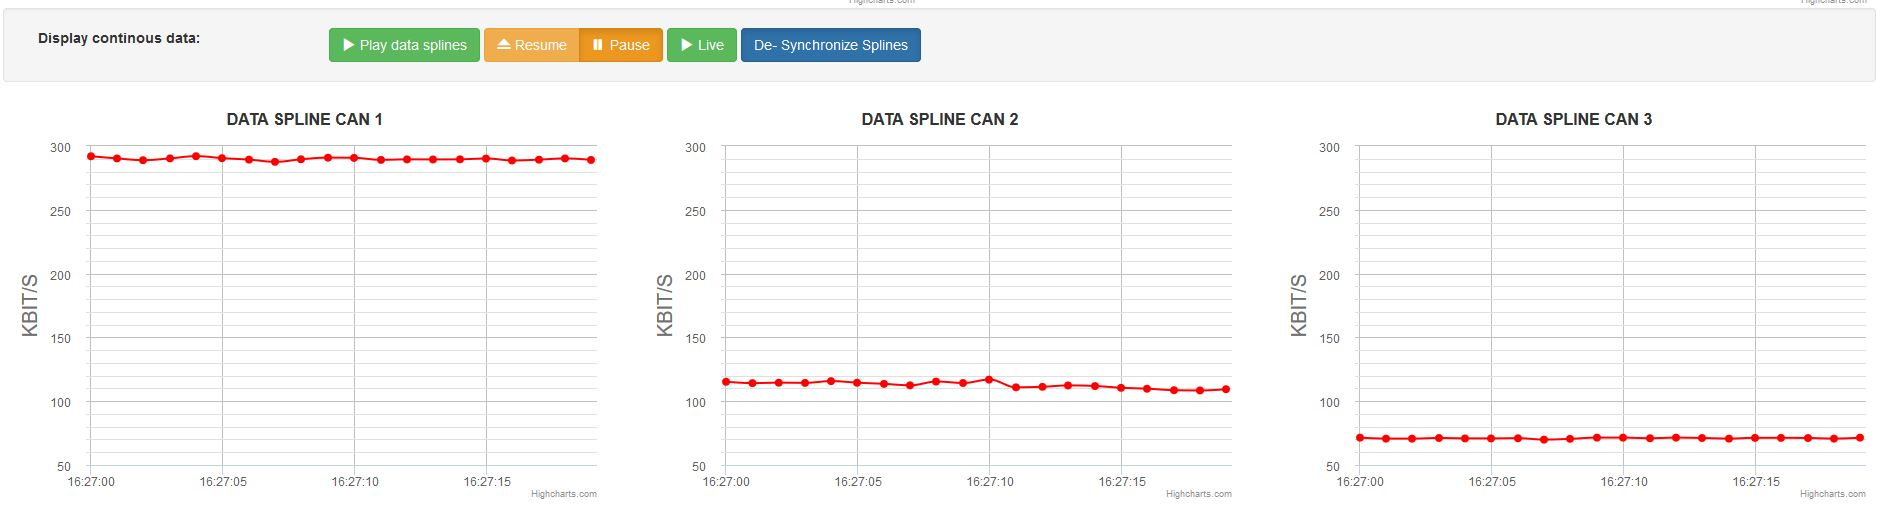
\includegraphics[width=\textwidth]{img/synch_splines}
  \caption{Small Multiples der genutzten Bandbreite von drei verschiedenen CAN-Bussen}
  \label{fig:synch_splines}
\end{figure}

In Burch und Weiskopfs Abhandlung \cite{Burch:2014:FES:2636240.2636839} wird diese Darstellungsform zur Verdeutlichung der Dynamik von Graphen genutzt. Im Small Multiple Aufbau werden Node-Link Diagramme verwendet, welche die Veränderung des Graphen Sequentiell vermitteln soll. Die Vorteile eines Small Multiple Aufbaus gegenüber, von den Autoren als sogenannte Large Singles bezeichnete, einfachen Darstellungen wird in van den Elzen und van Wijks Artikel erläutert \cite{elzen_small_multiple_2013}. Die Kernaussage besagt, dass mit Small Multiples ein breiterer Umfang an Daten aufgenommen werden kann als mit Lage Singles.

\textbf{Index Charts.} Für einige Zeitreihen ist die relative Veränderung ausschlaggebender als die tatsächliche Veränderung der Daten. Für diese Daten kommt ein Index Chart in Frage. Dieser Diagrammtyp zeigt die prozentuale Veränderung für eine Sammlung von Zeitreihen basierend auf einem fixen indexiertem Punkt \cite{heer_tour_2010}. Diese Diagrammart kann beispielsweise bei der Visualisierung von Netzwerkdaten eingesetzt werden um bei einer Verbindungen festzustellen wie sich die Last ab einem bestimmten Zeitpunkt prozentual erhöht. Als Zeitpunkt in einem Fahrzeug beispielsweise das Anlassen des Motors. So lässt sich analysieren welche Verbindungen den größten prozentualen Lastzuwachs, ab diesem Zeitpunkt, erfahren.
% subsection time_series_data_zeitreihen_daten (end)

\subsection{Karten} % (fold)
\label{ssub:karten}
Karten sind von Haus aus der natürliche Weg um geographische Daten darzustellen. Trotzdem eignen auch Sie sich um Netzwerkdaten darzustellen. Viele Geographische Karten werden mit Hilfe eines sogenannten Kartennetzentwurfs entwickelt. Dies ist eine Methode um die dreidimensionale gekrümmte Oberfläche der Erde auf eine zweidimensionale Karte zu übertragen. Es gibt aber auch weitere Kartendarstellungen welche geografische Aspekte von vorn herein abstrahieren oder verwerfen um spezifische Daten hervorzuheben.

\begin{figure}[h]
  \centering
  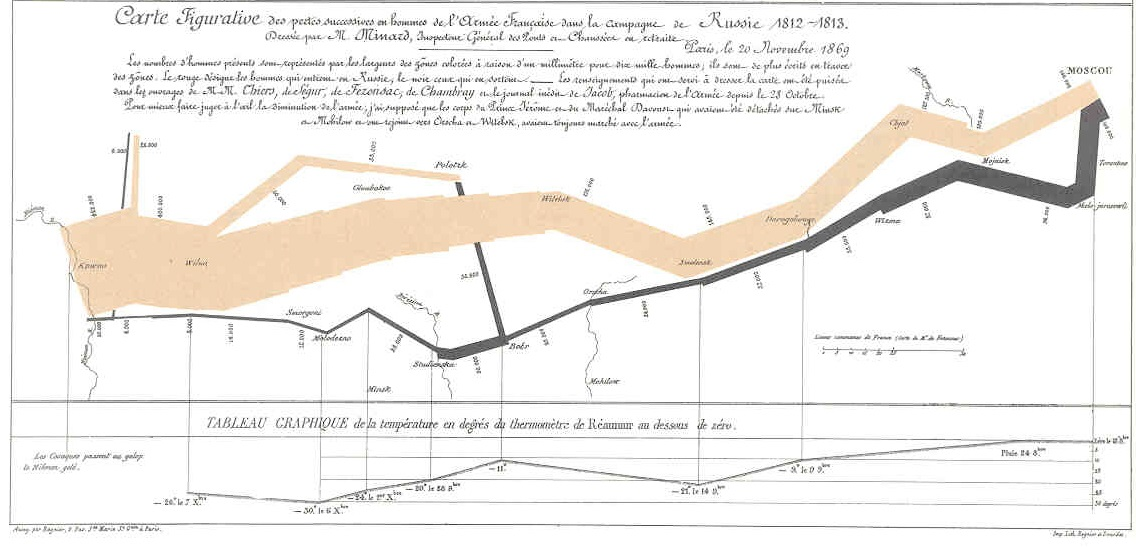
\includegraphics[width=\textwidth]{img/napoleon}
  \caption{Charles Minards Flow Map von Napoleons Russlandfeldzug.}
  \label{fig:nap}
 \end{figure} 
\textbf{Flow Maps.} Eine der wohl bekanntesten Arbeiten dieser Art von Karte ist Charles Minards Grafik über Napoleons Russlandfeldzug (Abbildung \ref{fig:nap}). Eine Flow Map zeigt die Bewegung einer Menge in Raum und Zeit. Für die Darstellung eines Netzwerks, könnte man sich also die Bewegung einer Menge an Datenpaketen (Bandbreite) in Richtung eines Knotens oder Endgerätes vorstellen. 

\textbf{Canonical Map.} Mathematisch wird eine Canonical Map als Morphismus zwischen Objekten beschrieben, welcher aus der Definition der Objekte entsteht. In einer Formel festgehalten: $X \rightarrow X \bmod R $ wobei $R$ eine Äquivalenzrelation aus $X$ ist. Als Beispiel dient hier die Ausarbeitung von Fowler et al. \cite{Fowler:2014:IVN:2671491.2671501}. Diese Arbeit stellt den Internet Traffic auf dem Level der Autonomen Systeme dar. Es wird eine Canonical Map verwendet, welche einer geografischen Karte der Welt ähnelt und den kumulierten IP Traffic mit Hilfe von Heat maps verdeutlicht. Diese Darstellungsart ließe sich für zukünftige Fahrzeugnetze, die in Verbindung mit der Außenwelt stehen werden, adaptieren. So könnte der Traffic aller vernetzten Fahrzeuge aufgezeigt werden, um mögliche Engpässe oder auch Angriffspunkte aufzuzeigen.

\textbf{Choropleth Maps.} Viele Daten werden innerhalb geografischer Grenzen, wie bei Ländern, erfasst. Bei einer Choropleth Karte werden diese Daten über eine Farbkodierung vermittelt. In einem Netzwerk könnten die verschiedenen Elemente (Router, Switches oder Endgeräte) des Netzwerks als Ersatz für ein geografisches Gebiet herhalten um das Datenaufkommen bei diesen Knotenpunkten farblich hervorzuheben. Eine relevante Arbeit in der eine Choropleth-Karte in Verbindung mit einem Netzwerk verwendetet wurde fehlt. Choropleth-Karten kommen allerdings in nahezu jedem Geographischen Informations-System zum Einsatz.
% subsection karten (end)

\subsection{Hierarchische Darstellungen} % (fold)
\label{ssub:hierachische_darstellungen}
Viele Datensätze können schon von ihrem Aufbau her auf hierarchische Weise geordnet werden. Datensätze bestehend aus unter anderem, Ländern, militärischen Kommandostrukturen, Verzeichnisstrukturen oder auch geschichtlichen Ereignissen besitzen hierarchische Merkmale. Es können allerdings auch Daten ohne erkennbare Hierarchie, mit Hilfe von Algorithmen, hierarchisch dargestellt werden. Der k-Means-Algorithmus ist eine solche statistische Methode, welche die Daten empirisch ordnet. 

\textbf{Node-link diagrams.} Eine hervorstechende Art um Hierarchien darzustellen sind Bäume. Eine zweidimensionale Darstellung eines Baumes entspricht einem Node-Link Diagramm. Mittlerweile wurden viele Algorithmen entwickelt um ein Baum-Layout zu schaffen. Der Reingold-Tilford Algorithmus \cite{reingold_tidier_1981} beispielsweise schafft einen sehr engen Baum mit minimaler Platzverschwendung. Dabei entsteht, wie in Abbildung \ref{fig:nodelink} zu sehen, ein radiales Node-Link Diagramm. Ein solches Diagramm wäre natürlich auch für ein Fahrzeugnetzwerk einsetzbar. Mit den Endgeräten als Endknoten und den Routern bzw. Gateways als Elternknoten.

\begin{figure}[htbp]
  \centering
  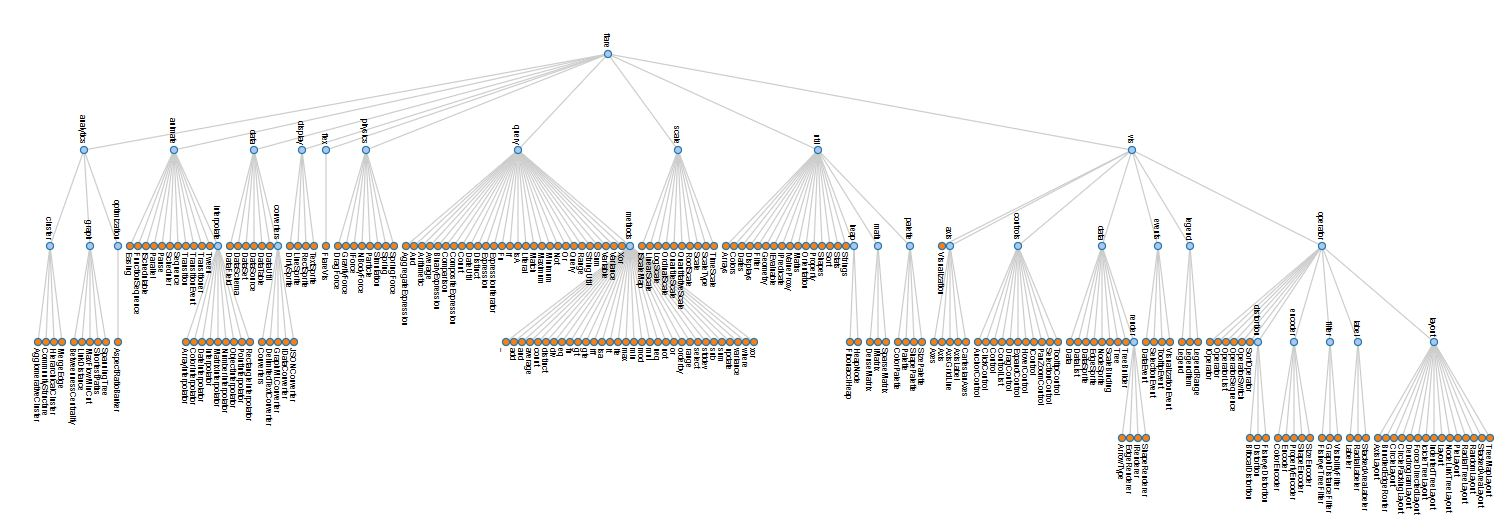
\includegraphics[width=\textwidth]{img/nodelink}
  \caption{Radiales Node-Link Diagramm einer Software-Pakethierarchie. Aus: http://homes.cs.washington.edu/\%7ejheer//files/ \newline zoo/ex/hierarchies/tree.html}
  \label{fig:nodelink}
\end{figure}

\textbf{Adjacency Diagrams.} Die Adjazenzdiagramme stellen eine platzsparende Alternative zu Node-Link Diagrammen dar. Kim und Draper beschäftigen sich in Ihrer Arbeit mit dem Vergleich der beiden dominierenden Darstellungsweisen der Adjazenzdiagramme: Radial und Kartesisch \cite{Kim:2014:RVC:2636240.2636871}. Mit Hilfe einer empirischen Studie und einer Software zur Darstellung der Daten in beiden Formen wird die allgemeine Nutzbarkeit getestet. Diese ist, laut Kim und Draper, allerdings nahezu identisch und eher Kosmetischer Natur. 
Ein Beispiel für eine kartesische Darstellung ist das Icicle Tree Layout. Dieses Layout zeigt die Eltern-Kind Relation per vertikaler Adjazenz, die Kind-Knoten werden direkt unter ihren Eltern angeordnet. Abbildung \ref{fig:icicle} zeigt die gleiche Softwarepaketstruktur wie das vorher behandelte Node-Link Diagrammm. Auch hier ist der Wurzelknoten oben abgebildet, da hier aber die Knoten raumfüllend sind kann die Breite der Knoten zur Darstellung der Größe des jeweiligen Paketes genutzt werden. Dieses zusätzliche Attribut wäre schwer zu realisieren mit einem Node-Link Diagramm.
\begin{figure}[htbp]
  \centering
  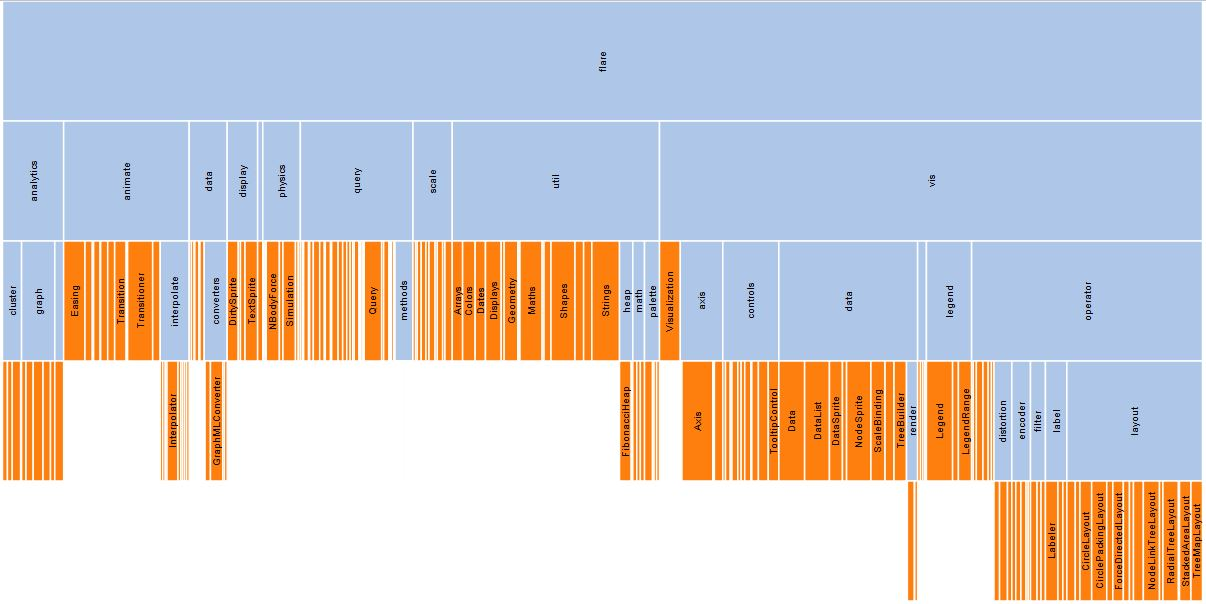
\includegraphics[width=\textwidth]{img/icicle}
  \caption{Vertikal ausgerichtetes Adjazenzdiagramm einer Softwarehierarchie im Icicle Tree Layout. Aus: http://hci.stanford.edu/\%7ejheer/files/ \newline zoo/ex/hierarchies/icicle.html}
  \label{fig:icicle}
 \end{figure} 

\textbf{Enclosure Diagrams.} Im Jahr 1991 entwickelte Shneiderman ebenso platzsparende Diagramme, welche sich der Container- statt der Adjazenzdarstellungsweise bedienen \cite{shneiderman_1991}. Eine Treemap ist ein solches Diagramm. Diese unterteilt rekursiv einen gegebenen Bereich in Rechtecke, so wie bei Adjazenzdiagrammen wird hier die Größe der Knoten leicht sichtbar. Enclosure Diagramme können auch mittels Kreisen anstatt mit Rechtecken aufgebaut werden, als eine Art Venn Diagramm. Diese sind weniger platzsparend, können aber durch den zusätzlich verwendeten Platz die Hierarchie sehr effektiv darstellen. In Abbildung \ref{fig:enclosure} sind neben einer Datei Hierarchie die zwei Diagrammvarianten abgebildet.

\begin{figure}[htbp]
  \centering
  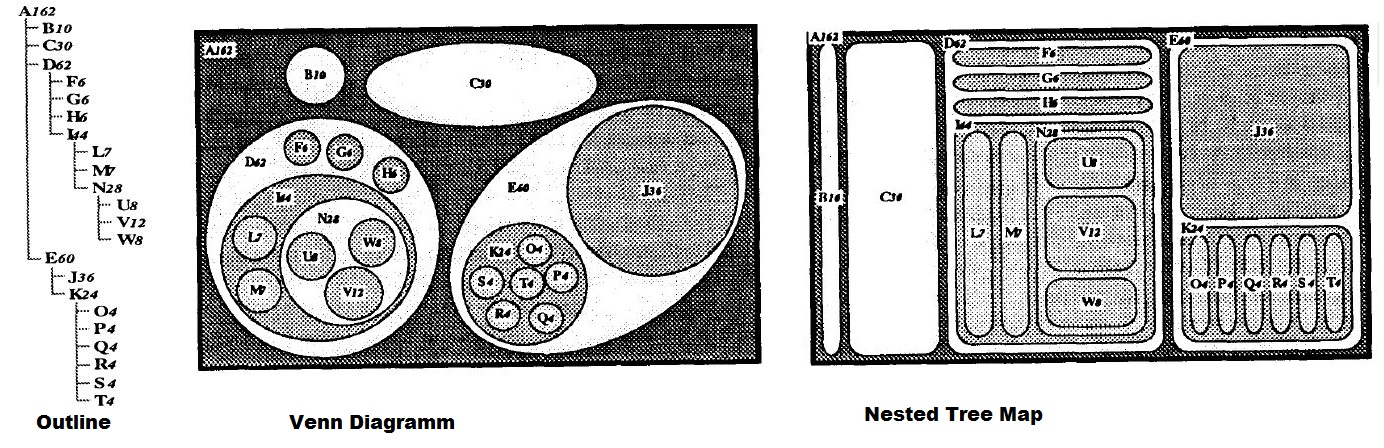
\includegraphics[width=\textwidth]{img/outline}
  \caption{Abbildung einer Datei-Outline mit den entsprechenden Enclosure Diagrammen \cite{shneiderman_1991}.}
  \label{fig:enclosure}
\end{figure}

\subsection{Netzwerke} % (fold)
\label{ssub:netzwerke}
Weitere naheliegende Darstellungsarten sind die der Netzwerkvisualisierungen. In diesen werden Beziehungen zwischen Daten aufgezeigt. Das kann sowohl in sozialen als auch in physischen Netzwerken sinnvoll sein, beispielsweise für die Darstellung der Kommunikation zwischen bestimmten Personen oder respektive die Anzahl der versendeten Pakete zwischen zwei Routern. Datenbanken oder auch Unternehmensstrukturen können ebenfalls von dieser Darstellungsform profitieren, zum einen zum Beispiel zur Visualisierung eines SQL Schemas und zum anderen über die Korrelation von Waren welche von Kunden häufig zusammen gekauft werden. Die Darstellung dieser Informationen wird in Netzwerken mir Hilfe von Knoten welche zu Objekten gehören und Verbindungen (Links) zwischen diesen Knoten welche die Beziehung der Objekte zueinander repräsentieren.  Im mathematischen Sinne sind Netzwerke Graphen. Um einen Graphen darzustellen ist ein effektives Layout von hoher Bedeutung. Typischerweise werden stark verbundene Knoten auch im Bild nah aneinander positioniert, ebenso werden nicht verwandte Knoten weiter voneinander entfernt platziert, um die Beziehungen differenzieren zu können.

\textbf{Force-directed Layout.}  Bei diesem Layout wird der Graph als physisches System modelliert. Knoten sind geladene Partikel welche sich gegenseitig abstoßen, die Verbindungen zwischen diesen fungieren als Federn und halten die Knoten zusammen. Mit Hilfe einer physischen Simulation dieser Kräfte (forces), werden die Positionen der Knoten festgestellt. Hinzu kommt das der Nutzer mittels Interaktivität das Layout ordnen kann wobei die physikalischen Eigenschaften beibehalten werden. Ziel eines Force-directed Layouts ist es die Knoten eines Graphen so in einem zwei- oder dreidimensionealen Raum anzuordnen, dass alle Kanten eine ähnliche länge besitzen und das diese sich sowenig wie möglich überscheniden. Entwickelt wurde dieses Modell von Fruchtermann und Reingold \cite{Fruchterman91graphdrawing}. %\TODO{P 279 in Interactive Data Visualization}

\begin{figure}[htbp]
  \centering
  \includegraphics[width=.5\textwidth]{img/forcedirectedlayout.PNG}
  \caption{Force-directed Layout eines kleinen Beispielnetzwerkes}
  \label{fig:forcedirected}
\end{figure}

\textbf{Matrix View.} Ungerichtete Graphen können mathematisch als Adjazenzmatrix beschrieben werden. Für ein Netzwerk, im Grunde ein ungerichteter Graph, bietet es sich also an eine solche Darstellung zu verwenden. Eine Matrix wird als $N$ mal $N$ Gitter beschrieben, wobei $N$ die Anzahl der Knoten repräsentiert. Jeder Wert in Zeile \textit{i} und Spalte \textit{j} in der Matrix korrespondiert zu der Existenz eines Links von Knoten \textit{i} zu Knoten \textit{j}. Diese werte können binär dargestellt werden oder arber mit einer Gewichtung versehen werden. Ghoniem und Fekete beschreiben in Ihrer Abhandlung die Implementation eines Matrix Views \cite{Ghoniem:2003:MVG:1063669.1063698}. In der Tabelle \ref{tab:matrix2} ist ein Beispielnetzwerk in zwei unterschiedlichen Matrixdarstellungen abgebildet.

\begin{table}[h]
\centering
  \begin{tabular}{*{9}{|c}|}
   & \textbf{a} & \textbf{b} & \textbf{c} & \textbf{d} & \textbf{e} & \textbf{f} & \textbf{g} & \textbf{h} \\[1pt] \hline
   \textbf{a} & & $\bullet$ & $\bullet$ & $\bullet$ & & $\bullet$ & & \\[1pt] \hline
   \textbf{b} & $\bullet$ & & & $\bullet$ & & $\bullet$ & & \\[1pt] \hline
   \textbf{c} &  $\bullet$& & & & $\bullet$ & & $\bullet$ & $\bullet$ \\[1pt] \hline
   \textbf{d} & $\bullet$ & $\bullet$ & & & & $\bullet$ & & \\[1pt] \hline
   \textbf{e} & & & $\bullet$ & & & & $\bullet$ & $\bullet$ \\[1pt] \hline
   \textbf{f} & $\bullet$ & $\bullet$ & & $\bullet$ & & & & \\[1pt] \hline
   \textbf{g} & & & $\bullet$ & & $\bullet$ & & & $\bullet$ \\[1pt] \hline
   \textbf{h} & & & $\bullet$ & & $\bullet$ & & $\bullet$ & \\[1pt] \hline
  \end{tabular}
  \qquad
  \begin{tabular}{*{9}{|c}|}
   & \textbf{p} & \textbf{q} & \textbf{r} & \textbf{s} & \textbf{t} & \textbf{u} & \textbf{v} & \textbf{w} \\[1pt] \hline
   \textbf{p} & & $\bullet$ & $\bullet$ & $\bullet$ & & & & \\[1pt] \hline
   \textbf{q} & $\bullet$ & & $\bullet$ & $\bullet$ & & & & \\[1pt] \hline
   \textbf{r} & $\bullet$ & $\bullet$ & & $\bullet$ & & & & \\[1pt] \hline
   \textbf{s} & $\bullet$ & $\bullet$ & $\bullet$ & & $\bullet$ & & & \\[1pt] \hline
   \textbf{t} & & & & $\bullet$ & & $\bullet$ & $\bullet$ & $\bullet$ \\[1pt] \hline
   \textbf{u} & & & & & $\bullet$ & & $\bullet$ & $\bullet$ \\[1pt] \hline
   \textbf{v} & & & & & $\bullet$ & $\bullet$ & & $\bullet$ \\[1pt] \hline
   \textbf{w} & & & & & $\bullet$ & $\bullet$ & $\bullet$ & \\[1pt] \hline
  \end{tabular}
  \caption{Zwei Matrix-Darstellungen welche den gleichen Graphen abbilden, mit einer unterschiedlichen Anordnung der Knoten. In der rechten Matrix ist die Struktur des Graphen besser ersichtlich. }
    \label{tab:matrix2}
\end{table}
Eine noch detaillierte Einführung in die Netzwerk-Analyse mit Hilfe von Graphen bietet die Arbeit von Brandes et. al \cite{brandes2005network}. %\TODO{Details hier her?}
\ldots
% subsection netzwerke (end)
% Das reicht so ja noch nicht aus um hier mit rein zu kommen, das passt auch gar nicht so hier her. Vielleicht bei der Evaluation der Visualisierungstechniken als einleitung von anderen bereichen
\iffalse %%%%%%%%%%%%%%%%%%%%%%%%%%%%%%%%%%%%%%%%%%%%%%%%%%%%%%%%%%%%%%%%%%%%%%%%%%%%%%%%%%%%%%%%%%%%%%%%%%%%%%%%%%%%%%%%%%%%%%%%%%%%%%%%%%%%%%%%%%%%%%%%%%%%%%%%%%%%%%%%%%%%%%%%
\ldots
Naheliegender angrenzende Bereiche sind jene aus dem Verkehrswesen. In der Flugzeugtechnik wird bereits mit Ethernet im Flugzeugnetz experimentiert und es ist auch schon im Einsatz, beispielsweise im A380 oder der Boeing 787. Auch hier wurde der erhöhte Kommunikationsbedarf erkannt und mit einem auf die Luftfahrt spezialisiertem und von Airbus entwickelten Datennetz reagiert. Das sogenannte Avionics Full-Duplex Switched Ethernet (AFDX) wird hauptsächlich für sicherheitskritische Anwendungen verwendet \cite{steiner_recent_2014}.
\fi      %%%%%%%%%%%%%%%%%%%%%%%%%%%%%%%%%%%%%%%%%%%%%%%%%%%%%%%%%%%%%%%%%%%%%%%%%%%%%%%%%%%%%%%%%%%%%%%%%%%%%%%%%%%%%%%%%%%%%%%%%%%%%%%%%%%%%%%%%%%%%%%%%%%%%%%%%%%%%%%%%%%%%%%%
% section einfuhrung_in_grundlegende_visualisierungen_und_werkzeuge (end)

%%%%%%%%%%%%%%%%%%%%%%%%%%%%%%%%%%%%%%%%%%%%%%%%%%%%%%%%%%%%%%%%%
%%%                         CHAPTER 3                         %%%
%%%%%%%%%%%%%%%%%%%%%%%%%%%%%%%%%%%%%%%%%%%%%%%%%%%%%%%%%%%%%%%%%
\chapter{Anforderungsanalyse} % (fold)
\label{cha:anforderungsanalyse}
Dieses Kapitel widmet sich der Anforderungen an Visualisierungen, sowohl im allgemeinen Sinne, als auch spezifisch für Anforderungen an Visualisierungen für eine Automotive-Netzwerk. Es wird herausgearbeitet was verschiedene Visualisierungstechniken für den Bereich der Fahrzeugnetzanalyse leisten können und welche Daten essentiell für diese Darstellungen sind. Des Weiteren wird analysiert warum spezielle Daten wichtig sind für den Zielbereich. Zur Einleitung wird zunächst auf den Prozess der Erstellung einer Darstellung eingegangen. Der Prozess zur Erstellung einer Visualisierung gibt nicht nur Aufschluss über den Ablauf der Entwicklung sondern auch über dabei entstehenden Anforderungen. Im folgenden wird dieser Prozess beschrieben, welcher auch die Visualization-Pipeline genannt wird \cite{ward_interactive_2010}. 

\begin{figure}[htbp]
  \centering
  \includegraphics[width=\textwidth]{img/visprocess}
  \caption{Ablauf der Entwicklung einer Visualisierung. Frei nach \cite{card_readings_1999}}
  \label{fig:visprocess}
\end{figure}

In Abbildung \ref{fig:visprocess} ist ein Ablauf von den Rohdaten ganz links, bis hin zum Menschen auf der rechten Seite erkennbar. Im Verlauf der Pipeline sind einige Datentransformationen durch Pfeile angedeutet. Diese Pfeile können für mehrere iterative Transformationen stehen. Die Pfeile welche vom User zu den Transformationen führen, bedeuten das der User selbst Anpassungen an diesen Transformationen durchführen kann. 
Zu visualisierende Daten müssen zunächst strukturiert werden um eine Visualisierung überhaupt zu ermöglichen. Die Struktur ist gegeben durch die Namensgebung, den Typ, den Wertebereich und die Semantik eines jeden Datenfeldes oder Attributes. Bekommen Daten eine Struktur, nennt man das auch Datenmodellierung. Nachdem die Daten modelliert wurden müssen nun die relevanten Daten ausgewählt werden. Das herausfiltern der relevanten Daten Teilmengen kann automatisiert werden, mit Algorithmen welche die Eigenschaften der Daten analysieren welche potentiell Interessant sind für den Nutzer. Techniken zur sogenannten Dimensionsreduktion zielen darauf ab nur für die Analyse relevante Dimensionen und deren Relation zueinander in Betracht zu ziehen und zu erfassen. Drei weit verbreitete Algorithmen die eine solche Datenfilterung durchführen werden im folgenden kurz vorgestellt. Self-organizing Maps (SOM) \cite{kohonen_self-organizing_1998} werden dazu genutzt Daten basierend auf ihrer Ähnlichkeit zueinander in einem vordefiniertem Layout zu gruppieren. Die Principal Component Analysis (PCA) \cite{jolliffe_principal_2010} nutzt eine große Anzahl statistischer Variablen und nähert diese einer geringeren Zahl von möglichst aussagekräftigen Linearkombinationen an, wodurch Datensätze strukturiert, vereinfacht und veranschaulicht werden können. Das Multidimensional Scaling (MDS) \cite{borg_modern_2005} versucht die Ähnlichkeit von Daten mittels räumlicher Distanz wiederzugeben. Eine andere Möglichkeit ist die manuelle Variante, in welcher der Nutzer die Daten auswählt. Die Prozesse der Modellierung und der Filterung der Daten sind in Abbildung \ref{fig:visprocess} als Datentransformation zusammengefasst. Sind die relevanten Daten selektiert können diese nun auf grafische Elemente oder Attribute der grafischen Elemente zugeordnet werden. So können verschiedene Komponenten eines Datensatzes verschiedene Attribute beeinflussen, beispielsweise die Größe, Position oder die Farbe. Dieses sogenannte Mapping der Daten schließt meistens eine Verarbeitung der Daten vor dem Abbilden auf die grafischen Elemente ein, wie Skalierung, Filtern oder das Interpolieren der Daten. Darauf folgen einige ästhetische Eingriffe in das Aussehen der Darstellung. Es müssen einige Attribute der Visualisierung festgelegt werden, welche relativ unabhängig von den Daten sind. Dazu gehören die Farbgestaltung, in einigen Fällen die Geräuschwahl und die Belichtung (meist bei 3D Visualisierungen). Im letzten Arbeitsschritt folgt dann die Generierung der Visualisierung. Das Anzeigen der eigentlichen Visualisierung umfasst Schattierung, Textzuordnung und die Darstellung von Linien und meist einheitlich geformte Polygone. dieser Arbeitsschritt wird auch Rendering oder Viewtransformation genannt. Neben der Darstellung der eigentlichen Daten kommen meist noch zusätzliche Informationen zur Unterstüzung des Nutzers Hinzu, diese umfassen zum Beispiel Achsen, Schlüssel sowie Kommentare oder Legenden. 
Der Kern dieses Referenzmodells ist die Abbildung der Datentabellen auf Visuelle Strukturen. Tabellen basieren auf mathematischen Relatinen, visuelle Strukturen hingegen sind darauf Basiert das die grafischen Eigenschaften der Darstellung effektiv von der menschlichen Wahrnehmung verarbeitet werden können. Ohne eine räumliche Komponente sind Daten meist sehr abstrakt und so ist die Transformation über Datentabellen ein wichtiger Zwischenschritt.

Aus dem Wissen der Schritte zur Entwicklung einer Visualisierung aus diesem Abschnitt, leiten sich bereits erste allgemeine Anforderungen für Darstellungen ab. Eine evidente Anforderung ist, aus Daten eine für den User geeignete visuelle Repräsentation zu erzeugen. Die Darstellung muss auf den Endnutzer angepasst sein.

\section{Allgemeine Anforderungen} % (fold)
\label{sec:allgemeine_anforderungen}

Dieser Abschnitt soll die unterschiedlichen Anforderungen welche an Visualisierungswerkzeuge, ebenso wie an Visualisierungstechniken gestellt werden, herausarbeiten. Im folgenden werden dann die essentiellen Anforderungen hervorgehoben um in einem letzten Schritt diese auf ihre Anwendbarkeit im Automotivebereich geprüft. 

Jede Visualisierung fängt bei den Daten an die dargestellt werden sollen. Ein erster Schritt in Richtung der Wahl einer Visualisierung ist die Charakteristika der Daten zu erarbeiten. Daten haben viele Quellen, so können sie von Sensoren oder Software stammen, von Umfragen und Interviews oder auch von Simulationen oder Berechnungen generiert werden. Die Daten können in Ihrer Rohform, also unbehandelt, vorliegen oder die Daten können bereit von den rohen Daten abgeleitet worden sein. Das Ableiten kann beispielsweise durch Prozesse wie Skalierung, Interpolation, Filtern oder Glätten geschehen.  

\subsection{Anforderungen an Visualisierungen} % (fold)
\label{sub:anforderungen_an_visualisierungen}

Damit eine Visualisierung die Bedeutung der ihr zugrundeliegenden Daten transportieren kann, muss diese so Aufgebaut sein das sich dem Nutzer der Sinn erschließt und dieser aufkommenden Fragen nachgehen, Muster entdecken oder Fehler identifizieren und korrigieren kann. Visualisierungen erreichen diese Sinnhaftigkeit durch das Abbilden der Attribute der Daten auf visuelle Eigenschaften. Diese Eigenschaften werden auch die acht visuellen Variablen genannt \cite{ward_interactive_2010} und diese lauten Position, Form, Größe, Helligkeit, Farbe, Orientierung, Struktur und Bewegung. Diese Abbildung der Attribute hilft dem User innerhalb der Daten Muster zu erkennen und interpretieren zu können \cite{card_readings_1999}. Eine einzelne Darstellung kann jedoch nur einige Fragen beantworten, um eine durchdachte visuelle Analyse durchzuführen werden wiederholt neue Views kreiert sowie bestehende exploriert und verbessert. Die Erstellung dieser Views bezieht sich nicht nur auf den Experten, welcher die Visualisierung kreiert sondern auch auf den User der die Views innerhalb eines Visualisierungsprogramms verändert. Durch diesen iterativen Prozess können User Informationen über die Beziehungen der Daten zueinander, kontextabhängige Einflüsse auf Daten und beispielsweise zufällige Muster gewinnen. Dieser Informationsgewinn ist auch das Ziel der Visualisierung, dass Verständnis von Daten zu unterstützen. Visuelle Repräsentationen können kognitive Berechnungen mit Folgerungen aus der Wahrnehmung ersetzen und so das Verständnis, die Erinnerung und die Entscheidungsfindung beschleunigen und verbessern können. Werden Daten mit Hilfe von visuellen Darstellungen zugänglicher und ansprechender gestaltet, eröffnet dies einer breiteren Zielgruppe die Möglichkeit diese zu analysieren und zu untersuchen. Die Schwierigkeit besteht darin effektive sowie anregende Visualisierungen zu erstellen, die gleichzeitig für die vorliegenden Daten geeignet sind.
Das bereits angesprochene Abbilden der Daten spielt dabei eine wichtige Rolle, denn für jeden Datensatz sind die möglichen Kombinationen der visuellen Aufbereitung der Attribute sehr Hoch und damit auch die Anzahl der möglichen Visualisierungsdesigns. Zur Anleitung welche Visuelle Kodierung das Verständnis von Datentypen wie Zahlen, Netzwerke oder Kategorien wurden zahlreiche Studien von Informatikern, Psychologen als auch Statistikern durchgeführt. Von den oben genannten visuellen Variablen eignen sich beispielsweise räumliche Positionsangaben, laut graphischen Wahrnehmungsexperimenten, am besten um numerische Daten in konkreten Visualisierungen festzuhalten \cite{heer_tour_2010}. Bereits 1786 entwickelte William Playfair die noch heute weit verbreiteten, positionskodierten, Balken- und Liniendiagramme \cite{playfair_playfairs_1768}. Die Abbildungen \ref{fig:balken} und \ref{fig:linien} zeigen Beispiele dieser Diagramme. Die Positionsangabe ist laut dieser Experimente gegenüber der Darstellung mit anderen visuellen Variablen klar im Vorteil. 

\begin{figure}[htbp]
  \centering
  \includegraphics[width=\textwidth]{img/balken.png}
  \caption{Ein Balkendiagramm zur Darstellung der genutzten Bandbreite auf verschiedenen Links zu einem bestimmten Zeitpunkt.}
  \label{fig:balken}
\end{figure}

\begin{figure}[htbp]
  \centering
  \includegraphics[width=\textwidth]{img/linien.png}
  \caption{Abbildung eines Liniendiagramms, dass die genutzte Bandbreite auf einem Link über einen vorgegebenen Zeitraum anzeigt}
  \label{fig:linien}
\end{figure}

Zur Visualisierung von, beispielsweise verfügbarer und/oder genutzter Bandbreite auf physikalischen oder virtuellen Links innerhalb eines Netzwerks bieten diese Darstellungen noch immer einen angemessenen Informationsgehalt. Diese gehören weiterhin zu den Standarddarstellungsformen, nicht nur für Netzwerkdaten. Ebenso weit verbreitet ist das, ebenfalls von Playfair entwickelte, Kreisdiagramm (auch als Torten- oder Kuchendiagramm bekannt) zur Darstellung von Teilwerten eines Ganzem zu sehen in Abbildung \ref{fig:kreis}.

\begin{figure}[htbp]
  \centering
  \includegraphics[width=\textwidth]{img/torte.png}
  \caption{Darstellung eines Kreisdiagramms welches die genutzte Bandbreite auf verschiedenen Links anzeigt, als auch die kumulierte verfügbare Bandbreite auf diesen Links.}
  \label{fig:kreis}
\end{figure}

%\TODO{HEATMAPS STATT TORTE? torte schein mir hier etwas zusammenhangslos}

Unter diesen Gesichtspunkten sind allgemeingültige Anforderungen für Visualisierungen kaum festzuhalten. Die Anforderungen Variieren je nach Datensatz, Zielgruppe sowie Umfeld. Zusammenfassend können nur Anforderungen festgehalten werden, welche abstrakterer Natur sind:

\begin{itemize}
  \item Verständlichkeit und schneller Zugriff auf Daten
  \item Zeitersparnis bei der Analyse
  \item Kollaboratives Arbeiten, Zugänglichkeit
  \item Datenabstraktion, Überblick über Daten
\end{itemize}



% subsection anforderungen_an_visualisierungen (end)

\subsection{Anforderungen an Werkzeuge für die visuelle Analyse} % (fold)
\label{sub:anforderungen_an_werkzeuge}
Damit visuelle Analyse Tools effektiv von ihren Usern genutzt werden können, müssen diese eine fließende und flexible Nutzung von Visualisierungen ermöglichen. Um das zu erreichen wird in \cite{heer_interactive_2012} eine \textit{Taxonomy of interactive dynamics for visual analysis} eingeführt. Diese ist in drei Kategorien eingeteilt welche die kritischen Aufgaben der visuellen Analyse beschreiben. Die Kategorien sind \textit{Data and View Specification}, \textit{View Manipulation} sowie \textit{Process and Provenance}. Die erste Kategorie beschäftigt sich mit den spezifischen Daten und Views welche für die jeweiligen Bedürfnisse der Analysten von Interesse sind. Es muss eine Steuerung der Applikation ermöglicht werden, so dass die Daten selektiv visualisiert werden können, irrelevante Daten herausgefiltert werden und ebenso müssen die Informationen sortiert werden können um mögliche Muster erkennbar zu machen. Nach der Erstellung einer Visualisierung muss es den Analysten ermöglicht werden die erstellten Views nach Bedürfnis zu manipulieren, dies beschreibt die zweite Kategorie der Taxonomy. Die Manipulation der Visualisierung ist nötig um Muster aufzeigen zu können, Hypothesen zu untersuchen und zur Navigation in den Daten bspw. via Drilldown. Analyse Tools muss es möglich sein multiple verbundene Visualisierungen zu organisieren und zu koordinieren um mehr Einsicht in Multidimensionale Daten zu bieten als es isolierte Views vermögen. Dies wird schon im häufig zitierten Mantra von Ben Shneiderman vorgegeben: "\textit{Overview first, zoom and filter, then details-on-demand}" \cite{shneiderman_the_eyes_1996}. Die abschließende Kategorie \textit{Process and Provenance} beschreibt den iterativen Prozess der Datenexploration sowie den der Dateninterpretation. Wenn Analysten Ihre bisher getätigten Aktionen innerhalb eines Programms nachverfolgen können kann die Arbeit überprüft und verbessert werden. Es sollte möglich sein die Ergebnisse zu dokumentieren als auch diese mit anderen zu teilen um eine Diskussion darüber zu ermöglichen. Ferner können Analysewerkzeuge auch Anfänger durch Ihre Funktionen führen um die Benutzung und den Einstieg zu erleichtern.
Die vorgegebene Taxonomie bietet einen guten Einstiegs- und Orientierungspunkt in der Welt der Visualisierung und kann ebenso als Checkliste bei der Entwicklung eines neuen Analysetools verwendet werden. Sie zeigt viele Möglichkeiten auf um den Daten Herr werden zu können. Aus dieser Klassifikation für Visuelle Analyse Tools können einige allgemeingültige Anforderungen hergeleitet werden.

\paragraph{Datenexploration ermöglichen} % (fold)
\label{par:datenexploration_ermöglichen}
Es muss dem User ermöglicht werden von einer abstrakteren Sicht auf eine detailliertere Ebne herunter zu navigieren. Diese Steuerung der Anwendung fördert das Erkennen von Mustern und hilft bei der Aufnahme der Informationen, besonders bei großen Datenmengen.
% paragraph datenexploration_ermöglichen (end)

\paragraph{Manipulation und Organisation der Daten ermöglichen} % (fold)
\label{par:manipulation_der_daten_ermöglichen}
Die Datensätze sollten innerhalb einer Visualisierung veränderbar sein. Ermöglicht werden kann dies durch das Setzen von Markern, das Einsetzten von Filtern oder direkte Veränderung von Werten beispielsweise zu Testzwecken. Ebenso sollten die Views in ihrer Repräsentation innerhalb des Tools veränderbar sein, so dass mehrere Views gleichzeitig angezeigt werden können oder Views verbunden werden können für eine verbundene mehrdimensionale Exploration.
% paragraph manipulation_der_daten_ermöglichen (end)
\paragraph{Steuerung und Aufzeichnung der Aktivitäten} % (fold)
\label{par:aufzeichnung_der_aktivitäten}
Für spätere Analysen oder das Teilen der Daten sollten alle Aktivitäten innerhalb des Programms aufgezeichnet werden. Die Möglichkeit erstellte Views und Anmerkungen mit Kollegen zu Teilen sollte ebenfalls mit einbezogen werden. Zudem sollte es bereits vorgefertigte unterstützende Hilfefunktionen geben welche neue Nutzer in das Programm einführen.
% paragraph aufzeichnung_der_aktivitäten (end)
% subsection anforderungen_an_werkzeuge (end)
% section allgemeine_anforderungen (end)

\section{Automotive spezifische Anforderungen} % (fold)
\label{sec:automotive_spezifische_anforderungen}
Im Vorherigen Abschnitt wurden allgemeine Anforderungen an Visualisierungen sowie Analyse Tools herausgearbeitet. Die Anforderungen an eine Darstellung die sich im Bereich der Automotive-Netzwerkvisualisierung bewegt sind wesentlich spezifischer. Es werden zunächst die Daten betrachtet welche Dargestellt werden müssen. Die Daten zur Analyse eines Automotive Ethernet Netzwerks ergeben sich aus verschiedenen Metriken der Netzwerktechnik. Hier stehen diejenigen Metriken, oder auch Kennzahlen, im Vordergrund die hauptsächlich für die Qualität der Verbindung zwischen einem Sender und den Empfängern von Nachrichten genutzt werden. Des Weiteren gibt es \textbf{Systemmetriken}, welche versuchen das System abstrahierter darzustellen und Informationen zu einzelnen Netzknoten bieten. Somit können sie beispielsweise zur Entwicklung einer besseren Topologie eingesetzt werden. Diese Metriken werden im allgemeinen Analysiert um aus den Ergebnissen Designentscheidungen für das Netzwerk zurückzuführen. Ein beispielhaftes Ethernet Netzwerk aus einem Fahrzeug ist in Abbildung \ref{fig:carnet} dargestellt. 
\begin{figure}[htb]
  \begin{center}
    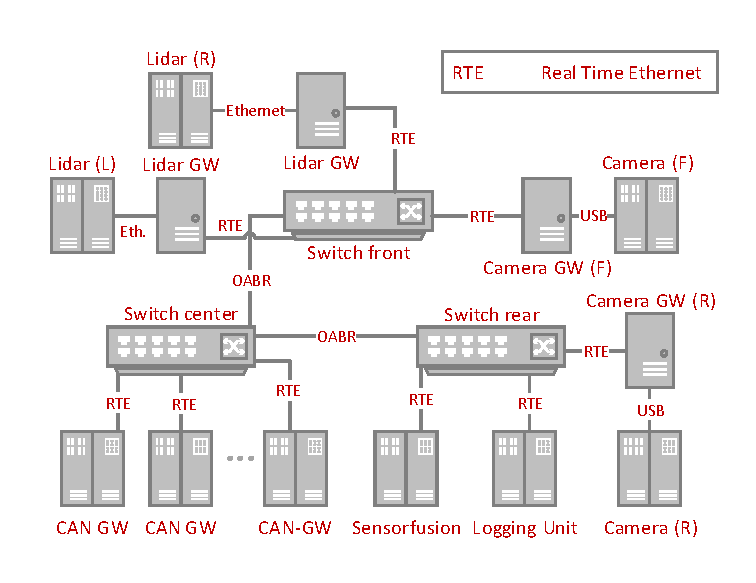
\includegraphics[width=\textwidth]{img/carnet}
  \end{center}
  \caption{Ethernet Backbone Fahrzeugnetz \cite{b-vkaen-15}}
  \label{fig:carnet}
\end{figure}

Nimmt man Metriken als Analysegrundlage für IP gesteuerte Netzwerke, ist die Qualität der Kommunikation hauptsächlich auf die drei Metriken Latenz, Jitter und Paketverlustrate zurück zu führen \cite{kempf_simulationsbasierte_2014} \cite{steinbach_metrik_2011}. Man nennt diese Art der Metriken auch \textbf{Quality of Service Parameter}. QoS Parameter beschreiben die Güte eines Kommunikationsdienstes aus Sicht des Anwenders. QoS Metriken sind zmeist als Anforderungen an ein Netzwerk formuliert, diese soll diese Anforderungen dann umsetzten. Es gibt bei diesen Metriken entscheidende Unterschiede zwischen Simulation und realem Aufbau. Je nach dem wie ein Netzwerk aufgebaut ist können nicht alle diese Metriken nachvollzogen werden. In einer Simulation und beim Debugging für ein Netzwerk ist das Softwaretechnisch gelöst. In der Realität allerdings können hier Probleme Auftreten. Es ist nicht trivial die benötigten Sende- und Empfangszeitpunkte zu erfassen. In einem Testaufbau mit einem Logger, wie in Abbildung \ref{fig:carnet} ist es beispielsweise nicht ohne weiteres möglich. Alle gesendeten Pakete werden dort an den Logger weitergeleitet um diese Analysieren zu können. Die Pakete haben jedoch noch nicht ihr eigentliches Ziel erreicht und deshalb keine Information über den Emfangszeitpunkt gespeichert. Nimmt man als Kompromiss die Empfangszeit am Logger, muss dieser zwingend eine netzsynchronisierte Uhr besitzen damit die Zeiten verleichbar bleiben. Im Folgenden sollen die Quality of Service Parameter näher beschrieben werden. 

\paragraph{Latenz} % (fold)
\label{par:Latenz}
Der Definition nach, ist die Latenz die Verzögerung welche Botschaften von Beginn der Sendung bis zum tatsächlichen Beginn des Empfangs benötigen \cite{reif_automobilelektronik:_2009}. Dieser Parameter dient zur Beschreibung der Performance der angeschlossenen Geräte an ein Netz, denn die Latenz schließt alle Verzögerungen die auf dem Übertragungsweg entstehen können ein und kann gut als Zeitfolge dargestellt werden. Die Latenz kann des Weiteren in drei untergeordnete Metriken gesplittet werden, minimale Latenz, Maximale Latenz sowie durchschnittliche Latenz. Die minimale Latenz beschreibt die geringste Verzögerung die ein Paket zwischen zwei Punkten im Netzwerk benötigt hat. Im Gegensatz dazu steht die maximale Latenz, welche die höchste zeitliche Verzögerung eines Paketes angibt. Die durchschnittliche Latenz ergibt sich aus der mittleren Verzögerung aller Pakete innerhalb eines vorgegebenen Zeitraums.
Die Formel zur Berechnung der Latenz ist:
\begin{equation}
  T_{Receive} - T_{Send}
\end{equation}
 Die Latenz ist eine wichtige Metrik im Automobilnetzwerk. Eine Latenz die konstant und vor allem niedrig, in Relation zum Zeitverhalten der Anwendung, ist beeinflusst die einwandfreien Funktion der angeschlossenen Systeme. 
% paragraph latenz (end)

\paragraph{Jitter} % (fold)
\label{par:jitter}
Wie in \cite{mansour_jitter_2001} beschrieben, ist Jitter die Varianz der Verzögerung von Paketen in Netzwerken. In einem optimalen Netzwerk wären also die Verzögerungszeiten bei identischen Nachrichten immer gleich und die Latenz dadurch immer konstant. Router, Switches und andere Systeme können allerdings durch verschiedene Faktoren die Wartezeiten der Pakete erhöhen. Einige Queueing-Algorithmen welche Prioritäten-basiert arbeiten, können beispielsweise Pakete die über den gleichen Link kommen unterschiedlich bevorzugen. Im Echtzeit-Ethernet Netzwerk welches im Fahrzeugnetz nach Abbildung \ref{fig:carnet} integriert wurde, wird bei bestimmten Nachrichten maximale Verzögerungen von unter $1 \mu s$ gefordert. Eine Einhaltung solcher Vorgaben kann durch so genannte Jitterbuffer erreicht werden. Mit Hilfe dieser Buffer können Pakete länger in Geräten gehalten werden um die Varianz der Laufzeit der Pakete auf einem gleichbleibenden Niveau halten zu können. Das Zeigt das der Jitter ein wichtiger Indikator für ein Fahrzeugnetz ist, beziehungsweise allgemein für jedes elektronische Netzwerk in welchem Daten übertragen werden relevant ist. Jitter wird immer bestimmt über die Laufzeiten zweier Pakete im Bezug zueinander. Zur Berechnung werden die Sende- und Empfangszeitpunkte (Latenzen) beider Pakete benötigt. Zumeist werden zwei aufeinanderfolgende Pakete betrachtet, siehe Formel \ref{eq:jitter1}. Durch die Subtraktion der beiden Laufzeiten erhält man die Varianz zwischen diesen Paketen. Ein Wert nahe null indiziert eine niedrige Varianz. Eine zweite Möglichkeit ist es, alle Pakete mit der Laufzeit eines bestimmten Paketes in Relation zu setzten, zu sehen in Formel \ref{eq:jitter2}. Das kann beispielsweise das Paket mit der bisher geringsten Laufzeit sein.
In einer Formel ausgedrückt: 
\begin{equation}
  |(T_{Receive1} - T_{Send1}) - (T_{Receive2} - T_{Send2})|
  \label{eq:jitter1}
\end{equation}
\begin{equation}
    |(T_{ReceiveMin} - T_{SendMin})  - (T_{ReceiveActual} - T_{SendActual})|
    \label{eq:jitter2}
\end{equation}
% paragraph jitter (end)

\paragraph{Paketverlustrate} % (fold)
\label{par:paketverlustrate}
Die Paketverlustrate (PLR) beschreibt das Verhältnis von gesendeten zu empfangenen Paketen zwichen zwei Engeräten oder auf einzelnen Verbindungswegen. Paketverluste entstehen durch Übertragungsfehler oder zum Beispiel einem überlaufenden Buffer in einem Switch oder Endgerät. Eine Bufferstrategie ist im gefüllten Buffer die am längsten im Buffer vorhandenen Pakete mit den neuesten Paketen zu ersetzen, so dass die älteren verloren gehen. Im Echtzeit Ethernet Netzwerk ist die Paketverlustrate abhängig von der Konfiguration, betrifft aber in erster Linie die Pakete welche keine Echtzeit Anforderungen erfüllen müssen. Paketverluste können allerdings auch durch fehlerhafte Synchronisation, falscher Konfiguration der Empfangszeiträume oder Übertragungsfehler entstehen. Gemessen wird diese Metrik wenn beim Empfänger weniger Pakte ankommen, als ursprünglich gesendet wurden. Die Kennzahl ergibt sich demnach aus 
\begin{equation}
  PLR = \frac{P_{lost}}{P_{send}}
\end{equation}
wobei $P$ die Anzahl der Pakete darstellt. Im Messaufbau mit einem Logger ist die PLR kaum zu erfassen, da es keine Informationen darüber gibt ob ein Paket beim eigentlichen Empfänger angekommen ist oder wie viele Pakete ursprünglich gesendet worden sind. 
% paragraph paketverlustrate (end)

\paragraph{} % dummy for bigger offset

\textbf{Systemmetriken} hingegen liefern keine Informationen über die Qualität des Netzwerkes. Mit einer Systemmetrik lassen sich Schlüsse ziehen und das Netzwerk kann dementsprechend abgeändert werden. Eine Systemmetrik macht keine Aussage über die Qualität eines Dienstes, sondern eher über die damit verbundenen Quality of Service Parameter. QoS Metriken sind also eher relevant aus Sicht der Anwendung und Systemmetriken aus der Sicht des Netzes. Mit diesen Systemmetriken lassen sich Topologien, Routing-Algorithmen und Konfigurationen einzelner Netzelemente bewerten. Relevante Systemmetriken zur Analyse eines Netzwerkes sind beispielsweise die Kapazität, die verfügbare Bandbreite sowie die Linkauslastung. Auch diese sollen in den nächsten drei Passagen beschrieben werden. 

\paragraph{Kapazität} % (fold)
\label{par:kapazitat}
Die maximal mögliche Bandbreite wird als Kapazität beschrieben. Dabei bezieht sich das auf die maximale Bandbreite die auf einem Link oder einem Pfad erreicht werden kann \cite{prasad_bandwidth_2003}. Betrachtet werden die Pakete abzüglich ihrer Header die auf dem gemessenen Layer hinzugefügt werden. Das spielt in IP-Netzen eine große Rolle, da hier der Header bei minimaler Paketgröße relativ groß ist im Verhältnis zum Gesamtpaket. Dadurch ist die Kapazität eines Links bei kleinen Paketen, aufgrund des großen Overheads, geringer. Die Kapazität wird in MB/s angegeben und wird berechnet über die Formel: 
\begin{equation}
  C_{L_3} = C_{L_2} \frac{1}{1+\frac{H_{L_2}}{L_{L_3}}}
\end{equation}
Erarbeitet wurde diese Formel in \cite{prasad_bandwidth_2003}. Wobei $C_{L_x}$ die Kapazität auf dem jeweiligen Layer bestimmt. $H_{L_2}$ ist der Layer-2 Overhead und $L_{L_3}$ bezeichnet die Größe eines Layer-3 IP-Paketes.
% paragraph kapazität (end)

\paragraph{Linkauslastung} % (fold)
\label{par:linkauslastung}
In einem Netzwerk wird die Linkauslastung für jeden Link einzeln gemessen. Sie beschreibt die Auslastung des Links im Verhältnis zur maximalen Bandbreite die pro Zeitintervall zur Verfügung steht. Auch die Linkauslastung wird in MB/s angegeben, kann aber auch in Prozent verdeutlicht werden. Das Intervall beträgt in der Regel eine Sekunde, ist jedoch nicht festgelegt. Wenn innerhalb des Intervalls $0.7$ Sekunden lang übertragen wird, beträgt die Linkauslastung $70\%$. Je kleiner das Intervall gewählt ist, desto besser kann man mögliche Auslastungsspitzen erkennen. Allerdings muss das Intervall messbar bleiben. Dieser Vorteil bei kleinen Intervallen entsteht, da nur wenige Pakete übertragen werden können und diese dementsprechend eine größere Auswirkung auf die Auslastung haben. Berechnet wird die Linkauslastung wie folgt:
\begin{equation}
  \label{eq:5}
  \frac{Sendedauer}{Intervallzeit} \textrm{ oder } \frac{GesendeteDaten}{Intervallzeit}
\end{equation}
\iffalse In Echtzeit-Ethernet Netzen ist besonders die Linkauslastung bezüglich Virtueller Links interessant. Virtuelle Links sind Multicastverbindungen innerhalb des Fahrzeugnetzes, von einem Sender zu mehreren Empfängern. Es wird für jeden Link die Linkauslastung der Virtual Links aufgezeichnet. Bei einem guten Netzdesign, müsste jeder einzelne Link, der sich auf dem Pfad des Virtuellen Links befindet, der Link mit der geringsten Linkauslastung sein.\fi
% paragraph linkauslastung (end)

\paragraph{Verfügbare Bandbreite} % (fold)
\label{par:verfugbare_bandbreite}
Diese bestimmt die, während der Übertragung von Daten, auf einem Link noch zur Verfügung stehende Bandbreite. Somit ist die verfügbare Bandbreite das Gegenstück zur Linkauslastung. Wie beschrieben, misst die Linkauslastung die tatsächlich übertragene Bandbreite, im Gegensatz dazu zeigt die verfügbare Bandbreite die Spanne an welche noch für weitere Anwendungen zur Verfügung steht. Die verfügbare Bandbreite wird in den gleichen Einheiten wie die Linkauslastung angegeben (MB/s oder in Prozent). Wird in einem einsekündigen Intervall die Hälfte der Zeit lang übertragen, ergibt sich eine verfügbare Bandbreite von $50\%$ in dem gewählten Zeitraum. Die verfügbare Bandbreite muss im Bezug auf die maximale Bandbreite gesehen werden, sie berechnet sich also über:
\begin{equation}
  \textrm{Max. Bandbreite des Links } - \textrm{Linkauslastung}
\end{equation}
Zu beachten ist dabei, dass jeder Pfad vom Sender zum Empfänger einen \textit{tight link} besitzt, wessen ungenutzte Bandbreite immer die verfügbare Bandbreite des Pfades (im Fahrzeugnetz bspw. ein Virtueller Link) definiert \cite{hu_evaluation_2003}.
% paragraph verfügbare_bandbreite (end)

\paragraph*{} % dummy for bigger offset
Weitere hier nicht betrachtete Metriken sind beispielsweise die Anzahl Hops im Netzwerk, Buffergröße oder Netwerk-/Topologierobustheit. In dieser Arbeit wurden nur die für Visualisierungen bedeudtsamsten betrachtet. Tabelle \ref{tab:metrik} zeigt alle in diesem Abschnitt näher behandelten Metriken und fasst ihre Eigenschaften zusammen.
\begin{table}[h]
  \begin{tabular}{*{4}{|c}|}
    \textbf{Metrik} & \textbf{Einheit} & \textbf{Formel} \\[2pt] \hline
    Latenz & Sekunden (S) & $T_{Receive} - T_{Send}$ \\[2pt]
    Jitter & Sekunden (S) & $|(T_{Receive1} - T_{Send1}) - (T_{Receive2} - T_{Send2})|$ \\[2pt]
    Paketverlustrate & Prozent (\%) & $PLR = \frac{P_{lost}}{P_{send}}$ \\[2pt]
    Kapazität & MB/s & $C_{L_3} = C_{L_2} \frac{1}{1+\frac{H_{L_2}}{L_{L_3}}}$ \\[10pt]
    Linkauslastung & MB/s oder Prozent (\%) & $\frac{Sendedauer}{Intervallzeit} \textrm{ oder } \frac{GesendeteDaten}{Intervallzeit}$ \\[2pt]
    Verfügbare Bandbreite & MB/s oder Prozent (\%) & $\textrm{Max. Bandbreite des Links } - \textrm{Linkauslastung}$ \\[2pt]
  \end{tabular}
  \caption{Zusammenfassung relevanter Netzwerk Metriken}
    \label{tab:metrik}
\end{table}

Bei der Wahl einer Visualisierung für Metriken, Kennzahlen und Daten kommt es immer auf den jeweiligen Anwendungsfall an. Die Möglichkeiten zur Visualisierung sind sehr vielfältig, weshalb die Wahl eines geeigneten Darstellungsformats entscheidend ist. Die Visualisierung von multiplen Ansichten, Zeitfolgen, Large scale-/Big Data, Netzwerkdaten sowie die Bedeutungsbestimmung von Daten, sind zentrale Themen die für viele Forschungsbereiche relevant sind jedoch noch weiterer Entwicklung bedürfen \cite{isenberg_toward_2014}. Dies sind genau die Themen, welche auch in dieser Arbeit von Interesse sind. Das in Abbildung \ref{fig:carnet}  gezeigte Netzwerk ist in dieser Form auch im Projektfahrzeug der CoRE Gruppe \cite{core_2017} (bzw. des RECBAR Projekts) verbaut gewesen. In Testläufen entstanden bereits bei nur einer Stunde Testzeit enorme Datenmengen. Ungefähr 41,6 Millionen Datensätze entstehen in dieser Zeitspanne, die die Datenbank auf eine Größe von etwa 11 Gigabyte anwachsen lassen. Gerade um dieser Vielzahl an Daten einen Sinn zu verleihen ist eine grafische Aufarbeitung nötig. Auch im Bereich Big Data entsteht bei diesen Datenmengen Handlungsbedarf. Bedenkt man das ein Full-HD Monitor theoretisch maximal etwas über zwei Millionen Datenpunkte anzeigen kann, müssen diese Datenmengen in anderen als den herkömmlichen Visualisierungsarten verarbeitet werden. Einfache Balken und Liniendiagramme reichen in ihrer ursprünglichen Form nicht aus. Ohne Kontext und Visualisierungsformen welche auf die Daten, bzw. den jeweiligen Anwendungsfall, zugeschnittenen sind, sind diese schwer zu interpretieren.
Die eingangs der Arbeit und hier erwähnte steigende Komplexität des Fahrzeugnetzes \iffalse\TODO{In einleitung einfügen}\fi veranlasste Sedlmair et al. zu mehreren Studien über die nötige Visualisierung von Kommunikation innerhalb eines herkömmlichen Fahrzeugnetzwerks \cite{sedlmair2009}\cite{sedlmair_dual-view_2008}. Die genannten Studien beinhalten einige der in Abschnitt \ref{sec:grundlagen_der_evaluation} behandelten Evaluationstechniken mit Nutzerbeteiligung aus den Bereichen der Befragung und den Beobachtungstechniken. Es wurden die Thinking Aloud Methode sowie Fragebögen verwendet. Die Zielgruppe bestand in den Studien ausschließlich aus Fahrzeuganalyseexperten. Durch die steigende Komplexität, wird es auch für Ingenieure immer schwerer Störungen zu analysieren und Diagnosen zu fehlerhaftem Verhalten zu stellen. Es entsteht durchgehend neuer Datenverkehr im Fahrzeug, welcher von speziellen Werkzeugen aufgefangen wird um die Experten zu unterstützen. Jedoch beschreiben diese Tools die Daten hauptsächlich in textueller Form, in dieser Art der Visualisierung fehlt allerdings die Beziehung zwischen Ursache und Wirkung. Um ein tieferes Verständins der Netzwerkommunikation in einem Fahrzeug zu erhalten ist die Anzeige eines zeitlichen Verhältnisses zwischen den Nachrichten notwendig das über einen fortlaufenden Zeitstempel hinaus geht. Zumeist arbeiteten die Experten der Studie nur mit einem Protokoll der versandten Nachrichten innerhalb des Netzwerks, welche nur mit einem Zeitstempel versehen wurden. Ein Datensatz enthält dabei den Inhalt der Nachricht in Reinform sowie einen exakten Zeitstempel als auch Informationen über die ECU welche die Nachricht verschickt hat im Hexadezimalformat. Des Weiteren gibt es zwei Felder welche zum einen automatisch erkannte Fehler anzeigen und zum anderen für manuell erkannte. Im falle der manuellen Erkennung drückt der Testfahrer einen speziellen Knopf im Wagen um den Fehler im Protokoll zu markieren und kommentiert diesen später in der Datei. In Anbetracht das in einem Fahrzeug zur Zeit der Studie ca. 15000 Nachrichten pro Sekunde verschickt werden und das die Protokolle über Wochenenden angefertigt wurden, entstehen Dateien von bis zu 10 GB Größe. Im Vergleich zu eine modernerem Netz wie dem des angesprochenen Projektes in welchem diese Datenmenge bereits nach einer Stunde erreicht wird erscheint der Handlungsbedarf sich hier noch vergrößert zu haben. Interpretiert werden diese Daten mit Tools wie dem Canalyzer\footnote{www.canalyzer.com}. Mit Hilfe dieser Tools können Ingenieure die Fehler lokalisieren und dessen Behebung in Auftrag geben. Allerdings ist die Lokalisierung der Fehler nicht trivial aus mehreren Gründen. 

\begin{itemize}
  \item In den meisten Fällen sind die Fehler welche automatisch von einer ECU erkannt werden, nicht die eigentliche Ursache des Fehlers
  \item Es gibt mehrere Ursachen für Fehlverhalten wie Timingprobleme, Hardwaredefekte oder Nachrichtenverzögerungen
  \item Manuell erfasste Fehler haben eine enorme Verzögerung innerhalb des Protokolls 
\end{itemize}

Das generelle Vorgehen der Experten um einen Fehler auszumachen wird, laut den Studien, schlecht unterstützt. Die genutzten Programme basieren auf Texten und Listen und scheitern daran einen allgemeinen Überblick zu verschaffen und Daten in Zusammenhang zu stellen um mehr Information zu generieren. Die Navigation wird als langsam beschrieben und Datenreduktions oder Big Data Techniken sind nicht vorhanden. Ebenfalls wird die Anzeige von multiplen Ansichten kaum unterstützt und kollaboratives Arbeiten wird gar nicht unterstützt. Alle Studienteilnehmer sprachen sich für eine Verbesserung der Visuellen Aufbereitung der Daten aus. Aus diesen Misständen, als auch den Aussagen der Experten lassen sich einige Anforderungen für Visualisierungen im Automotivebereich ableiten. 

\paragraph{Adäquate visuelle Aufbereitung} % (fold)
\label{par:adaquate_visuelle_aufbereitung}
Es müssen neue Visualisierungstechniken in Betracht gezogen werden und auf ihre Nutzbarkeit im Automotive Umfeld hin evaluiert werden. Detaillierte Listen sind ausreichend für Teile der Aufgaben welche damit verknüpft sind, jedoch muss mit Hilfe von Visualisierungen die Möglichkeit geschaffen werden die Daten zu explorieren sowie Abhängigkeiten und Beziehungen erkennen zu können. 
% paragraph adaquate_visuelle_aufbereitung (end)
\paragraph{Einfacher Zugriff auf Rohdaten} % (fold)
\label{par:einfacher_zugriff_auf_rohdaten}
Daten von Signalen, Nachrichten und Werten müssen leicht und immer erreichbar sein. Datenabstraktion hat viele Vorteile, es muss jedoch auch möglich sein die exakten Inhalte von Nachrichten etc. aufzurufen. Die Darstellung einer Liste sollte ebenso verfügbar sein wie die Möglichkeit Details in abstrakteren Visualisierungen aufzurufen.
% paragraph einfacher_zugriff_auf_rohdaten (end)
\paragraph{Verbesserte Darstellung von Zeitverhältnissen} % (fold)
\label{par:verbesserte_darstellung_von_zeitverhältnissen}
Die Zeitverhältnisse innerhalb einer Liste sind durch dessen Struktur eindeutig vorgegeben. Alle Nachrichten werden nacheinander aufgelistet. Die Navigation in diesen Daten ist jedoch mühsam, es ist lediglich möglich durch Daten zu scrollen und je mehr Datensätze eine Liste vorzuweisen hat, desto Zeitintensiver wird die Navigation. Damit alle Beziehungen zwischen Daten im zeitlichen Sinn erfasst werden können, sind abstraktere sowie detaillierte Zeitinformationen nötig.
% paragraph verbesserte_darstellung_von_zeitverhältnissen (end)
\paragraph{Multiple Ansichten} % (fold)
\label{par:multiple_ansichten}
Die Möglichkeit der Betrachtung zwei oder mehrerer visueller Datenrepräsentationen kann das Verständnis für der komplexen Verbindungen innerhalb von Datensätzen verbessern, deshalb sollte diese Funktionalität in Visuellen Analyse Tools für den Automotivebereich verfügbar sein.
% paragraph multiple_ansichten (end)
% chapter anforderungsanalyse (end)

%%%%%%%%%%%%%%%%%%%%%%%%%%%%%%%%%%%%%%%%%%%%%%%%%%%%%%%%%%%%%%%%%
%%%                         CHAPTER 4                         %%%
%%%%%%%%%%%%%%%%%%%%%%%%%%%%%%%%%%%%%%%%%%%%%%%%%%%%%%%%%%%%%%%%%
\chapter{Evaluationsbasis} % (fold)
\label{cha:evaluationsbasis}
Nachdem in Kapitel \ref{cha:einfuhrung_in_das_umfeld} die Grundlagen der Evaluation und einiger Evaluationstechniken vorgestellt wurden und darauf folgend in Kapitel \ref{cha:anforderungsanalyse} die Anforderungen an eine Visualisierung speziell an eine Visualisierung im Bereich eines modernen Automotive Netzwerks heraus gearbeitet wurden, werden die daraus gewonnenen Erkenntnisse nun kombiniert. Daraus soll hervorgehen, welche Evaluierungstechnik am besten geeignet ist für die Analyse von wissenschaftlichen Arbeiten die sich mit der Visualisierung von und für Daten aus Netzwerken beschäftigen, mit einem Fokus auf den automobilen Bereich. Die eigentliche Analyse der wissenschaftlichen Arbeiten erfolgt dann in Kapitel \ref{cha:evaluation}. Zunächst wird ein Überblick über die Einsetzbarkeit von Evaluationen im Bereich der Visualisierung gegeben und einige Fakten bezüglich der aktuellen Verbreitung verschiedenster Evaluationstechniken in diesem Umfeld aufgearbeitet. Anschließend werden einige Evaluierungstechniken welche mehrfach im Bereich der Visualisierung von Informationen eingesetzt werden betrachtet. Die Techniken werden über die Aufarbeitung mehrerer Metaanalysen erarbeitet.

Von einem historischen Blickwinkel aus betrachtet beschäftigten sich in den letzten 20 Jahren über 80\% der Evaluationen bezüglich Visualisierungen und verwendeter Visualisierungswerkzeuge mit der Bewertung der sich ergebenden Bildern, beispielsweise nach Darstellungsqualität oder Funktionalität, sowie mit der Performance der verwendeten Algorithmen. Allerdings wird in mehr und mehr Evaluationen auf Studien mit Nutzerbeteiligung zurückgegriffen. Von den Teilnehmern dieser Studien wird dann die Leistungen sowie das subjektive Feedback Evaluiert oder es wird ihre (verbesserte) Performance bei der Verwendung der Visualisierung und in der Analyse, als auch bei der Fähigkeit zur Schlussfolgerungen zu ziehen berücksichtigt \cite{isenberg_systematic_2013}. 

Die Wahl der Art der Evaluation ist entscheidend, weil diese vorgibt in welcher Art und Weise die Ergebnisse genutzt werden können. Diese Entscheidung wird von mehreren Faktoren beeinträchtigt. Den Zielen welche mit der Methode erreicht werden sollen, die Umstände und Grenzen die der Evaluationsaufgabe auferlegt sind und der Charakteristik der Objekte welche evaluiert werden sollen. Diese unterschiedlichen Faktoren interagieren miteinander was die Wahl der am meisten geeigneten Evaluationsmethode schwierig gestaltet \cite{kitchenham_evaluating_1996-2}. Die Entscheidung wird zum Abschluss dieses Kapitels getroffen.

\section{Häufig verwendete Evaluationen im Bereich Visualisierung} % (fold)
\label{sec:häufig_verwendete_Evaluationen im Bereich Visualisierung}
In diesem Abschnitt werden einige häufig verwendete Evaluierungsmethoden im Bereich der Visualisierung beleuchtet. Damit ein systematischer Überblick über die Evaluationsmöglichkeiten im Visualisierungsbereich erreicht wird, wurden Meta-Analysen zu Hilfe gezogen. Bei einer Meta-Analyse werden die Ergebnisse mehrerer wissenschaftlicher Studien miteinander verglichen und die Ergebnisse kombiniert. Ziel bei diesen Meta-Analysen ist es die Ergebnisse vergleichbarer wissenschaftlicher Studien zu Betrachten und zu einer möglicherweise allgemein gültigen Aussage zu kommen. Ein wichtiger Nutzen dieser Analysen ist die Aggregation von Informationen, so dass aus statistischer Sicht eine robustere Aussage über die zusammengefassten Ergebnisse der Studien getroffen werden kann. 

Dieser Abschnitt bezieht sich im wesentlichen auf drei dieser Meta-Analysen. Diese Analysen werden in den folgenden Unterabschnitten behandelt, die Abschnitte sind nach dem jeweiligen Titel der Abhandlungen benannt. Innerhalb der Unterabschnitte wird ein Überblick über die betrachteten Evaluationstechniken und die Ergebnisse herausgearbeitet. Die untersuchten Arbeiten sind in ihrer Reihenfolge chronologisch nach ihrem Erscheinungsdatum geordnet.

\subsection{The Challenge of Information Visualisation Evaluation} % (fold)
\label{sub:the_challenge_of_information_visualisation_evaluation}
Die erste hier betrachtete Meta-Analyse stammt aus dem Jahr 2004 und vergleicht die zu dieser Zeit angewandten Praktiken im Bereich der Evaluation von Visualisierungen \cite{plaisant_challenge_2004}. Genannt werden vier Thematisch geordnete Bereiche der Evaluation:

\begin{enumerate}
  \item Kontrollierte Experimente welche Designelemente vergleichen.
  \item Usability Evaluation von Werkzeugen.
  \item Kontrollierte Experimente welche zwei oder mehr Werkzeuge miteinander vergleichen.
  \item Fallstudien mit Werkzeugen in einem realistischem Umfeld.
\end{enumerate}

Catherine Plaisant  sagt in Ihrer Arbeit das die Ergebnisse aus Usabilitystudien und kontrollierten Experimenten sehr hilfreich sind um das Potenzial und die Limitierung der Werkzeuge erkennen zu können. Es müssen allerdings andere Evaluierungsansätze in Betracht gezogen werden, die die explorative Natur von Usern mit einbezieht und welche den Wert dieser Herangehensweise schätzt, dementsprechend angemessen aufbereitet und mit in die Bewertung einbezieht. Es werden im allgemeinen bessere Metriken und Benchmarks um Werkzeuge zu vergleichen vorausgesetzt. Die wissenschaftliche Abhandlung fasst des weiteren derzeitige Evalationspraktiken zusammen und bewertet Herausforderungen die spezifisch für Informationsvisualisierung wichtig sind. Es werden ebenso erste Schritte für die Entwicklung von Benchmarks und verbesserten Evalutionsmethoden und Toolkits bereitgestellt.

Die zu der Zeit des Papers angewandten Praktiken in der Evaluation von Informationsvisualisierungen wurden in dieser Abhandlung mit Hilfe einer weiteren Arbeit \cite{komlodi2004information} in welcher eine Literaturstudie mit über 50 User-Studies durchgeführt wurde herausgefiltert. Daraus haben sich die vier oben genannten Hauptthemen ergeben, welche hier näher beschrieben werden. Der erste Bereich sind Kontrollierte Experimente, welche Designelemente vergleichen. Die Studien dieser Kategorie vergleichen Beispielsweise Widgets wie zB. Slider oder verschiedene Mappings von Informationen auf der grafischen Oberfläche verglichen.
Als zweites wird die Evaluation der Visibility eines Werkzeuges genannt. Studien dieser Richtung geben Feedback über die Probleme die User mit einem Werkzeug haben und zeigen Möglichkeiten auf, wie Designer mit Hilfe dieser Information das Design verbessern können. Ein weiterer Bereich sind Kontrollierte Experimente. Diese Vergleichen allerdings zwei oder mehr Werkzeuge, dabei werden mehrere Werkzeuge verglichen und meistens ist eines dieser Werkzeuge ein neueres, welches mit aktuellen Werkzeugen verglichen wird. Das vierte Evaluationsthema sind Case Studies von Werkzeugen in einer realistischen Umgebung. Diese Studien werden in dem tatsächlichem Umfeld der Nutzer durchgeführt. Die Nutzer werden an reale Aufgaben gesetzt, was die Nutzbarkeit im natürlichen Kontext wiedergeben soll. Ein großer Nachteil dieser Studien ist der Zeitaufwand und besonders das, auch am eigentlichen Arbeitsplatz, die Wirklichkeit nicht leicht zu reproduzieren ist.

Eine Aufgabe die ansteht für die Evaluation von Informationsvisualisierungen ist, dass die Evaluationen auf die realen Aufgaben und Probleme zugeschnitten sind. Damit soll ausgedrückt werden, dass Visualisierungen im Labor natürlich gemessen und getestet werden können, jedoch ist es von Vorteil wenn diese mit Nutzerbeteiligung getestet wird. Ebenso ist es wünschenswert, dass reale Datensätze, in einer für die Anwendung angemessenen Anzahl, verwendet werden und ebenso realistische Aufgaben an die Testuser verteilt werden. Damit User Tests verbessert werden können sollten diese Aufgaben über simple Such- und Lokalisationsaufgaben hinaus gehen und den User mehr fordern. Diese Aufgaben (etwa bewerten, einordnen, kategorisieren o.ä.) sollten im einzelnen bewertet werden, da Werkzeuge für verschiedene Aufgaben eine unterschiedliche Performance haben können. zur zeit der Abhandlung war es gängige Praxis diese Tasks im allgemeinen zu bewerten und nicht nach Ihrem Abschneiden in den einzelnen Disziplinen. Potentiellen Anwendern würde so die Wahl eines Tools für eine spezifische Aufgabe erleichtert.

Mit der konstanten Weiterentwicklung der Visualisierungs-Prototypen in der Forschung, drängen diese auch auf den kommerziellen Markt. Damit diese Werkzeuge eine Nutzen erbringen, müssen bestimmte Features Voraussetzung sein. Dazu gehören das Importieren von Daten, Big Data Kompatibilität, die Möglichkeit für die Nutzer andere Tools im Einklang zu nutzen und das vorhanden sein von Kollaborationsmöglichkeiten mit Anderen. Dies sind Anforderungen die auch heute noch relevant sind.

\TODO{Paper Kernaussage nicht klar?!}

%%\TODO{Was sabbelt die eigentlich nur rum? kann man auch mal schreiben}
% subsection the_challenge_of_information_visualisation_evaluation (end)

\subsection{Empirical Studies in Information Visualisation: Seven Scenarios} % (fold)
\label{sub:empirical_studies_in_information_visualisation_seven_scenarios}
Diese Abarbeitung betrachtet Evaluation aus der Sicht der vorliegenden Szenarien, anstatt aus Sicht des Kategorie der Evaluation. Lam et al. haben in ihrer Ausarbeitung \cite{lam_empirical_2012} 850 Paper hinsichtlich möglicher Evaluierungsszenarien untersucht. Die sieben erarbeiteten Szenarien zeigen den Stand der Evaluationspraktiken der untersuchten Arbeiten. Die Dokumente stammen aus den Konferenzen der VAST-Reihe, EuroVis, InfoVis und dem IVS Journal. In den 850 Abhandlungen fanden sich in 361 Abhandlungen welche eine Evaluation enthielten. Sie haben sieben verschiedene Szenarien ermittelt, welche sich in zwei grundlegende Kategorien aufteilen. Zum einen gibt es Szenarien, welche mit dem Verständnis der eigentlichen Visualisierungen beschäftigen, zum anderen solche die zum Nachvollziehen der Datenanalyse dienen. 
Die Szenarien zum besseren Verständnis der Datenanalyse sind:

\begin{itemize}
  \item Understanding environments and work practices (UWP)
  \item Evaluating visual data analysis and reasoning (VDAR)
  \item Evaluating communication through visualization (CTV)
  \item Evaluating collaborative data analysis (CDA)
\end{itemize}

Die Szenarien zum besseren Verständnis der Visualisierungen sind:

\begin{itemize}
  \item Evaluating user performance (UP)
  \item Evaluating user experience (UE)
  \item evaluating visualization algorithms (VA)
\end{itemize}

Ziel dieser Abhandlung von Lam et al. ist es einen Überblick über die verschiedenen Evaluierungsszenarien zu geben und für die Praxis eine Entscheidungshilfe zu offerieren so dass die richtigen Evaluationsziele gesetzt, die richtigen Fragen gestellt und eine Vielzahl methodischer Alternativen für diese Fragen und Ziele gegeben werden können. Weiterhin soll die Arbeit eine durch die szenariobasierte Gliederung die Wahl spezifischer Evaluationsziele vor der Betrachtung einzelner Methoden fördern. Ebenso werden vielfältige Methoden für jedes Szenario vorgestellt und mit Hilfe von Beispielen, auch aus angrenzenden Disziplinen, untermauert. Die Arbeit soll als ein erster Schritt in Richtung eines Repositorys für Beispiele und Szenarien als Referenzen dienen. 

Diese sieben Szenarien repräsentieren Kategorien von Evaluationen welche die Autoren durch eine Literaturanalyse erarbeitet haben. Für jedes Szenario sind die Ziele und Resultate, Fragen an die Evaluierung so wie Beispiele und Methoden festgehalten. In den folgenden Absätzen sollen die genannten Szenarien näher Beschrieben werden.

\paragraph{UWP} % (fold)
\label{par:uwp}
Evaluationen in diesem Bereich eruieren formale Anforderungen an das Design. Das Ziel der Evaluation der Informationsvisualisierung in dieser Kategorie ist das Verständnis der Abseitsweise, Analyse oder der Art der Informationsverarbeitung einer Gruppe von Menschen. Als Ergebnis erhält an meist Schlussfolgerungen für das Design basierend auf einem holistischem Verständnisses der derzeitigen Arbeitsabläufen und Praktiken, dem Zustand des Arbeitsumfeldes an sich und derzeit verwendeter Werkzeuge. Evaluationsfragen in diesem Bereich zielen auf die Identifizierung bestimmter Features ab, welche die Visualisierung besitzen sollte.
Mögliche Methoden die in diesem Umfeld eingesetzt werden können beziehen sich meist auf qualitative Daten aus Interviews oder Daten aufgrundlage von Beobachtungen. Beispiele für diese Methoden sind \hyperref[ssub:techniken_auf_grundlage_von_beobachtungen]{Beobachtungen des Arbeitsumfeldes, Beobachtungen im Labor} oder auch \nameref{par:interviews}. In Abschnitt \ref{ssub:techniken_auf_grundlage_von_beobachtungen} sind diese Evaluationstechniken mit Nutzerbeteiligung näher beschrieben. 
% paragraph uwp (end)

\paragraph{VDAR} % (fold)
\label{par:vdar}
Im Bereich VDAR studieren Evaluationen ob und wie Visualisierungswerkzeuge die Generierung von relevanten und anwendbarem Wissen in einem Bereich fördern. VDAR Evaluationen werden meist auf bereits weit entwickelte Software angewandt. Ein Hauptziel der VDAR Evaluationen ist es zu Bewerten in wie fern eine Visualisierungssoftware den Nutzer in der visuellen Analyse unterstützt und damit auch in der Fähigkeit Schlussfolgerungen aus den Daten ziehen zu können. Die Ergebnisse solcher Evaluationen können quantitativer Natur sein, wie die Anzahl der gewonnenen Einsichten während einer Testanalyse oder subjektives Feedback, wie gesammelte Meinungen über die Qualität der Möglichkeiten zur visuellen Analyse. Fragen an eine Evaluation aus dem VDAR Umfeld beschäftigen sich hauptsächlich damit wie gut ein Werkzeug bestimmte Aspekte der visuellen Analyse unterstützt. Methoden welche bei einer VDAR Evaluation eingesetzt werden sind \hyperref[ssub:techniken_auf_grundlage_von_beobachtungen]{Fallstudien, Beobachtungen unter Laborbedingungen}, \nameref{par:interviews} und \hyperref[ssub:empirische_techniken_auf_grundlage_von_experimenten]{kontrollierte Experimente}. Alle genannten Methoden sind in Abschnitt \ref{sub:evaluationstechniken_mit_nutzerbeteiligung} nachzulesen.
% paragraph vdar (end)

\paragraph{CTV} % (fold)
\label{par:ctv}
Evaluierungen aus der Gruppe der Communication Through Visualization behandeln die Frage wie und ob Kommunikation von der Visualisierung unterstützt wird. Mit Kommunikation sind hier mehrere Aspekte wie Lernen, Lehren oder Präsentieren. In diesem Szenario haben Visualisierungen meist das Ziel dem Nutzer eine gewisse Nachricht zu überbringen, im Gegensatz zur Datenexploration oder der Datenermittlung. Die zugehörige Evaluation versucht dann zu bemessen wie effektiv eine solche Nachricht übermittelt und angenommen wird. Ein Beispiel für eine Nachricht dieser Art sind Umgebungs- bzw. Ambientdisplays. Diese Displays sollen meist eine schnelle Kommunikation mit vorbeigehenden Menschen ermöglichen. Studien in CTV versuchen die Qualität einer Software mit Hilfe von quantitativen Metriken wie Lerngeschwindigkeit, Bindung des Nutzers mit den angezeigten Informationen und Exaktheit der Informationen oder mit qualitativen Metriken wie Interaktionsmuster davon wie Nutzer mit dem Display arbeiten und die Informationen absorbieren. Aufgrund dieser Metriken beziehen sich zu stellende Fragen für dieses Evaluationszenario hauptsächlich auf die Interaktion und Kommunikation mit der Visualisierung. Methoden die in diesem Bereich häufig eingesetzt werden sind \hyperref[ssub:empirische_techniken_auf_grundlage_von_experimenten]{Experimente}, \nameref{par:interviews} und \hyperref[sub:evaluationstechniken_mit_nutzerbeteiligung]{Beobachtungen im Feld}. Diese Evaluationsthemen wurden in Abschnitt \ref{sub:evaluationstechniken_mit_nutzerbeteiligung} behandelt.
% paragraph ctv (end)

\paragraph{CDA} % (fold)
\label{par:cda}
Das Szenario CDA betrachten Evaluationen ob ein Werkzeug für Kollaboration, kollaborative Analyse und kollaborative Entscheidungsprozesse unterstützt. Die meisten Evaluationen in diesem Bereich Zielen darauf ab ein ganzheitliches Verständnis der Gruppenarbeitsprozesse der Kollaborativen Werkzeuge zu erlangen um davon Konsequenzen für das Design abzuleiten. Eine Evaluation im CDA Bereich beschäftigt sich hauptsächlich mit Fragen wie gut ein System kollaboratives Arbeiten unterstützt, wie mit dem System kollaborativ gearbeitet werden kann und ebenso ob Kommunikation zwischen den Kollaborateuren stattfinden kann. Evaluationsmethoden aus diesem Szenario sind beispielsweise \hyperref[par:cooperative_evaluation]{Heuristische Evaluation, Loganalyse sowie Feld- und Laborbeobachtungen}, näher beschrieben in Abschnitt \ref{ssub:heuristische_evaluation}.
 % paragraph cda (end)

 \paragraph{UP} % (fold)
 \label{par:up}
 User Performance Evaluationen wollen ermitteln wie sich bestimmte Features auf die objektiv messbare User Performance auswirken. Objektive Metriken in diesem Bereich sind Zeitersparnis und die Fehlerrate. Es ist ebenfalls möglich eine subjektive Leistungssteigerung festzustellen, wie die Qualität der erbrachten Arbeit, solange die Metriken objektiv bewertet werden können. Erwartbare Ergebnisse einer Evaluation aus diesem Umfeld sind zumeist numerische Werte welche durch die Analyse beschreibender Statistiken, wie Median, Mittelwert oder Standartabweichung, ermittelt werden. Die Fragestellung in diesem Bereich kann im Grunde auf zwei Typen heruntergebrochen werden. Zum einen wie eine Visualisierung oder die Interaktion mit einer Visualisierung mit einer anderen auf Basis von der menschlichen Performance verglichen werden kann und zum anderen was die Beschränkungen der visuellen Wahrnehmung des Menschen für visuelle und interaktive Umsetzungen sind. Zur Beantwortung dieser Fragen werden meist \hyperref[ssub:empirische_techniken_auf_grundlage_von_experimenten]{kontrollierte Experimente} oder Loggings aus dem \nameref{par:thinking_aloud} Bereich, behandelt in Abschnitt \ref{par:thinking_aloud}.
 % paragraph up (end)

 \paragraph{UE} % (fold)
 \label{par:ue}
 Im Bereich der User Experience wird das subjektive Feedback und die Meinung der Nutzer ausgewertete. Evaluationen der User Experience versuchen ein Verständnis davon zu erreichen wie Nutzer auf eine Visualisierung reagieren. Das Ziel dabei ist die Reaktionen der Nutzer auf die Visualisierung zu sammeln und diese Informationen im Design, eine zukünftigen oder grade im Entwicklungsprozess befindlichen Visualisierung, zu berücksichtigen. Die gewonnenen Daten können von Designern genutzt werden um Funktionslücken und mögliche Designfehler zu entdecken. Die Kernfrage der User Experience Evaluationen ist: Was hält meine angestrebte Zielgruppe von der ihr vorliegenden Visualisierung? Detaillierter ausgedrückt, sind damit die verschiedenen Features einer Visualisierung oder eines Systems gemeint und welche davon am besten angenommen werden, welche und wie diese verbessert werden können und ob sie im allgemeinen leicht zu verstehen sind. Damit diese Fragen zu genüge beantwortete werden können bedient sich das UE Szenario mehrerer Methoden, darunter Usability Tests aus dem Bereich der \nameref{ssub:heuristische_evaluation} wie in Abschnitt \ref{sub:evaluationstechniken_basierend_auf_expertenanalyse} beschrieben. Ebenso sind \hyperref[ssub:techniken_auf_grundlage_von_beobachtungen]{Beobachtungen im Feld} und \nameref{par:fragebögen} oft genutzte Methoden. Diese Methoden wurden in Abschnitt \ref{sub:evaluationstechniken_mit_nutzerbeteiligung} des zweiten Kapitels beschrieben.
 % paragraph ue (end)

 \paragraph{VA} % (fold)
 \label{par:va}
 Evaluationen in Bereich der Visualization Algorithms liegt der Fokus auf der Performance und Qualität der Visualisierungsalgorithmen, basierend auf dem generierten Output. Ein Visualisierungsalgorithmus ist im wesentlichen definiert als ein Prozess welcher die visuelle Darstellung von Informationen optimiert, gemäß eines vorgegebenen Visualisierungszieles. Evaluationen von Visualisierungsalgorithmen wollen zeigen wie ein gewählter Algorithmus im Vergleich zu seinen Alternativen abschneidet und die Grenzen des Algorithmus, in Form von Datenmenge, Komplexität und Grenzwerten, austesten. Bemessen wird die Performance in Rechenleistung und die Qualität der Visualisierung wird anhand von Metriken, wie dem schnelleren Erkennen von Zusammenhängen, bestimmt. Die Fragen welche eine Evaluierung im VA Bereich aufwirft, beschäftigen sich hauptsächlich mit der Effektivität der visuellen Darstellungen und der Recheneffizienz mit welcher die daten aufbereitet werden. Die zur Beantwortung dieser Fragen eingesetzten Methoden sind Qualitätsbewertung der Visualisierung die Analyse der Algorithmusperformance, diese Techniken sind dem Bereich \ref{sub:evaluationstechniken_basierend_auf_expertenanalyse} \nameref{sub:evaluationstechniken_basierend_auf_expertenanalyse} zuzuordnen. 
 % paragraph va (end)
\iffalse Besonders das Szenario aus der Datenanalyse \textbf{evaluating visual data analysis and reasoning (VDAR)} sticht für die angestrebte Arbeit heraus. Evaluationen in diesem Bereich fokussieren sich hauptsächlich darauf ob und wie ein Visualisierungswerkzeug visuelle Analysen und Schlussfolgerungen über Daten zulässt. Mögliche Ergebnisse sind hierbei sowohl Metriken (bspw. Anzahl der Analyseerkenntnisse), als auch subjektives Feedback (bspw. Umfrage über Datenanalysequalität). Meist werden in diesem Bereich Feldstudien genutzt, häufig in der Form von Fallstudien 
\fi

\begin{figure}[htbp]
  \centering
  \includegraphics[width=\textwidth]{img/prozente_vis_lam.pdf}
  \caption{Jedes Jahr zeigt die prozentuale Anzahl der Szenarien die in diesem im Schnitt pro Konferenz vorgestellt wurden.}
  \label{fig:szenarien}
\end{figure}

Die Szenarien der Arbeit von Lam et al. zeigen die weite Spanne von Evaluationszielen und -fragen mit der sich im Bereich der Informationsvisualisierung beschäftigt wird. Die Autoren beschreiben diese Diversität als einen Trend für Evaluationen von Visualisierungen, wie Abbildung \ref{fig:szenarien} zeigt werden nicht nur unterschiedlichen Ansätze mehr sondern ebenfalls die Anzahl der Arbeiten welche eine Evaluation beinhalten. Das größte Interesse liegt dabei bei den Evaluationen der Szenarien aus dem Bereich zum besserem Verständnis der Visualisierungen. Diese drei Szenarien, Evaluating User Performance (33 Prozent), Evaluating User Experience (34 Prozent) und Evaluating Visualization Algorithms (22 Prozent) decken 89 Prozent aller Arbeiten mit Evaluationen ab. Dies steht in großem Kontrast zu dem nur 11 prozentigem Anteil der Evaluationen zum besseren Verständnis der Datenanalyse und Prozesse. Dieser Anteil erscheint etwas gering, obwohl aus diesem Bereich wichtige Fragestellungen für Visualisierungen stammen. In VDAR zum Beispiel wie Datenexploration oder Data Mining unterstützt werden. Als mögliche Gründe für diesen Gegensatz werden Tradition, Langwierigkeit der Methoden und qualitative statt quantitativer Ergebnisse genannt. 

Der Fokus dieser Arbeit liegt mehr auf den Zielen und Ergebnissen welche Evaluationen hervorbringen sollen, statt auf die Methoden an sich. Durch diese Aufteilung ist es möglich Fragen an die eigene Evaluation zu stellen und so eine Mehrzahl an Methoden aufgezeigt zu bekommen, als auch einen Ansatzpunkt für mögliche neue Evaluationstechniken. Indem mehrere Methoden in verschiedenen Szenarien vorgeschlagen werden, zeigt sich das nicht eine Evaluationsmethode vollständig ein gesamtes Szenario untersuchen kann. 

Da sich Lam et al. allerdings auf den von ihnen als Informationsvisualisierung bezeichneten Bereich beschränken ist kein vollständiges Bild der Evaluationspraktiken für Visualisierungen gegeben. Es gibt einen weiteren großen Bereich welcher als Wissenschaftliche Visualisierungen bezeichnet wird. In dem folgenden Unterabschnitt wird auch dieser Aspekt berücksichtigt. 
% subsection empirical_studies_in_information_visualisation_seven_scenarios (end)

\subsection{A Systematic review on the Practice of Evaluating Visualisation} % (fold)
\label{sub:a_systematic_review_on_the_practice_of_evaluating_visualisation}
Die Arbeit von Isenberg et al. \cite{isenberg_systematic_2013} baut Thematisch auf der von Lam et al. auf \cite{lam_empirical_2012} und bedient sich auch der Terminologie der dort vorgestellten Szenarien. In der Abhandlung \textit{A Systematic review on the Practice of Evaluating Visualization} wird ein Rückblick auf auf die Entwicklung der Evaluationspraktiken der Arbeiten aus der IEEE Visualization Konferenz genommen. Das Ziel besteht darin dem Leser einen ganzheitlichen Überblick über Evaluationen im Bereich der Visualisierung zu liefern und die allgemeinen Ziele von Evaluationen zu zeigen sowie diese mit den Zielen der Arbeiten mit Evaluationen aus der IEEE Visualization Konferenz zu vergleichen. War das Ziel von Lam et al. noch die Szenarios zu kreieren und einen Überblick über die Informationsvisualisierung zu geben, so fokussiert sich die Arbeit von Isenbert et al. darauf auch den Teil der sogenannten wissenschaftlichen Visualisierungen abzudecken. Es gibt demnach grundlegend zwei verschiedene Evaluationsrichtungen aus denen Visualisierungsevaluationen entstehen. Zum einen wissenschaftliche Evaluationen und zum anderen Design Evaluationen. Wissenschaftler versuchen ein repräsentatives Modell anhand einer Evaluation zu bestimmen, während Designer ein Werkzeug oder eine Darstellung verbessern wollen. Die wissenschaftliche Seite beschäftigt sich mit der Validierung der Modelle und der Reproduzierbarkeit innerhalb dieser. Für den Designer liegt der Fokus eher auf dem User, also auf Aspekten wie der Funktionalität, Usability und der Ästhetik.

Um ein systematischen Überblick über den Stand der Evaluationen in Visualisierungsbereich zu erhalten haben Isenberg et al. eine qualitative Literaturanalyse durchgeführt. Diesen Überblick haben sie mit Arbeiten aus der IEEE Visualization Konferenz, die mittlerweile IEEE Scientific Viusalization Konferenz heißt, erstellt und mit den Ergebnissen von Lam et al. aus der IEEE Information Visualization Konferenz verglichen. 

Wie von Lam et. al eingeführt wurden Evaluationsszenarien zur Einordnung der Evaluationen genutzt. Isenberg et al. haben von den von Lam et al. vorgegebenen Szenarien jedoch eines leicht abgeändert und die Szenarien um ein weiteres ergänzt. Die zwei neuen Szenarien werden im folgenden vorgestellt.

\paragraph{Algorithm Performance (AP)} % (fold)
\label{par:algorithm_performance_}
Vorher durch Lam et al. als Visualization Algorithms veröffentlicht, haben die Autoren der Arbeit dieses Abschnitts dieses Szenario umbenannt um den von Ihnen gefundenen Ergebnissen gerechter zu werden. In diesem Szenario fanden sich 35\% aller untersuchten Evaluationen wieder. Evaluationen dieser Kategorie versuchen mit einem quantitativen Ansatz die Performance oder Qualität von Visualisierungsalgorithmen zu bestimmen. Die Performance oder Qualität wird zum Beispiel durch die Messung der Renderinggeschwindigkeit in Frames per Second (FPS) oder der Rechenperformance in Rechenzeit bestimmt. Durch die Bestimmung solcher Metriken können die mögliche maximale Größe von Datensätzen auf der gegebenen Plattform mit dem gegebenen Werkzeug bestimmt werden. Weitere gefundene Metriken zur Evaluation einer Visualisierungstechnik oder Implementation sind solche die die Qualität eines Visualisierungsalgorithmusses quantitativ bestimmen. Das Ziel dabei ist zu messen was ein Nutzer sehen kann und dies zu bewerten ohne das Nutzer beobachtet werden müssen. Bei einem Netzwerkgraphen beispielsweise werden die Anzahl der Überschneidungen der Verbindungen als eine Kennzahl für die Verständlichkeit herangezogen. 
\iffalse
NOCH AN DIESER STELLE RELEVANT?

For the visualization literature we
analyzed,  this subset of AP evaluations included,  for example,  the
reporting of compression rates for shape compression techniques or
error metrics for the generated visuals. Such objective metrics to assess
a technique or its produced results was typically provided when some
kind of ground truth or other established quality standards (visual and
otherwise) existed against which results could be compared.

, typical
evaluations gave rendering speeds for a number of different example
datasets and reported the used platform.  Good evaluations analyzed
the behavior for a range of dataset sizes or used a number of additional
metrics to assess different concepts of visual quality of the results. A
good performance analysis was presented, for instance, by Lindstrom
and Isenburg [39]; a nice example of objectively analyzing the quality
of a proposed visualization result is Schultz and Seidel’s work [57
\fi
Typische Evaluationen in diesem Szenario sind im Bereich der \nameref{sub:evaluationstechniken_basierend_auf_expertenanalyse}, welche in Abschnitt \ref{sub:evaluationstechniken_basierend_auf_expertenanalyse} besprochen wurden, angesiedelt.

% paragraph algorithm_performance_ (end)
\paragraph{Qualitative Result Inspection (QRI)} % (fold)
\label{par:qualitative_result_inspection_}
Dieses Szenario wurde gänzlich neu von den Autoren entwickelt, denn ein Großteil der untersuchten Arbeiten passte nicht in die vorgegebenen sieben Szenarien. QRI gehört zur Kategorie zum Verständnis von Visualisierungen, 95\% aller untersuchten Evaluationen fallen in dieser Arbeit in diese Kategorie. Evaluationen dieser Kategorie bewerten die Ergebnisse von Visualisierungen und Darstellungen. Im Gegensatz zum User Experience Szenario sind hier keine Nutzer involviert, stattdessen führt derjenige der sich mit der Ergebnisdarstellung beschäftigt die Bewertung selbst durch. Die Evaluation bekräftigt den Leser darin mit dem in der Arbeit gewonnenen Ergebnissen übereinzustimmen indem dieser die Resultate der Evaluation untersucht. Ein Beispiel für einen solchen Fall ist der Satz: \textit{\glqq Die Abbildung zeigt das dieses Werkzeug die Struktur x aus den vorliegenden Daten klar darstellen kann, was mit dem vorherigen Ansatz nicht möglich war.\grqq} 

Insgesamt fanden die Autoren drei wichtige Evaluationstypen in diesem Szenario:

\begin{enumerate}
  \item Evaluation der Qualität der Darstellungen welche ein Algorithmus produziert hat. Dabei ist das Ziel das ein neu entwickelter Algorithmus eine bestimmte Qualität erreicht und darauf folgend bewertet und gezeigt wird wie und ob der Algorithmus die Qualitätsvorgaben erreicht hat.  
  \item Neu entwickelte Visuelle Codierungen werden Evaluiert indem aufgezeigt wird was diese neuen Codierungen zeigen können und wie dies geschieht. Mit Codierungen sind beispielsweise Transferfunktionen oder Mappings gemeint.
  \item Als Walkthrough bezeichnete Evaluationen welche über die Diskussion, beispielsweise des Systemverhaltens oder von Interaktionskonzepten, die vorgeschlagenen Beiträge validieren.
\end{enumerate}

Der QRI Ansatz wird hauptsächlich aus zwei verschiedenen Richtungen angesteuert. Zum einen Comparative Result Inspection, welche sich direkt mit State-of-the-art Wettbewerbern messen. Das Ziel ist dabei eine Verbesserung gegenüber den Sate-of-the-art Lösungen zu erreichen. Zum anderen Isolated Result Inspection, in diesem Fall gibt ist kein klarer Mitbewerber auszumachen welcher die gleiche Problematik behandelt. Tritt diese Konstellation auf, muss eine solide Beschreibung des Problems vorliegen und eine ebenso detaillierte Rechtfertigung wie und ob der geleistete Beitrag das Problem adressiert. Evaluationsmethoden welche für QRI eingesetzt werden können sind also beispielsweise \nameref{ssub:cognitive_walkthrough} oder die \nameref{ssub:verwendung_von_vorangegangenen_studien} aus Abschnitt \ref{sub:evaluationstechniken_basierend_auf_expertenanalyse}.

\begin{figure}[htbp]
  \centering
  \includegraphics[width=\textwidth]{img/prozente_vis_isenberg.pdf}
  \caption{Anteil an Ausarbeitungen des jeweiligen Szenarios pro Jahr in der IEEE Scientific Visualization Konferenz}
  \label{fig:szenarien2}
\end{figure}

Auch Isenberg et al. finden, wie Lam et al., in ihrer Recherche einen ansteigenden Trend an Evaluationen aus dem User Experience und User Performance Bereich. Die große Mehrheit der Evaluationen kommt aber aus den Bereichen der Algorithmic Performance und der Qualitative Result Inspection. Im Gegensatz dazu fanden die Autoren keine einzige Studie aus dem Bereich Evaluating Communication Through Visualization und nur zwei Evaluationen des Szenarios Evaluating Collaborative Data Analysis. Die Autoren vermuten den Grund dafür das diese Evaluationen eher nicht von den Entwicklern selbst durchgeführt werden und deshalb in der von ihnen betrachteten Konferenz kaum auftreten. Abbildung \ref{fig:szenarien2} zeigt alle Szenarien aus den zwei Metaanalysen von Lam et al. und Isenberg et al. und deren Entwicklung über eine Zeitspanne von 15 Jahren. Der Trend hin zum Einbeziehen Des Nutzer ist erkennbar, jedoch auch die Dominatz der Bereiche Qualitative Result Inspection und Algorithm Performance (bzw. Visualization Algorithms). Die Einführung der zwei neuen Szenarien erscheint aufgrund der Untersuchungen und Ergebnisse gerechtfertigt. Abbildung \ref{fig:szenarienübersicht} gibt einen Abschließenden Überblick aller vorgestellter Szenarien, der darin Verfolgten Ziele und der häufig eingesetzten Methoden.

\begin{figure}[htbp]
  \centering
  \includegraphics[width=\textwidth]{img/szenarioubersicht.pdf}
  \caption{Übersicht über alle vorgestellte Evaluationsszenarien, deren Ziele und eingesetzte Evaluationsmethoden}
  \label{fig:szenarienübersicht}
\end{figure}
% paragraph qualitative_result_inspection_ (end)
% subsection a_systematic_review_on_the_practice_of_evaluating_visualisation (end)

% section häufig_verwendete_Evaluationen im Bereich Visualisierung (end)
\section{Entscheidung für Evaluation} % (fold)
\label{sec:entscheidung_für_Evaluation}
Dieser Abschnitt erarbeitet welche Evaluationspraktiken für die Evaluation von Visualisierungen der Kommunikation im Fahrzeugnetzwerk geeignet sind. Es werden die vier erarbeiteten Anforderungen an Visualisierungen (Kapitel \ref{cha:anforderungsanalyse}) aus dem Automobilen Netzwerk in zwei Bereiche, Benutzerfreundlichkeit und Funktionalität, aufgeteilt und die jeweiligen Szenarien und Methoden auf ihre Verwendbarkeit hin geprüft. Die grundlegenden Ziele einer Evaluation können auch auf Evaluationen im Bereich der Visualisierungen im Automotive Netzwerk übertragen werden. Das Ergebnis der Anforderungsanalyse in Kapitel \ref{cha:anforderungsanalyse} geht mit den allgemeinen Zielen einer Evaluation konform. Das Ziel des Kapitels ist es die eine oder mehrere geeignete Evaluationspraktiken zu wählen oder zu kombinieren. Die gewählte Evaluationsmethode wird daraufhin im folgenden Kapitel \ref{cha:evaluation} angewendet.  

In der \nameref{cha:anforderungsanalyse}, in Abschnitt \ref{sec:automotive_spezifische_anforderungen}, wurde die adäquate visuelle Aufbereitung und multiple Ansichten für die angestrebte Nutzergruppe ausgearbeitet, dies sind beides Ziele aus dem Feld der Benutzerfreundlichkeit. Ziele aus diesem Bereich werden häufig mit Evaluationstechniken mit Nutzerbeteiligung überprüft. Die im vorherigen Abschnitt dieses Kapitels angesprochen Szenarien, die für Ziele der Benutzerfreundlichkeit in diesem Zusammenhang hauptsächlich in Frage kommen, sind Evaluating User Experience und Evaluating User Performance. Spezifische Evaluationstechniken sind beispielsweise Fragebögen und Interviews welche eine adäquate Visuelle Aufbereitung bewerten können. Bei der Evaluation der Implementation von multiplen Ansichten können ebenfalls User involviert werden um die Akzeptanz und Auswirkung dieser zu bewerten. Da multiple Ansichten ein hohes Niveau an Bedienbarkeit und Übersichtlichkeit bieten müssen, können auch Heuristische Evaluationen aus dem Bereich der Expertenanalyse zum Einsatz kommen. Einige Vorgaben, im Fall der Heuristischen Evaluation die Heuristiken, an ein multiples Interface wurden beispielsweise im Paper von Baldonado et al. definiert \cite{wang_baldonado_guidelines_2000}. In dieser Arbeit werden im nächsten Kapitel Ausarbeitungen von anderen Autoren bewertet.

Die in den erwähnten Arbeiten zu evaluierenden Visualisierungen und besonders die Visualisierungstools, sind nicht immer Verfügbar. Wenn nicht immer alle Werkzeuge und Darstellungen zum Testen verfügbar sind, ist es nicht möglich Usertests mit den nicht vorhandenen Werzeugen und Visualisierungen durchzuführen. Damit aber eine konsistente Evaluation erfolgen kann, müssen die Ergebnisse vergleichbar sein und somit die Evaluationsmethoden die selben sein. Aus diesem Grund fallen Evaluationsszenarien und deren Methoden aus, welche Nutzerbeteiligung voraussetzten. Einzig in den zu evaluierenden Arbeiten durchgeführte Studien mit Nutzerbeteiligung können mit in die Bewertung einfließen. Aufgrund der Tatsache das für die Evaluation von Visualisierungen aus fremden Arbeiten nicht immer Nutzer zur Verfügung stehen, erscheint die Herangehensweise über Heuristiken am sinnvollsten. In diesem Kontext ist keine Heuristische Evaluation (siehe \ref{ssub:heuristische_evaluation}) gemeint, sondern die Verwendung der Studie über Heuristiken für multiple Anschichten.

Weitere Anforderungen für Visualisierungen von Automotive-Netzwerken sind der einfache Zugriff auf Rohdaten sowie die verbesserte Darstellung von Zeitverhältnissen, wie bereits in Kapitel \ref{cha:anforderungsanalyse} dargestellt. Diese Ziele sind aus der Kategorie der Bewertung des Umfangs und der Erreichbarkeit der Funktionalitäten eines Systems. Das System oder die Visualisierung muss den Nutzer in seiner Aufgabe unterstützen, dass Design muss also so gestaltet sein das dem Benutzer seine Aufgabe leichter gemacht wird. Evaluationstechniken in dieser Sparte können basierend auf Expertenanalyse beruhen, aber es kann auch mit Nutzerbeteiligung gearbeitet werden. Expertenanalysen die in Frage kommen sind der \nameref{ssub:cognitive_walkthrough}, siehe Abschnit \ref{ssub:cognitive_walkthrough} oder die Verwendung vorangegangener Studien \nameref{ssub:verwendung_von_vorangegangenen_studien}, ebenfalls aus Abschnitt \ref{ssub:verwendung_von_vorangegangenen_studien}. Der \nameref{ssub:cognitive_walkthrough} eignet sich, da in diesem Fall die Elemente einer Visualisierung mit Aktionssequenzen getestet werden. Eine Sequenz könnte also den Zugriff auf Rohdaten oder den Weg zur Darstellung von Zeitverhältnissen beschreiben, welche ein Experte anhand der im \nameref{ssub:cognitive_walkthrough} beschriebenen Schritten und den darauf folgenden Fragen evaluieren kann. Bei einer Evaluation anhand von wissenschaftlichen Arbeiten, ohne Vorliegende Tools ist dies aber nicht durchführbar. Diese Art der Evaluation beantwortet indes nur die Frage ob diese gestellten Anforderungen funktionieren, nicht ob sie ausreichend implementiert sind. Die Anforderungen sind allerdings auch auf eine bessere und einfachere Implementation fokussiert. Diesem Anspruch kann die Verwendung von vorangegangenen Studien gerecht werden. Durch das heranziehen bereits durchgeführter Evaluationen und deren Ergebnissen können auch für weitere Visualisierungen neue Erkenntnisse gewonnen werden, ohne den Bedarf die Visualisierung oder das Werkzeug vorliegen zu haben. Dabei muss allerdings genau beachtet werden das nicht jedes Ergebnis im vorliegendem Kontext bestand hat. Da nicht jedes Ergebnis in dem Kontext dieser Ausarbeitung bestand hat müssen mögliche Evaluationsergebnisse objektiv betrachtet werden.  

Kombiniert man diese Erkenntnisse kristallisiert sich ein passendes Szenario heraus. Das Szenario Qualitative Result Inspection (QRI), präziser noch das Unterszenario Comparative Result Inspection trifft auf diese Arbeit zu. Es werden mehrere Visualisierungen und Werkzeuge miteinander verglichen um die geeignetsten Visualisierungstechniken für Kommunikationsdaten im Fahrzeug zu erarbeiten. Da nicht immer auf die verwendeten Werkzeuge und Visualisierungen zugegriffen werden kann, werden vorangegangene Studien und Erkenntnisse verwendet um ausgewählte Visualisierungstechniken zu analysieren. Im Falle dieser Arbeit wird eine Kombination aus der im QRI-Szenario vorgestellten Walkthrough Methode und die Verwendung vorangegangener Studien eingesetzt. Mit der Kombination dieser Methoden ist es möglich Visualisierungstechniken qualitativ zu bewerten ohne dafür auf Nutzertests sowie Expertenaussagen zu verzichten. Ein wichtiger Schritt dabei ist der Transfer des Wissens der vorangegangen Studien über Visualisierungen auf den Bereich der Visualisierung von Kommunikationsdaten im Netzwerk.
% section entscheidung_für_Evaluation (end)
% chapter evaluationsbasis (end)

%%%%%%%%%%%%%%%%%%%%%%%%%%%%%%%%%%%%%%%%%%%%%%%%%%%%%%%%%%%%%%%%%
%%%                         CHAPTER 5                         %%%
%%%%%%%%%%%%%%%%%%%%%%%%%%%%%%%%%%%%%%%%%%%%%%%%%%%%%%%%%%%%%%%%%
\chapter{Evaluation} % (fold)
\label{cha:evaluation}

Dieses Kapitel evaluiert die für diese Arbeit relevante Literatur. Es werden verschiedene Ausarbeitungen aus dem Visualisierungsbereich analysiert und auf ihre Anwendbarkeit für die Visualisierung von Kommunikationsdaten im Fahrzeugnetzwerk hin untersucht. Die untersuchten Arbeiten besitzen grundsätzlich zwei verschiedene Herangehensweisen. Zum einen sind es Arbeiten die ein Visualisierungswerkzeug vorstellen, welches neue Visualisierungstechniken enthält oder etablierte Visualisierungen in innovativer Form aufbereitet. Zum anderen gibt es Ausarbeitungen welche neue Visualisierungstechniken an sich vorstellen. Die Arbeiten werden im Evaluationsszenario der Qualitative Result Inspection, beziehungsweise Comparative Result Inspection betrachtet, die Szenarien sind in Kapitel \ref{cha:evaluationsbasis} aufgearbeitet. Mit Hilfe vorangegangener Studien sowie, wenn möglich, mit Hilfe der Walkthrough Methode werden die Arbeiten evaluiert. Mit Walkthrough ist nicht der Cognitive Walkthrough aus Abschnitt \ref{ssub:cognitive_walkthrough} gemeint, sondern eine als Walkthrough bezeichnete Evaluation welche über Erörterung, beispielsweise des Systemverhaltens oder von Interaktionskonzepten, die Beiträge analysiert.

Das Kapitel ist wie folgt aufgebaut, zunächst werden Ausarbeitungen vorgestellt, welche das Potential besitzen die Analyse von Fahrzeugnetzwerken, sowie der Kommunikationsdaten zu verbessern. Die Untersuchung bezieht sich hauptsächlich auf den Bereich Kommunikationsdaten im Fahrzeugnetz. Anschließend werden die Techniken, Werkzeuge und Darstellungen hervorgehoben welche das Potenzial besitzen einen Beitrag zu Verbesserung oder Erleichterung der visuellen Analyse von Kommunikationsdaten im Automotivenetzwerk zu leisten. Bei dieser Diskussion werden die Arbeiten auf ihren Beitrag zur Benutzerfreundlichkeit oder zur Verbesserung der Funktionalität bewertet. 
%In several cases, new visualization techniques have vastly increased the researchers' ability to analyze and comprehend data. 

%Es wurde bereits eine große Zahl an verschiedensten Visualisierungen und Analyse-Werkzeugen entwickelt. Dieser Abschnitt geht auf die Funktion, die Nutzbarkeit und das Anwendungsgebiet der für diese Arbeit relevanten Programme und Darstellungen ein.  % Die Programme kommen aus den verschiedensten Bereichen, der Automatisierungstechnik, der Flug- und Fahrzeugindustrie so wie weiteren kleineren Bereichen. Es handelt sich dabei sowohl um proprietäre, als auch um wissenschaftlich erarbeitete Anwendungen. 

%\TODO{mehr einleitung}

\section{Visualisierungen und Werkzeuge} % (fold)
\label{sec:visualisierungen_und_werkzeuge}
Um zu erarbeiten welches die am meisten geeigneten Visualisierungestechniken und Werkzeuge für die Darstellung von Kommunikationsdaten im Automotive Netzwerk sind werden in diesem Abschnitt mehrere Arbeiten auf ihre Benutzerfreundlichkeit und Funktionalität hin untersucht. Diese beiden Bereiche sind die groben Kernbereiche aus welchen die Anforderungen, aus Kapitel \ref{cha:anforderungsanalyse}, stammen. Jedes in diesem Abschnitt untersuchtes Paper wird, soweit möglich, entsprechend der ausgearbeiteten Anforderungen evaluiert. Bei der Evaluation wird pro behandelter Ausarbeitung eine Ergebnisuntersuchung mit Blick auf die vier Erarbeiteten wichtigsten Anforderungen durchgeführt. Die Anforderungen, Adäquate visuelle Aufbereitung, Multiple Ansichten, Einfacher Zugriff auf Rohdaten und Verbesserte Darstellung von Zeitverhältnissen, werden pro Ausarbeitung (wenn Anwendbar) betrachtet, damit eine gute Übersichtlichkeit entsteht. \TODO{<-- Das?? Machen??}
Im diesem Abschnitt werden zuerst einige Visualisierungstechniken betrachtet und danach die Visualisierungswerkzeuge behandelt. Gemäß der Comparative Result Inspection werden die Ausarbeitungen mit ähnlichen wissenschaftlichen Arbeiten verglichen. Eine Abschließende Bewertung der Arbeiten findet in Abschnitt \ref{sec:auswertung} statt.

\paragraph{Visualisierungstechniken} % (fold)
\label{par:visualisierungstechniken}
Bei der Literaturrecherche für diesen Teil der Arbeit ist deutlich geworden, dass es im Bereich der Automotive Netzwerkvisualisierungen kaum Ansatzpunkte gibt. In der Grundlegenden Literatur wird jedoch klar das eine Visualisierung großer Datenmengen am besten zunächst einen groben Überblick über die Daten Liefert, woraufhin dann über Zoom- und Filterfunktionen in die Detaildaten vorgestoßen werden kann \cite{shneiderman_the_eyes_1996}\cite{heer_interactive_2012}. Aus diesem Grund werden hier Dimensionsreduktionsmethoden betrachtet, welche zwar nicht aus des dem Automotivebereich stammen, aber dort ein Anwendungsgebiet finden können. Methoden dieser Art wurde auch in dieser Arbeit bereits angesprochen. Die grundlegenden Dimensionsreduktionsmethoden, vorgestellt in Kapitel \ref{cha:anforderungsanalyse}, sind Self-organizing Maps (SOM), Multidimensonal Scaling (MDS) und Principal Component Analysis (PCA). Die genannten Dimensionsreduktionsmethoden erlauben zwar die Analyse und Visualisierung von großen und multivariaten Datenmengen, haben aber per se keine Möglichkeit multivariate Muster über die Zeit zu betrachten. Die Zeit ist jedoch ein wichtiger Aspekt im Fahrzeugnetz, siehe auch Abschnitt \ref{sec:automotive_spezifische_anforderungen} aus der \nameref{cha:anforderungsanalyse}, besonders wenn Echtzeitfähigkeit gefordert ist. Auf Grund dieser Erkenntnisse sind die folgend betrachteten Techniken ausgewählt worden.

Das erste Paper was hier betrachtet wird ist von Dominik Jäckle et al. aus dem Bereich Visualisierung und Computergrafik. In der Arbeit mit dem Titel \textit{Temporal MDS Plots for Analysis of Multivariate Data} \cite{jackle_temporal_2016} wird eine neuer Visualisierungstechnik vorgestellt. Es handelt sich dabei ebenfalls um eine Methode zur Reduzierung von Dimensionen. Jäckle et al. stellen eine Abwandlung des MDS vor, dass sogenannte Temporal Multidimensional Scaling (TMDS). Umgesetzt wird dies mit einem Sliding Window Ansatz, die Ergebnisse des MDS werden für jedes Fenster einzeln berechnet und sequenziell auf einer Zeitachse dargestellt. Durch diesen Ansatz ist es möglich Muster zu erkennen, basierend auf der multidimensionalen Ähnlichkeit der sich über die Zeit entwickelnden Daten. 

\begin{figure}[htbp]
  \centering
  \includegraphics[width=\textwidth]{img/7192673-fig-1-hires.png}
  \caption{Grafische Darstellung eines Temporalen MDS, nachbearbeitete Darstellung aus \cite{jackle_temporal_2016}. In der Abbildung sind Netzwerkkommunikationsdaten eines Computernetzes zu sehen. Über eine Zeitspanne von 24 Stunden wurden hier Daten Aufgezeichnet. Die eingekreisten Bereiche zeigen eine Brute Force Attacke (A, D) sowie mehrere Port Scans (B, C)}
  \label{fig:TMDS}
\end{figure}

In Abbildung \ref{fig:TMDS} ist der Nutzen von TMDS anhand des Bereichs der Netzwerksicherheit erklärbar. Angriffe auf ein Netzwerk sind häufig unterschiedlich in ihrem Verhalten bezüglich der Netzwerkdaten. Bei einem sogenannten Port Scan suchen Angreifer nach offenen Ports um Zugriff auf ein System zu erhalten. Zur Erkennung solcher Muster müssen große Mengen an Daten analysiert werden ohne über Wissen über die Art des Angriffs oder den Zeitpunkt dessen zu verfügen. Ein solches Szenario kann auf ein Automobiles Netzwerk übertragen werden. Ein Angriff von außen gestaltet sich dort, je nach Aufbau des Netzwerks, schwieriger ist aber nicht ausgeschlossen. Allerdings lässt sich diese Visualisierungstechnik auch auf andere Szenarien im Fahrzeugnetz übertragen, so können Fehlerhafte Übertragungswege durch Geräteausfall aufgezeigt werden oder Unregelmäßigkeiten bei Übertragungen die einer Sequenz folgen können auf Fehler in Geräten hinweisen. Wie in Abbildung \ref{fig:TMDS} zu erkennen ist TMDS eine eine Technik welche die Daten auf eine sehr hohen Ebene zeigt. Die x-Achse repräsentiert die Zeit und die y-Achse stellt den MDS Ähnlichkeitswert dar. Ähnliche Ereignisse werden gruppiert und können so leichter identifiziert werden. Unter der Darstellung der MDS Daten ist eine Unterschiedlichkeits-Matrix angeordnet, diese macht die berechneten Unterschiedlichkeitsindizes der Dimensionen farblich erkenntlich. Schwarz bedeutet eine hohe Unterschiedlichkeit der Daten und weiß bedeutet eine niedrige Unterschiedlichkeit. Zur Analyse multivariater Daten eignet sich eine solche Matrix, da diese das unterschiedliche Verhalten, bezogen auf die Zeit, der Variablen erkenntlich macht.  Dimensionen innerhalb eines Fahrzeugnetzes können beispielsweise als Attribute eines Ethernetframes dargestellt werden. Dimensionen eines Ethernetframes können beispielsweise der Sendezeitpunkt, das Ziel, der Sender oder die Größe des Headers sein.
Es gibt bereits einige Techniken welche die Analyse und Visualisierung für multivariate Daten unterstützen. Dazu gehören Techniken welche geometrische Ansätze verfolgen, wie beispielsweise Parallel Coordinates \cite{inselberg_parallel_1987} oder Star Coordinates \cite{kandogan_star_2000}. Hinzu kommen Techniken welche Glyphenbasiert sind, wie Star glyphs \cite{chambers_graphical_1983} oder Chernoff faces \cite{chernoff_use_1973}. Techniken die auf Pixeln basieren, wie Recursive Pattern \cite{keim_recursive_1995} und Pixel Bar Charts \cite{keim_pixel_2002}. Dimensional Stacking \cite{leblanc_exploring_1990} wiederum ist eine Technik die auf hierarchischen Darstellungen aufbaut. All diese Techniken haben gemeinsam, dass sie den Temporalen Aspekt der Daten nicht explizit in Betracht ziehen. Entweder ist das das temporale Verhalten nur für einzelne Dimensionen dargestellt oder für aggregierte Daten. Ein möglicher Lösungsansatz für dieses Problem sind Small Multiples, welche bereits in Abschnitt \ref{sec:einfuhrung_in_grundlegende_visualisierungen} erläutert wurden. Mit dieser Darstellungstechnik lassen sich mehrere Darstellungen zeitgleich anzeigen. Der Nachteil dabei ist das die Wahrnehmung des Nutzers aufgeteilt werden muss, diese Aufteilung der Wahrnehmung kann zur Minderung der Fähigkeit zur Identifikation von sich kontinuierlich entwicklenden Mustern führen \cite{alan_dix_human-computer_2004}. Andere Dimensionredukionsmethoden, wie Self-organizing Maps (SOM), Principal Component Analysis (PCA) und Multidimensional Scaling (MDS) erzeugen linear und nicht-linear Kombinationen mehrerer Dimensionen. Diese Techniken ziehen allerdings nicht in Betracht, dass multivariate Daten sich häufig mit der Zeit verändern, folglich muss die Dimension der Zeit berücksichtigt werden. Am Beispiel des Fahrzeugnetzes erklärt, verändern Ethernetframes möglicherweise ihr Ziel oder ihren Payload. Würden Änderungen dieser Attribute sich zu bestimmten Zeitpunkten häufen, könnten daraus Rückschlüsse auf bestimmte Einflüsse des Systems gezogen werden. Eine Änderung der Zieladresse kann im Fahrzeugnetz einen Fehler bedeuten, wenn beispielsweise die Kommunikationspartner vordefiniert sind. 

Auch für zeitabhängige Dimensionsreduktion gibt es andere Ansätze \cite{bernard_timeseriespaths_2012}\cite{mao_sequential_2007}\cite{ward_interactive_2010}, in diesen Ansätzen wird ein einzelnes Datenobjekt über die Zeit verfolgt und dessen Pfad visualisiert. Bei diesen Varianten werden die Koordinaten in einer 2D Darstellung abgebildet. Dabei können ebenfalls zyklische Muster aufgezeigt werden, bei einem hohen Datenaufkommen werden diese Darstellungen aber unübersichtlich. Die Unübersichtlichkeit entsteht, da die Daten mit zeitlich ungeordneten Koordinaten in eine 2D Darstellung übertragen werden. Diese Daten zu analysieren ist von der Wahrnehmung des Menschen her schwierig.

Im folgenden soll die grundlegende Funktionsweise von TMDS erklärt werden. Bei TMDS ist es so gedacht, dass der Analyst zunächst den einzelnen Dimensionen der Datensatzes eine Gewichtung beifügt. Die Gewichtung soll nach Wichtigkeit der Dimension erfolgen. Anschließend wird von TMDS ein Siliding Window einer vorgegebenen Größe für Zeitabhängigen Daten angegeben. Für jedes Fenster wird eine eindimensionale MDS Analyse durchgeführt. Durch diesen Ablauf werden ähnliche Einträge zeitlich gruppiert, basierend auf der Beziehungen der Dimensionen. Die Gewichtungen der Dimensionen können angepasst werden, so dass für den Anwender interessante Dimensionen priorisiert und hinzugefügt werden können um möglichen Anforderungen gerecht zu werden. Mit der Fähigkeit mehrere Dimensionen anzeigen zu können kommt die Möglichkeit mehrere temporal zusammenhängende Dimensionen zu entdecken, wie in Abbildung \ref{fig:TMDS} dargestellt. Räumlich bleiben die Daten, über die Ähnlichkeitskala (y-Achse), getrennt. Der zeitliche Bezug über die x-Achse bleibt aber erhalten. Die Diversitätsmatrix ist axial an der Darstellung ausgerichtet und spiegelt die berechneten Unterschiedlichkeitsindizes der Dimensionen quantitativ über einen Farbwert wider. Diese Matrix hilft bei der Analyse, Beziehungen zwischen den Dimensionen zu erkennen und daraus Schlussfolgerungen ziehen zu können.

Die erarbeiteten Anforderungen (Abschnitt \ref{sec:automotive_spezifische_anforderungen}) an eine Visualisierung für Kommunikationsdaten im Fahrzeug haben einen besonderen Fokus auf Explorationsfähigkeit und der Erkennung von Abhängigkeiten und Beziehungen der Daten. TMDS bietet grade in diesem Anforderungsbereich Möglichkeiten zur Umsetzung für Automotivenetzwerke. Der hohe Abstraktionsgrad bietet einen idealen ersten Einstiegspunkt um Muster sichtbar zu machen und um die Beziehung der Daten zueinander zu verdeutlichen. Was diese Darstellung nicht bietet ist eine detaillierte Ansicht der Nachrichten und deren spezifischer Inhalte. In einer möglichen Abwandlung der TMDS-Technik für den Fahrzeugbereich müsste es Möglichkeiten geben um die Daten auch feingranularer darstellen zu können. Der Lösungsansatz von TMDS ist, dass in die Darstellung gezoomt werden kann und in dem jeweiligen Ausschnitt besteht die Möglichkeit die Datenpunkte auszuwählen um spezifische Paketinformationen anzuzeigen. 
Es ist von besonderer Wichtigkeit für die Darstellung von Netzwerkkommunikationsdaten das eine Visualisierung den Zeitaspekt berücksichtigt, auch das ist bei TDMS gegeben. Die Zeitverhältnisse werden relativ grob dargestellt, für Kommunikationsdaten im Fahrzeug muss zwingen auch eine detailliertere Ansicht verfügbar sein. Die Möglichkeit in die Daten zu zoomen kann dieser Anforderung gerecht werden, da so auch einzelne Pakete zeitlich betrachtet werden können. 

%%%%%%%%%%%%%%%%%%%%%%%%%%%%%%%%%%%
% SECOND PAPER
%%%%%%%%%%%%%%%%%%%%%%%%%%%%%%%%%%%

Von Bach et al. stammt die zweite hier näher vorgestellte Technik. In ihrer Ausarbeitung haben Bach et al. eine neue Visualisierungstechnik entwickelt, welche auf einer hohen Abstraktionsebene arbeitet, namens \textit{Time Curves: Folding Time to Visualize Patterns of Temporal Evolution in Data} \cite{bach_time_2016}. Diese Technik wurde zum besseren Verständnis von Temporalen Mustern auf einer höheren Ebene erarbeitet. Es gibt eine menge Daten temporaler Natur die dafür in Frage kommen, zum Beispiel Video- oder Audioaufnahmen, Revisionsentwicklung, Meterologische Daten, Netwerktopologieänderungen, jegliche Form von digitalen Daten welche eine Zeitliche Komponente besitzen. Szenarien solcher Ebenen sind beispielsweise, die Veränderung der Schreibgeschwindigkeit beim Verfassen einer Masterarbeit. Es gibt Phasen beim Schreiben in denen viel geschrieben wird und Phasen in denen das Schreiben stagniert. Anhand der Daten können mögliche erkennbare Muster Rückschlüsse auf Verbesserungen der Arbeitsumgebung oder des Schreibverhaltens geben. Ein weiteres Beispiel ist die Veränderung des Wetters über die Zeit, so gibt es zyklische Muster bei der Änderung der Jahreszeiten der auf einer noch größeren Skala beim Klimawandel. Es gibt für diese Technik auch Anwendungsmöglichkeiten in einem Fahrzeugnetzwerk. Beispielsweise der Veränderung eines Netzwerks nach Anpassung und Veränderung von dessen Architektur oder bei der Änderung von Übertragungswegen, beispielsweise durch geänderte Kommunikationsverfahren. 

\begin{figure}[htbp]
  \centering
  \includegraphics[width=\textwidth]{img/time_curves.pdf}
  \caption{In dieser Abbildung ist das Prinzip der Time Curves dargestellt. Eine Zeitleiste wird entsprechend des Time curves Algorithmus gefaltet, so dass ähnliche Zeitpunkte näher an einander sind. Frei nach \cite{bach_time_2016}.}
  \label{fig:time_curves}
\end{figure}

Bei dieser Visualisierungstechnik werden temporale Daten basierend auf ihrer Ähnlichkeit angeordnet. Die Daten müssen in einzelne Zeitpunkte aufgeteilt werden können und die Ähnlichkeit solcher Zeitpunkte muss anhand einer quantifizierbaren Metrik festgemacht werden können. In einem Fahrzeugnetz wäre eine Möglichkeit, Schnappschüsse vom Zustand des Netzwerks zu Speichern, quantifizierende Metriken könnten beispielsweise die Linkauslastung, die Kapazität oder die verfügbare Bandbreite sein. Behandelt wurden diese Metriken in Abschnitt \ref{sec:automotive_spezifische_anforderungen}. Diese Schnappschüsse müssen allerdings einen Zeitraum von über einer Sekunde abdecken, da diese Metriken typischerweise in MB/s berechnet werden. In Abbildung \ref{fig:time_curves} ist dargestellt wie Time Curves aufgebaut sind. Eine Zeitachse mit mehreren Datenpunkten wird wird so verändert das ähnliche Datenpunkte näher zueinander rücken. Auf der ursprünglichen Zeitachse stellt jeder Punkt einen Zeitpunkt dar, bei welchen die Position als Zeit codiert ist. Die Zeitachse wird dann gestreckt und gestaucht, so dass von den Daten her ähnliche Zeitpunkte näher aneinander gestellt werden. Der dahinterstehende grundlegende Algorithmus ist Multidimensinal Scaling (MDS), die hauptsächliche Addition die Time Curves bietet ist die Zeitkomponente. Die Komponente der Zeit fehlt bei herkömmlichen MDS Visualisierungen.
Weitere ähnliche Ansätze zur Darstellung von großen Datenmengen wurden bereits zu beginn dieses Kapitels betrachtet. Ansätze die speziell an Time Curves angrenzen sind zum Beispiel Arc Diagrams \cite{wattenberg_arc_2002}, welche sich wiederholende Muster auf einem Zeitstrahl wiedergeben. Allerdings werden dabei nur binäre Unterschiede bei der Ähnlichkeit der Daten gemacht, entweder ein Punkt ist gleich dem anderen oder ungleich. Dadurch können Daten die sich zwar ähneln, aber nicht gleich sind, im Gegensatz zu Time Curves nicht angenähert werden um die Ähnlichkeit widerzuspiegeln. Small MultiPiles \cite{bach_small_2015} ist ein System zur Visualisierung von Netzwerken. Dieses System gruppiert Zeitpunkte, welche als Adjazenzmatrizen dargestellt werden, indem diese nach ihrer Ähnlichkeit übereinander gestapelt werden. MultiPiles hat ebenfalls eine binäre Sicht bezüglich der Ähnlichkeit von Daten. Keines dieser Systeme ist in der Lage komplexe Muster eines sich verändernden Netzes darzustellen, wie es mit Time Curves möglich ist. %org satz: None of these systems is able to convey complex evolution patterns involving different magnitudes of change.

Die hohe Abstraktionsebene ist, wie auch bei TMDS, ein in der Automobilen Netzwerktechnik ein wünschenswerter Einstiegspunkt. Time Curves Abstrahiert den Zeitlichen Aspekt allerdings sehr stark und eignet sich eher nicht um Informationen zu den Metriken aus der Anforderungsanalyse für den Automotivebereich darzustellen. Eine Möglichkeit die diese Art der Darstellung für die Fahrzeugkommunikation bietet sind die genannten Schnappschüsse. Es müsste aber die Möglichkeit gegeben sein die quantifizierenden Metriken ebenfalls aufrufen zu können um in die Detailanalyse einsteigen zu können. Durch die Anordnung der Time Curves können beispielsweise zwei, aufgrund beispielsweise hoher Auslastung auf einem Link, nah aneinanderliegende Schnappschüsse verglichen werden um die Ursache der hohen Auslastung ausmachen zu können.  
% paragraph Visualisierungstechniken (end)

\paragraph{Visualisierungswerkzeuge} % (fold)
\label{par:visualisierungswerkzeuge}
Wie einleitend zu den Visualisierungstechniken erwähnt, gibt es wenige neuartige Visualisierungen und Techniken speziell aus dem Automotive Bereich. Einige Werkzeuge und darin enthaltene Darstellungen die hervorstechen werden im folgenden betrachtet. Die Werkzeuge werden hier ebenfalls betrachtet um einen Einblick in aktuell, im Automotivebereich, verwendete Techniken im Bereich Visualisierung und Abstraktion zu erhalten. 

Cardiogram: Visual Analytics for Automotive Engineers \cite{sedlmair_cardiogram:_2011} ist eine Software, die speziell zur Darstellung von Daten im Automotiven Bereich entwickelt wurde. Das Programm visualisiert Fehler in Prototypen-Tests über Logfiles, welche während reellen Testfahrten entstehen. In dieser Arbeit von Sedlmaier et al. gibt es bereits erste Ansätze zum Umgang mit großen Datenmengen im Gigabyte Bereich, wie automatisierte Datenfilterung und -abstraktion über State Machines sowie automatisierte Fehlererkennung. Das Ziel von Cardiogram ist es Analysten dabei zu unterstützen, die Massen an Tracedaten verarbeiten zu können und Einsicht in Temporale-, Logische- und Verhaltensänderungen in den Daten zu erlangen. Cardiogram ist deshalb in der Lage Daten automatisch zu filtern, Fehler zu erkennen, die Daten zu abstrahieren und dieses zu Visualisieren. Die Datenverarbeitung und Speicherung ist mit einem Modellbasierten Ansatz verwirklicht. State Machines werden Verwendet um Fehler zu erkennen und um ECU Verhalten widerzuspiegeln. Mit Hilfe der vordefinierten State Machines können aus Datenabfolgen Muster identifiziert werden und Error-States werden festgehalten und können analysiert werden. Da die Daten mit den State Machines zusammengefasst werden erleichtert das dem User des Werkzeugs die Analyse. Die visuelle Aufbereitung der Daten erfolgt durch die Darstellung der Übergänge der Zustände der State Machines. 

\begin{figure}[htbp]
  \centering
  \includegraphics[width=\textwidth]{img/cardiogram.png}
  \caption{Ein Screenshot von Cardiogram. (a) Der State Machine View zeigte alle getesteten State Machines sortiert nach der Fehlerrelevanz. (b) Die eigentliche Visualisierung, Zustandsübergänge werden durch vertikale und horizontale Linien angezeigt und Glyphen zeigen die Zielzustände an. (c) Ein Balkendiagramm zeigt die Summe aller Übergänge innerhalb eines Zeitintervalls an \cite{sedlmair_cardiogram:_2011}.}
  \label{fig:cardiogram}
\end{figure}

Cardiograms Design ist um eine Zeitleiste zentriert, in welche hinein und heraus gezoomt werden kann. Es gibt mehrere koordinierte Ansichten für die Daten, für welche auf eine einheitliche und konsistente Darstellung geachtet wurde. Es liegt dabei ein Fokus auf dem temporalen Aspekt der Daten. Wie in Abbildung \ref{fig:cardiogram} zu sehen gibt es einen State Machine View (a) welcher alle überprüften State Machines listet, eine Darstellung (b) welche es ermöglicht das Zeitverhalten der Übergänge zu untersuchen und eine Übersichtsleiste (c) unter dieser Darstellung. In einem Vorgänger zu dieser Software haben Sedlmair et al. bereits neue Visualisierungsansätze vorgestellt \cite{sedlmair2009}. Besonders hervorzuheben ist hier der neu kreierte Autobahnview. Der Autobahn View zeigt den Datenstrom der Bussysteme (die Autobahn). Jeder Bus transportiert Nachrichten verschiedener ECUs, dargestellt als horizontale Linie (eine Fahrbahn der Autobahn). Wobei die Daten als Nachrichten, in Form von kleinen Rechtecken (die Fahrzeuge), dargestellt werden. Adaptiert auf ein Ethernet-Backbone Netz, wären die Virtuellen Links die Autobahn, ein einzelner Link eine Fahrbahn und genauso wie ursprünglich wäre eine Nachricht ein Fahrzeug. Abgebildet ist ein Beispiel dieser Darstellungsart in Bild \ref{fig:autobahnview}. Damit lassen sich beispielsweise der zyklische Datenverkehr beobachten, das Verständnis für Fahrzeugnetze erweitern, Ursache-Wirkung Relationen untersuchen sowie die gesamte Fahrzeugkommunikation beobachten. 

\begin{figure}[htbp]
  \centering
  \includegraphics[width=\textwidth]{img/autobahnview.pdf}
  \caption{Beispielhafte Autobahn View-Darstellung.}
  \label{fig:autobahnview}
\end{figure}

Im Bereich der Visualisierung von Kommunikationsdaten im Fahrzeug gibt es kaum vergleichbare Arbeiten. Im Fahrzeugbereich allgemein werden überwiegend Computer-Aided Design, Virtual Reality und wissenschaftliche Visualisierungen eingesetzt \cite{stevens_visualization_2007}. Mit Hilfe dieser Visualisierungstechniken fokussieren sich die Arbeiten meistens auf die Analyse von physikalischen Problemen wie Aerodynamik und Bewegung \cite{konyha_interactive_2007}\cite{schulz_interactive_1999}. Lajmi et al. haben in \textit{Using Ethernet Technology for In-vehicle’s Network Analysis}  \cite{lajmi_using_2013} Ethernettechnologie zur Netzwerkanalyse innerhalb eines Fahrzeugnetzes genutzt. Es wurde ein Netzwerktool ähnlich zu WireShark, namentlich CableFish, entwickelt. Die Software erkennt bereits neuartige Protokolle der Automobilindustrie, wie zum Beispiel Scalable service Oriented middlewarE over IP (SOME-IP) \cite{someip_scalable_2014} und ist gedacht als Unterstützung für Diagnosetools. Allerdings werden hier zwar mit Hilfe von Ethernet Daten empfangen, es wurden allerdings die Daten der fahrzeugspezifischen Protokolle, wie LIN, CAN und FlexRay in Ethernetpakete verpackt. Das Ziel dieses Werkzeugs ist es den Diagnoseprozess des Fahrzeugnetzes zu verbessern. Die Darstellungen in Cablefish sind zwar Zeitlich geordnet, es werden aber keine Zusammenhänge oder Zustandsübergänge ersichtlich, sondern nur Rohdaten aufgelistet. Das Tool ist also eher für die Detailanalyse als für das Erkennen und Analysieren von Mustern und Fehlern gedacht. In der Wirtschaft ist Cardiogram vergleichbar mit dem proprietären Programm Canalyzer \cite{vector_2017}. Der Canalyzer Basiert auf der Kombination verschiedenster Module, welche eine individuelle Konfiguration eines Analyseaufbaus ermöglicht. Die angesprochenen Module sind aus einem breiten Spektrum und unterstützen Interpretation, Filterung oder die visuelle Darstellung der Daten. Die verfügbaren Darstellungen sind beispielsweise Nachrichtenlisten, Signaldarstellungen und einige grundlegende Übersichtsdarstellungen. 
Die Vergleichbaren Werkzeuge zu Cardiogram erfüllen nicht die für das Automotivenetzwerk nötigen Anforderungen bezüglich der Benutzerfreundlichkeit und der Funktionalität. Im folgenden Abschnitt \ref{sec:auswertung} werden die vorgestellten Visualisierungstechniken und Werkzeuge im Detail bewertet. 
% paragraph visualisierungswerkzeuge (end)
% section visualisierungen_und_werkzeuge (end)

\section{Auswertung} % (fold)
\label{sec:auswertung}
%\TODO{hier soll stehen welches nun die besten und wichtigsten sind!} VIulisierungen natürlich , gibt vile möglich keiten. manche beser geeignet manche schlechter
In diesem Kapitel wurden mehrere ausgewählte Arbeiten besprochen und mit aktuellen und ähnlichen Arbeiten verglichen. Der Abschnitt Auswertung soll nun Bewerten welche dieser Darstellungen und Visualisierungstechniken gut und welche weniger gut Geeignet sind um Informationen zugeschnitten auf Automotive Ingenieure wiederzugeben. Es werden die Arbeiten besprochen und Argumente für und wieder mit Hilfe von Studien und aufgrund der Vergleichbaren Arbeiten des vorherigen Abschnitts formuliert.

Damit eine Visualisierung für eine solch spezifische Nutzergruppe gelingen kann, ist es nötig die derzeitigen praxisbezogenen Bedürfnisse der Nutzer eindeutig zu identifizieren. Im Bezug auf Fahrzeugingenieure konnten diese wie in Tabelle \ref{tab:eval} dargestellt ermittelt werden. Der Fokus für Ingenieure liegt bei Klassischen Visualisierungsmethoden, da diese eine breites Anwendungsgebiet bedienen und vom Anwender akzeptiert sind. Des Weiteren sind diese klassischen Formen, etwa Balken- und Tortendiagramme, für Metriken wie die Linkauslastung oder der verfügbaren Bandbreite vollkommen ausreichend. 

\begin{table}[htbp]
  \begin{tabularx}{\textwidth}{X|l|X|p{5cm}}%*{4}{|c}|}
    \textbf{Visualisierung} & \textbf{Nachfrage} & \textbf{Gründe} & \textbf{Anwendungsfall} \\ \hline
    %NEW ROW
    Textuelle Liste & stark & Die Listenansicht ist unersetzbar um detaillierte Daten in tabellarischer Form darzustellen & 
    \begin{itemize}[noitemsep,nolistsep]
      \item Präzise und detaillierte Informationen anzeigen
      \item Daten untersuchen
      \item Daten analysieren
      \item Daten überwachen
    \end{itemize} \\ \hline
    %NEW ROW
    Klassische Visualisierungsmethoden & optional & Diese Visualisierungsformen sind bekannt und leicht zu verstehen. Mit mehr Interaktivität, noch bessere Nutzung. &
    \begin{itemize}[noitemsep,nolistsep]
      \item Komponentenstatus anzeigen
      \item Aktivitätsentwicklung von Komponenten anzeigen
      \item Datenverkehr anzeigen
      \item Überganszustände finden
    \end{itemize} \\ \hline
    %NEW ROW
    Themenfluss (Themeriver) & keine & Ein zu hohes Abstraktionslevel ohne erhöhten Detailgrad wurde als nicht verwendbar für die Fahrzeugkommunikation bewertet &
    \begin{itemize}[noitemsep,nolistsep]
      \item Anzeige einer Kombination von Trends
    \end{itemize} \\ \hline
    %NEW ROW
    Blasen-\newline darstellung (Bubble view) & optional & Auch wenn ohne gefundenen Anwendungsfall, wurde diese Darstellung positiv bewertet wegen des innovativen Charakters &
    \begin{itemize}[noitemsep,nolistsep]
      \item Kein Anwendungsfall gefunden
    \end{itemize} \\ \hline
    %NEW ROW
    Autobahn & stark & Diese neu entwickelte Visualisierung erfuhr großen Zuspruch, weil es ein verständliches Modell mit einem einfachen und angenehmen visuellem Vokabular verbindet  &
    \begin{itemize}[noitemsep,nolistsep]
      \item Fehler entdecken
      \item Zyklischen Datenverkehr beobachten
      \item Beobachten gesamter Fahrzeugkommunikation
      \item Fahrzeugnetzwerke verstehen lernen
      \item Ursache-Wirkungs Relationen untersuchen
    \end{itemize} \\ \hline   
  \end{tabularx}
  \caption{Evaluationsergebnisse nach Sedlmair et. al, Visualisierungsformen und ihr Nutzen für den Anwender \cite{sedlmair2009}.}
    \label{tab:eval}
\end{table}

Wie aus der Tabelle \ref{tab:eval} zu erkennen, sind die abstrakten Visualisierungs nicht besonders gut aufgenommen worden weil sie nicht die Möglichkeit bieten Details aufzurufen. Auch die Anforderungen aus Kapitel \ref{cha:anforderungsanalyse}, verlangen einen einfachen Zugriff auf Rohdaten. Die in der Tabelle gelisteten abstrakten Visualisierungen, Themeriver und Bubble view, haben diese Möglichkeit in der Studie von Sedlmaier et al. \cite{sedlmair2009} nicht. Jedoch besteht ein Interesse der Anwender, wenn abstrakte Darstellungen bereits Beziehungen und Abhängigkeiten der Daten sowie Muster erkennen können. Genau diese Anforderungen erfüllen die behandelten Visualisierungstechniken Time Curves und TMDS. Besonders TMDS scheint für die Darstellung von Kommunikationsdaten im Fahrzeug geeignet. Durch die Fähigkeit der Technik sich wiederholende Muster zu erkennen ohne das diese vorher definiert sein müssen wäre es möglich Anomalien auch im Fahrzeugnetz sichtbar zu machen. Auch vom Aspekt der visuellen Analyse her folgt TMDS den Anforderungen. Es ist möglich die Daten zu durchsuchen und Parameter sowie Input zu ändern. Ein Analyst kann ein von der Technik entdecktes Muster also verwenden um basierend darauf neue Eingabeparameter festzulegen. Dadurch ist es möglich direkt mit neu gewonnenem Wissen zu untersuchen. Auch der Zugriff auf die Rohdaten ist gegeben, denn TMDS hat die Funktion zu zoomen und dann Details jedes Datenpunktes aufrufen zu können. Damit ist TMDS für die Visualisierung von Kommunikationsdaten Automobilbereich klar im Vorteil gegenüber Time Curves. Laut einer Studie von Walker et al. verbessert die Möglichkeit in die Daten zu zoomen, die Übersichtlichkeit und die Effektivität der visuellen Analyse bei Zeitreihendaten \cite{walker_timenotes:_2016}. Die Anforderung die an die Darstellung von Zeitverhältnissen gestellt wurde kommen beide Techniken nach. Die Navigation durch die Daten ist wesentlich übersichtlicher durch einen vorgegebenen Zeitstrahl. Bei Time Curves ist die Zeitliche Abfolge jedoch weniger im Vordergrund als bei TMDS, was ebenfalls für TMDS spricht. Time Curves zeigt zwar einen zeitlichen Verlauf der Daten an, jedoch können Daten die zu völlig verschiedenen Zeitpunkten aufgenommen wurden nah bei einander sein aufgrund vergleichbarer Werte der angegebenen Metriken. Um Ähnlichkeiten zwischen Systemzuständen zu analysieren ist das eine gute Variante, um jedoch auch Details einzelner Pakete und deren Inhalte zu Analysieren ist die Darstellung nicht geeignet. Die Anforderung mehrere Datenrepräsentationen gleichzeitig betrachten zu können ist bei TMDS ebenso gegeben. Die an die Zeitachse angegliederte Matrixdarstellung bietet die Möglichkeit die Daten auf eine weitere Weise zu betrachten und durch den Vergleich beider Visualisierungen möglicherweise weitere Erkenntnisse zu erlangen. Diese Darstellung zeigt Zusammenhänge der unterschiedlichen Dimensionen der Daten.

Die Anzahl der Kommunikationsdaten im Fahrzeug wird auch in Zukunft weiter Ansteigen, dass Sammeln und Aufbereiten dieser Daten hilft bei der Analyse und Entscheidungsfindung. Damit in diesen komplexen Daten Muster und Trends erkenntlich gemacht werden können ohne das der Nutzer von vornherein Rohdaten durchsehen muss, braucht es Visualisierungstechniken die dem gewachsen sind. TMDS ist eindeutig sehr gut geeignet um als oberste Abstrakte Ebene für Kommunikationsdaten im Fahrzeug zu dienen. Es werden fast alle Anforderungen erfüllt. Damit es im Fahrzeugbereich einsetzbar ist müsste immer auch eine Listenansicht gegeben sein. Diese Voraussetzung stellt aber keine große Hürde dar, da die Daten ja vorliegen und nur als Liste angezeigt werden müssen. Des Weiteren wäre es wünschenswert klassische Visualisierungstechniken zur weiteren Analyse zur Verfügung zu haben. Dabei muss immer beachtet werden das die Übersichtlichkeit gewahrt wird und die Navigation durch die Daten einfach bleibt. TMDS ist eine vielversprechende Visualisierungstechnik für den Bereich der Darstellung von Fahrzeugkommunikationsdaten im Fahrzeug. In Kombination mit herkömmlichen und den Analysten bekannten Werkzeugen kann TMDS die Analyse von Kommunikationsdaten verbessern. Time Curves hat ebenfalls das Potential die Analyse eines Fahrzeugnetzes zu verbessern, jedoch auf einem etwas abstrakteren Level. Das Konzept der Time Curves eignet sich eher dafür Schnappschüsse eines Systems abzubilden als die eigentliche Kommunikation im Netzwerk. Es lassen sich allerdings auch aus den Verschiedenen Schnappschüsse des Systems Rückschlüsse auf die Kommunikation im Netzwerk schließen, beispielsweise können unterschiedliche Zustände einzelner Elemente im Netzwerk die Übertragung von Nachrichten bestätigen.

Anwenden lassen sich die genannten Visualisierungstechniken nicht nur zur Darstellung von Kommunikation im Fahrzeug, sondern können für jedes geschlossene Netzwerk eingesetzt werden. Beispiele für weitere Verwendungen sind das Finanzwesen, Gesundheitswesen oder soziale Netze.
\iffalse
\TODO{REminder:}
 möglicherweise kombi aus vis technik 1\&2 sieh auch nochmal vis technik 2 conclusion
 daten/zeit punkte als oberste abstraktionsebene, zoomfunktion so das zu der zeit geschaut werden kann: bandbreite etc -> schlüsse daraus sind sowas wie immer wenn von dort hohes datenaufkommen dann grenzen der bandwith erreicht....
 \fi
% section auswertung (end)
% section anwendungen_und_werkzeuge (end)
% chapter evaluation_ausgewählter_visualisierungstechniken (end)

%%%%%%%%%%%%%%%%%%%%%%%%%%%%%%%%%%%%%%%%%%%%%%%%%%%%%%%%%%%%%%%%%
%%%                         CHAPTER 6                         %%%
%%%%%%%%%%%%%%%%%%%%%%%%%%%%%%%%%%%%%%%%%%%%%%%%%%%%%%%%%%%%%%%%%
\chapter{Fazit und Ausblick} % (fold)
\label{cha:fazit_und_ausblick}
Diese Arbeit hat gezeigt wie wichtig neue und innovative Darstellungen und Visualisierungstechniken im Bereich der Visualisierung von Kommunikationsdaten im Fahrzeug sind. Zunächst wurden in Kapitel \ref{cha:einfuhrung_in_das_umfeld} die Grundlagen für den weiteren Verlauf der Arbeit gelegt. Aufgeteilt sind die Grundlagen in Evaluation und Visualisierung. Beide Grundlagentechniken sind nötig, da das Ziel der Arbeit, die Evaluation und Analyse von Visualisierungstechniken, so den das nötige Wissensfundament erhält. Beginnend mit den Grundlagen der Evaluationen. Der Abschnitt \ref{sec:grundlagen_der_evaluation}, \nameref{sec:grundlagen_der_evaluation}, hat zunächst die allgemeine Ziele von Evaluationen erläutert. Die Vorstellung der Evaluationstechniken ist in zwei Bereiche unterteilt. Zum einen Abschnitt \ref{sub:evaluationstechniken_basierend_auf_expertenanalyse} \nameref{sub:evaluationstechniken_basierend_auf_expertenanalyse}, zum anderen der Abschnitt \ref{sub:evaluationstechniken_mit_nutzerbeteiligung} \nameref{sub:evaluationstechniken_mit_nutzerbeteiligung}. Diese Aufteilung ist so gewählt, da auch in einschlägiger Literatur häufig nach diesem Muster differenziert wird. In \ref{sec:einfuhrung_in_grundlegende_visualisierungen} \nameref{sec:einfuhrung_in_grundlegende_visualisierungen} werden grundlegende Visualisierungstechniken aus den Bereichen \nameref{ssub:time_series_data_zeitreihen_daten}, \nameref{ssub:karten}, \nameref{ssub:hierachische_darstellungen} und \nameref{ssub:netzwerke} vorgestellt sowie einige Ansatzpunkte für den Bereich der Visualisierung von Fahrzeugkommunikation gegeben. 
In Kapitel \ref{cha:anforderungsanalyse} folgt die \nameref{cha:anforderungsanalyse}. In diesem Kapitel werden die grundlegenden Anforderungen an Visualisierungen erarbeitet, zum einen für Visualisierungen als solche und zum Anderen für Werkzeuge für die visuelle Analyse. Zum Ende des Kapitels werden \nameref{sec:automotive_spezifische_anforderungen} 
festgehalten. Mit Hilfe der erarbeiteten Anforderungen des Kapitels konnten in der abschließenden Evaluation die Arbeiten entsprechend ihrer Qualität für die Darstellung von Kommunikationsdaten hin überprüft werden.
Kapitel \ref{cha:evaluationsbasis} bietet mit der Analyse mehrerer Metastudien aus dem Bereich der Evaluation von Visualisierungen einen Überblick über historisch und aktuell verwendete Evaluationstechniken die speziell für die Bewertung von Visualisierungen geeignet sind. Anschließend wird mit Hilfe der Evaluationsgrundlagen und den Erkenntnissen aus den Metastudien die Evaluationstechnik des Walkthrough sowie die \nameref{ssub:verwendung_von_vorangegangenen_studien} (siehe \ref{sub:evaluationstechniken_basierend_auf_expertenanalyse}) im Szenario Qualitative Result Inspection gewählt, da dies am Besten für die gegebene Situation passt. Das Kapitel zeigt das es selbst für einen spezifischen Bereich, wie Visualisierung, eine enorme Breite an Evaluationsmöglichkeiten gibt und es wichtig ist eine für die angestrebten Ziele angemessene Evaluationsmethode zu wählen. 
Abschließend wurden ausgewählte Visualisierungstechniken in Kapitel \ref{cha:evaluation} evaluiert. Bei der Evaluation der Visualisierungstechniken stach insbesondere das Temporal Multidimensional Scaling (TMDS) hervor, welches gut geeignet ist für die Visualisierung von Kommunikationsdaten im Fahrzeug. Im Verlaufe der Arbeit wird klar das bei der wachsenden Menge an Daten die im Fahrzeug entsteht, eine höhere Abstraktionsebene als Einstiegspunkt für die Exploration der Daten nötig ist. Ein dem entgegenkommendes Maß an Abstraktion bietet TMDS. 

\paragraph{Ausblick} % (fold)
\label{par:ausblick}
Bei der Betrachtung bisher erstellter Visualisierungswerkzeuge im Fahrzeugbereich fehlt es an Visualisierungstechniken welche eine hohe Abstraktinsebene bieten, um alle Dimensionen der Kommunikationsdaten im Fahrzeugnetz darstellen zu können und um Muster und Strukturen leichter zu identifizieren. Damit das weiter ansteigende Datenvolumen im Fahrzeugnetz angemessen Visualisiert werden kann, sollten neu entwickelte Visualisierungswerkzeuge Visualisierungstechniken wie TMDS implementieren.
Weiterführende Arbeiten könnten die TMDS Visualisierungstechnik speziell für den Automotivebereich anpassen, so dass ein Domänenspezifisches Tool entsteht. Weitere Mögliche Anwendungsgebiete wären ebenfalls die Darstellung von Kommunikationsdaten im Flugzeug oder in der Automatisierungstechnik.  In der Flugzeugtechnik wird bereits mit Ethernet im Flugzeugnetz experimentiert und es ist auch schon im Einsatz. Auch hier wurde der erhöhte Kommunikationsbedarf erkannt und mit einem auf die Luftfahrt spezialisiertem und von Airbus entwickelten Datennetz reagiert. Das sogenannte Avionics Full-Duplex Switched Ethernet (AFDX) wird hauptsächlich für sicherheitskritische Anwendungen verwendet \cite{steiner_recent_2014}. 
% paragraph ausblick (end)
% chapter fazit_und_ausblick (end)

\backmatter

\typeout{===== Section: literature}
%% read the documentation for customizing the style
\bibliographystyle{abbrv}
\bibliography{ausarbeitung_haw}
\clearpage

%%%%%%%%%%%%%%%%%%%%%%%%%%%%%%%%%%%%%%%%%%%%%%%%%%%%%
%   MANUAL NOMENCL COMMAND:                         %
% pdfLaTeX demo.tex                                 %
% makeindex demo.nlo -s nomencl.ist -o demo.nls     %
% bibtex demo.aux                                   %
% pdfLaTeX demo.tex                                 %
% pdfLaTeX demo.tex                                 %
%%%%%%%%%%%%%%%%%%%%%%%%%%%%%%%%%%%%%%%%%%%%%%%%%%%%%
\typeout{===== Section: nomenclature}
%% uncomment if a TOC entry is needed
\addcontentsline{toc}{chapter}{Glossar}
\renewcommand{\nomname}{Glossar}
\markboth{\nomname}{\nomname} %% see nomencl doc, page 9, section 4.1
\printnomenclature
\clearpage

%% index
\typeout{===== Section: index}
\printindex

\HAWasurency

\end{document}
